\documentclass[oneside,a4paper,14pt,final]{extreport}

\usepackage{essay}

%%%%%%%%%%%%%%%%%%%%%%%%%%%%%%%%%%%%%%%%%%%%%%%%%%%
%                                                 %
%              declare math operators             %
%                                                 %
%%%%%%%%%%%%%%%%%%%%%%%%%%%%%%%%%%%%%%%%%%%%%%%%%%%
% https://tex.stackexchange.com/questions/67506/newcommand-vs-declaremathoperator
% \DeclareMathOperator{\End}{End}
\DeclareMathOperator*{\argmax}{arg\,max}
\DeclareMathOperator*{\argmin}{arg\,min}
\DeclareMathOperator*{\sign}{sign}
\newcommand{\introname}{ВВЕДЕНИЕ}
\usepackage[font=small]{caption}
\graphicspath{ {./images/} }
\addbibresource{./library.bib}
\begin{document}
%%%%%%%%%%%%%%%%%%%%%%%%%%%%%%%%%%%%%%%%%%%%%%%%%%%
\setcounter{page}{2}
\chapter*{РЕФЕРАТ}

\bigskip\par
Выпускная квалификационная работа содержит \pageref*{LastPage}~страницы, 37~рисунков,                                        7~таблиц, 28 использованных источника.

\bigskip\par
СЕНТИМЕНТ-АНАЛИЗ, БИНАРНАЯ КЛАССИФИКАЦИЯ, ГЛУБОКОЕ ОБУЧЕНИЕ, ВЕКТОРИЗАЦИЯ СЛОВ, АНСАМБЛИРОВАНИЕ, ТЕМАТИЧЕСКОЕ МОДЕЛИРОВАНИЕ, КЛАСТЕРИЗАЦИЯ

\bigskip\par
Выпускная квалификационная работа посвящена исследованию сентимент-анализа и тематического моделирования текстов с помощью нейросетевых комплексов, кластеризации и вероятностных подходов. В ходе исследования были разработаны ансамблевая модель бинарной классификации тональности текстов, метод латентного размещение Дирихле (LDA), исследован метод, лежащий в основе аппарата тематического моделирования BertTopic, а также разработан веб-сервис визуализации имплементации этих инструментов.

\bigskip
Теоретическая часть работы содержит обзор современных методов решения задачи сентимент-анализа текстов, векторизации слов и тематического моделирования с математической формализацией и анализом использования выбранного инструментария.


\bigskip
В практической части содержится анализ построенных моделей в зависимости от вариации гиперпараметров, ансамблирование моделей для сентимент-анализа и аргументация выбора конечного инструмента решения проблемы.

\bigskip
Результат разработки нейросетевого комплекса для решения задачи сентимент-анализа был представлен на XVI международной отраслевой научно-технической конференции <<Технологии информационного будущего>>. Аргументация применения ансамблирования к смежной задаче бинарной классификации сложных структур была представлена на XLVIII Международной молодёжной научной конференции <<Гагаринские чтения>> \cite{gagar}

% \thispagestyle{empty} % unnumbered page

{\linespread{0.9}\tableofcontents}

\chapter{\introname}
Актуальность автоматизации семантического анализа 
не способна подвергаться сомнению. Очевидным следствием является
плотная концентрация научных работ, статей и книг, направленных на решение поставленной проблемы.
Для этого предлагались различные варианты: от построения моделей, основанных на правилах,
требующих много потраченного времени и постоянной модерации в силу нестабильности постоянно
мутирующего языка, до методов машинного обучения и нейронных сетей, последним из которых и посвящена
данная работа. С целью проведения экскурса в выбранной сфере рассмотрим некоторые из существующих работ выбранной тематики.\\
В статье \cite{Fang} сконцентрированно разбираются подходы машинного обучения:
наивный байесовский классификатор (Naive Bayes), случайные леса (random forest) и метод опорных векторов (SVM).
Лучшая модель (наивный байесовский классификатор) показала результат метрики качества F1-мера: 0.94.  %! Проверить.
В работе \cite{Kotelnikov:1} за исключением предыдущих рассмотрены методы Rochio и
k-ближайших соседей (kNN, k-Nearest Neighbors). Авторами решалась задача многоклассовой классификации (на 5 классов), поэтому лучшая модель описывается с метрикой качества accuracy: 0.812. 
Работа \cite{Ghorbani:1} посвящена конкатенации двух нейросетевых концепций: сверточных нейронных сетей (одномерных)
и рекуррентных нейронных сетей: LSTM (долгая краткосрочная память, long short-term memory). Рассмотренная модель показала результат accuracy: 0.8902. %! Six feet under
Решению этой задачи нейросетевым моделированием посвящена и статья \cite{Xing:1}, в которой объектом для исследований стала 
архитектура рекуррентной нейронной сети: GRU (управляемый рекуррентный блок, gated recurrent unit). Метрика качества модели accuracy: 0.717.\\ %! The Human Paradox
Основной вклад конкретно этой работы заключается в конкатенации современных подходов к решению поставленной задачи, 
мета моделировании с целью повышения качества и уверенности моделей и создании виджета, не имеющего аналогов и олицетворяющего
законченность выпускной квалификационной работы. Целями написания служили структуризация имеющихся знаний в исследуемой области 
и последующий эмпирически обусловленный выбор модели для применения. Конечная мета-модель, обученная на объединенном датасете отзывов
с платформ IMDB и Amazon, общим объемом в 3.625 миллиона строк, оценивается метрикой качества accuracy в 0.965, что позволяет применять данную модель
для анализа общественных мнений путем скраппинга комментариев с сайтов YouTube, Twitter и/или, например,  Instagram. Кроме того, в работе рассмотрены приемы тематического моделирования LDA и BertTopic с целью дополнения ответа на вопрос: <<Каково общественное мнение?>> конкретизацией сферы его участия. Язык исследования: английский. 
Для адаптации результатов под другие языки необходима иного рода предобработка данных.
%%%%%%%%%%%%%%%%%%%%%%%%%%%%%%%%%%%%%%%%%%%%%%%%%%%
{\CenterChapterHeading\chapter*{ОСНОВНАЯ ЧАСТЬ}
\addcontentsline{toc}{chapter}{ОСНОВНАЯ ЧАСТЬ}
\newpage
}
%%%%%%%%%%%%%%%%%%%%%%%%%%%%%%%%%%%%%%%%%%%%%%%%%%%
\section{ТЕОРЕТИЧЕСКАЯ ЧАСТЬ}
\vspace{-1.3cm}

\subsection{Постановка задачи}
\subsubsection{Постановка задачи классификации}
Введем обозначения для формализации поставленной задачи.
Пусть $D$ -- множество текстов (документов), $W$ -- конечное множество слов (терминов, токенов), из которых состоят тексты, $Y$ -- конечное множество меток классов. Необходимо построить алгоритм, аппроксимирующий функцию $a:\ D\to Y$, сопоставляющий каждому документу метку класса. Для обучения введены пары документ-метка $D^m = \{(d_1, y_1), \ldots, (d_m, y_m)\}$. Решив задачу классификации, можно будет сделать вывод о тональном отношении субъекта к исследуемой области.
\subsubsection{Постановка задачи тематического моделирования}
Помочь расширить понимание сущности общественного мнения способна задача тематического моделирования, заключающаяся в мягкой кластеризации текстов по латентно содержащимся в них темам. Формализуем вероятностную постановку задачи. Введем дополнительно $T$ -- конечное множество тем. Под темой будем понимать условное распределение на множестве терминов. Тогда $P(w|t)$, где $w \in W$ -- слово из множества токенов, $t \in T$ -- тема. Эту условную вероятность следует рассматривать как вероятность термина $w$ в теме $t$. Наряду с этой условной вероятностью рассмотрим необходимую для решения поставленной задачи апостериорную вероятность $P(t|d)$, означающую вероятность темы $t\in T$ в тексте $d \in D$. Таким образом можно получить дискретное вероятностное пространство $D \times W \times T$. В результате необходимо описать документ распределением вероятностей тем $(P(t|d))$, а каждую тему -- дискретным распределением вероятности слов в теме $(P(w|t))$. Введем две гипотезы:
\begin{itemize}
    \item Гипотеза <<мешка слов>>. Порядок слов в тексте существенно не влияет на опреление темы. Это позволяет перейти к представлению, где $\forall d \in D$ ставится в соответствие словарь его уникальных токенов, причем $\forall w \in W$ подсчитывается значение частоты встречаемости $w$ в документе $d$: $n_{dw}$;
    \item Гипотеза условной независимости. Токены в документы зависят от темы, но не зависят от документа. $P(w|t,d) = P(w|t)$.
\end{itemize}
Введем обозначения $P(w|t) = \phi_{wt}$, $P(t|d) = \theta_{td}$. Распишем вероятностное распределение термов в документе смесью введенных ранее распределений $P(w|t)$ и $P(t|d)$:
\[P(w|d) = \sum \limits_{t\in T} P(w|t)P(t|d) = \sum\limits_{t\in T} \phi_{wt}\theta_{td}.\]
В нахождении матриц $\Phi = \left(\phi_{wt}\right)_{\dim{W}\times \dim{T}}$ и $\Theta = \left(\theta_{td}\right)_{\dim{T} \times \dim{D}}$ и заключается задача тематического моделирования. Эта задача так же может быть описана через эвристику стохастического матричного разложение (рис. \ref{fig:svd}).
\begin{figure}[H]
    \centering
    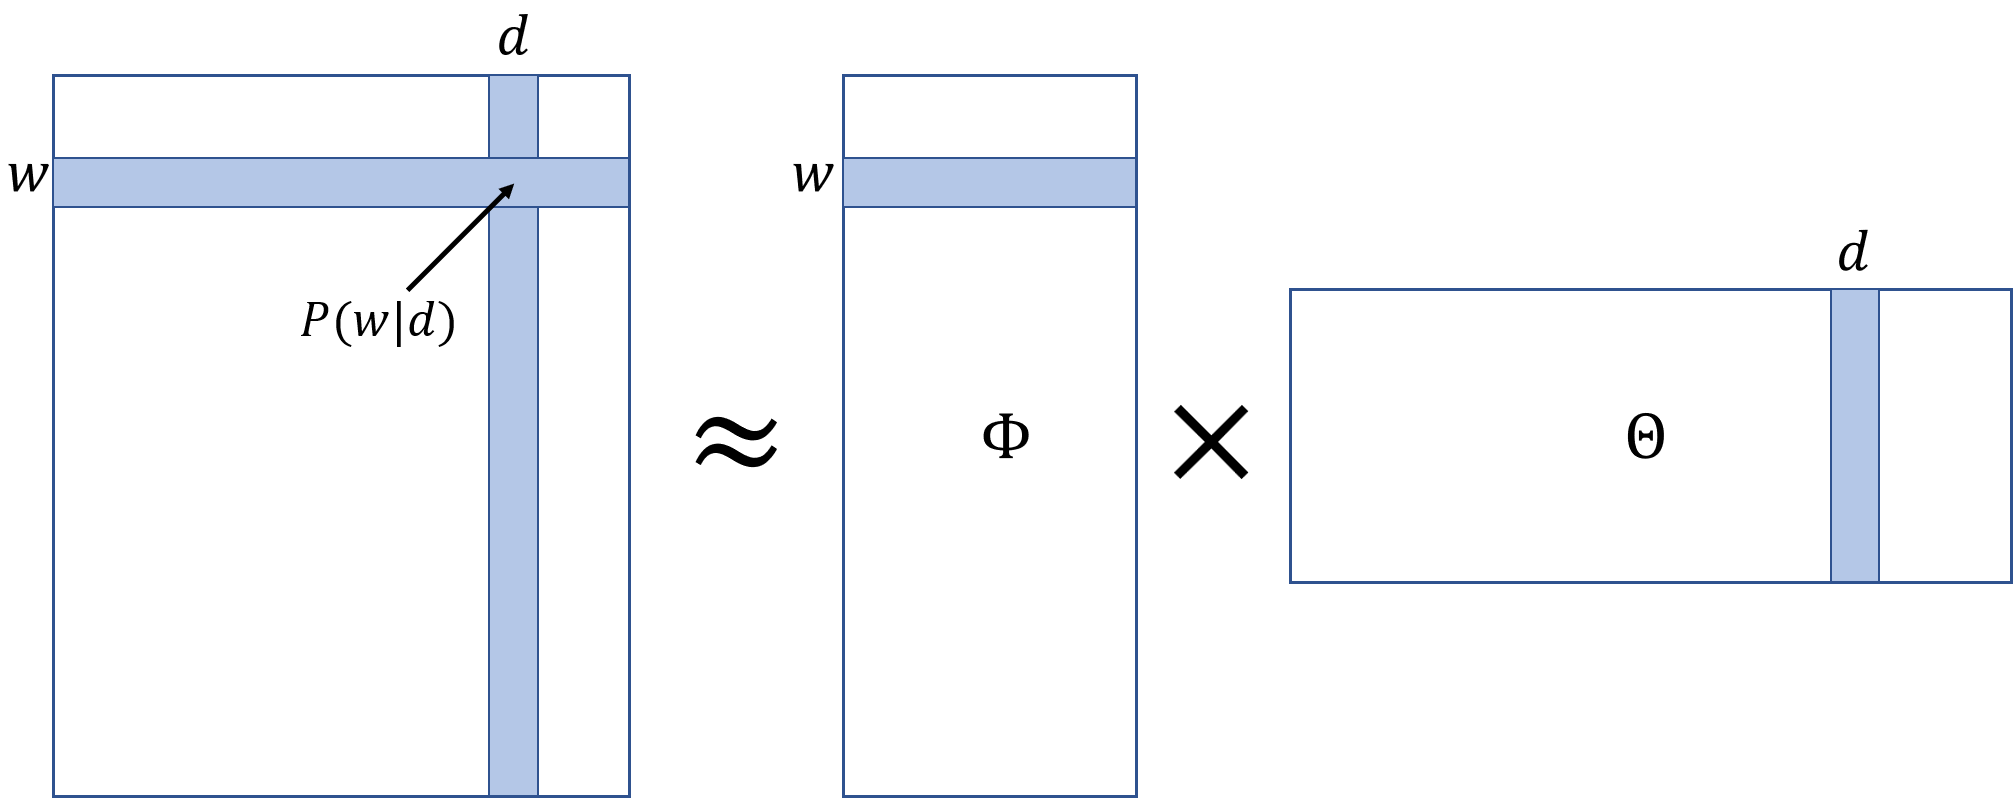
\includegraphics[scale=0.5]{svd.png}
    \caption{Стохастическое разложение матриц}
    \label{fig:svd}
\end{figure}
\subsection{Предварительная обработка текстов}
\subsubsection{Общие сведения}

\par
Часто решение задачи, каким-либо образом связанной с моделированием естественного языка, требует предварительной обработки текста, содержащей в себе:
\begin{itemize}
    \item приведение текста к единому регистру (обычно, нижнему);
    \item токенизацию -- разбиение текстов на более мелкие единицы (токены), которые могут быть различными по размеру, в зависимости от задачи;
    \item морфологическую разметку: с целью различать омонимы, несущие отличные семантические роли;
    \item удаление стоп-слов (слов, носящих излишне частотный или разреженный характер);
    \item лемматизацию (приведение слова к лемме -- нормальной <<словарной>> форме) или стемминг (сокращение слова до его основы);
    \item векторизацию слова: представление токенов в качестве численных векторов для последующей обработки.
\end{itemize}

\bigskip\par
Так как выбранный язык исследования английский, то морфологическая разметка особого результативного прироста не даст и ее можно опустить. После приведения текста к единому регистру и токенизации необходимо составить словарь слов текстов. Для оптимального построения словаря выполняется редуцирование слов (лемматизация) и удаление излишне частых и разреженных слов. Рассмотрим эти процессы подробнее.  
\subsubsection{Лемматизация и удаление стоп-слов}
\par
Минимальную информацию о текстовых данных можно получить с помощью понятий частоты. Закон Ципфа гласит, что наиболее часто употребимых слов лишь небольшое количество, тогда как подавляющее большинство слов используются существенно реже: частота любого слова в корпусе текстов обратна пропорциональна его рангу в таблице частот слов этого текста. Рассмотрим один из датасетов, на которых будет происходить последующее обучение моделей: отзывы на фильмы с платформы IMDB. Построим закон Ципфа в логарифмических координатах рис. \ref{fig:zipf}:
\[\ln r + \dfrac{1}{\alpha}\ln \omega_r = f(r),\]
где $r$ -- ранг слова в таблице частот, $\alpha \approx 1$ -- константа, $\omega_r$ -- абсолютная частота слова.
\begin{figure}[H]
    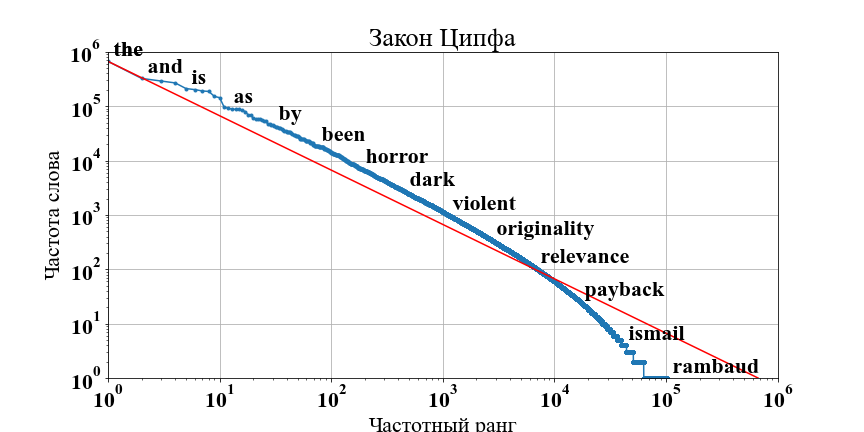
\includegraphics[scale=0.5]{zipf.png}
    \caption{Закон Ципфа на датасете IMDB}
    \label{fig:zipf}
\end{figure}

\bigskip\par
Явно заметен тренд к линейности, однако даже есть явное отклонение в районе слов с высоким ранжированием. Рассмотрим на распределения частот для позитивных и отрицательных комментариев (рис. \ref{fig:distribution_tokens_before_lemmatization}):
\begin{figure}[H]
    \centering
    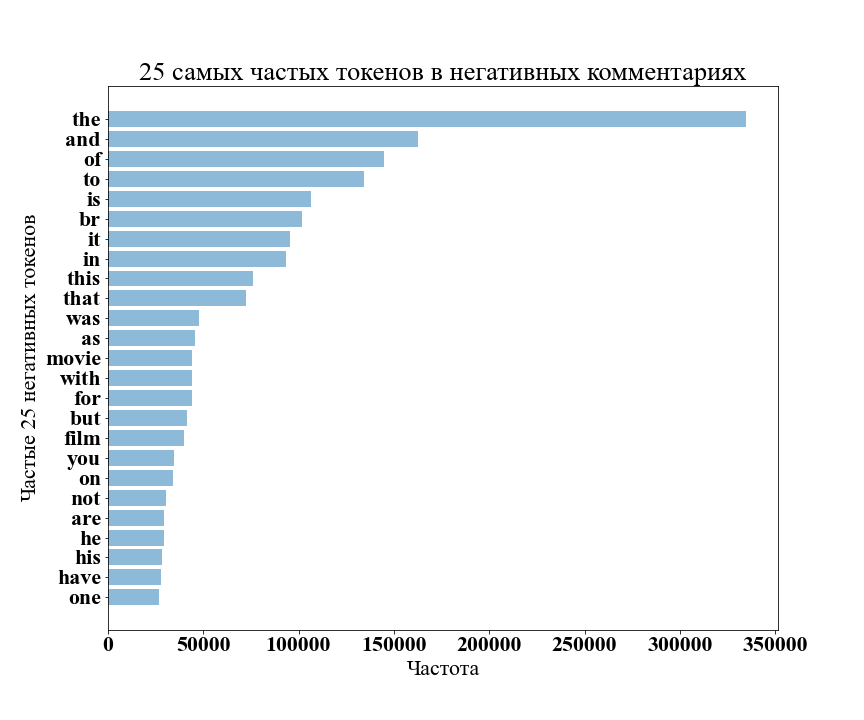
\includegraphics[scale=0.5]{negative.png}
    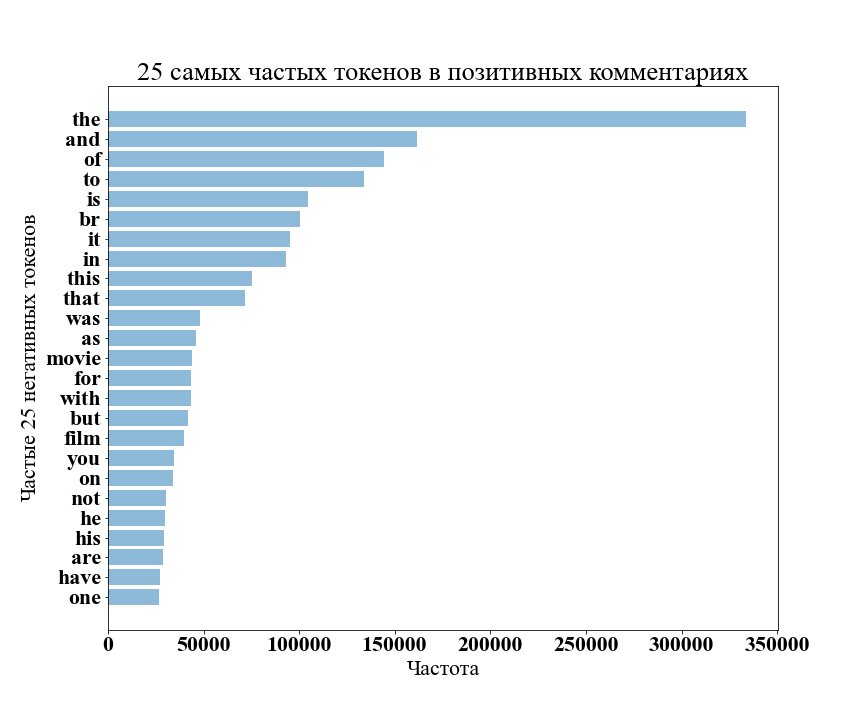
\includegraphics[scale=0.5]{positive.png}
    \caption{Самые частые слова в позитивных и негативных комментариях}
    \label{fig:distribution_tokens_before_lemmatization}
\end{figure}

\bigskip\par
Слова настолько часто встречающиеся усложняют процесс поиска закономерностей в текстовых данных. Похожее влияние оказывают и излишне редко встречающиеся слова: зачастую это либо профессионализмы или диалектизмы, либо слова с ошибками. Поэтому, помимо оптимальности построения словаря, в рамках задачи решение о применении этих методов предобработки текстов приведет к упрощению поиска заномерностей в итак сложно структурированных данных. Рассмотрим частотные характеристи после лемматизации и удаления стоп-слов (рис. \ref{fig:distribution_tokens_after_lemmatization})
\begin{figure}[H]
    \centering
    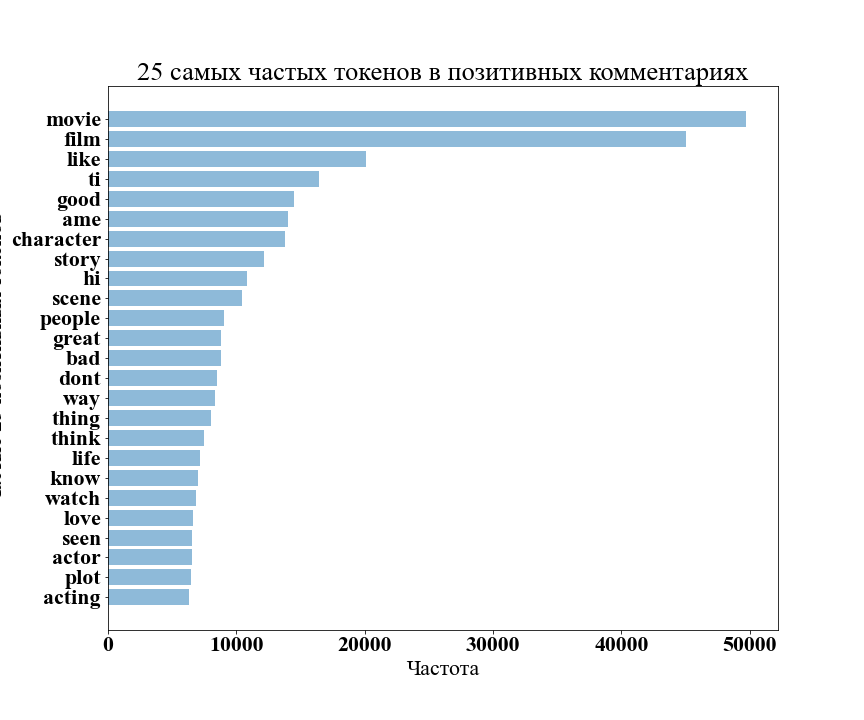
\includegraphics[scale=0.5]{positive_ac.png}
    \caption{Самые частые слова в позитивных комментариях после лемматизации и удаления стоп-слов}
    \label{fig:distribution_tokens_after_lemmatization}
\end{figure}

\bigskip\par
Позитивное влияние в виде упрощения структуры данных очевидно. Теперь необходимо представить предобработанные комментарии в векторном виде, чтобы в дальнейшем подавать их в модели глубокого обучения.

\subsubsection{Векторизация слов}
\paragraph{Bag of Words}
\par
Наиболее простым способом представления токенов в векторной форме является One Hot Encoding (OHE). Этот метод заключается в сопоставлении каждому токену вектора с размерностью, равной мощности словаря, и имеющего на всех позициях значения 0, кроме той, которая соответствует позиции самого токена в словаре, элемент с этим индексом равен 1 (рис. \ref{fig:ohe}).
\begin{figure}[H]
    \centering
    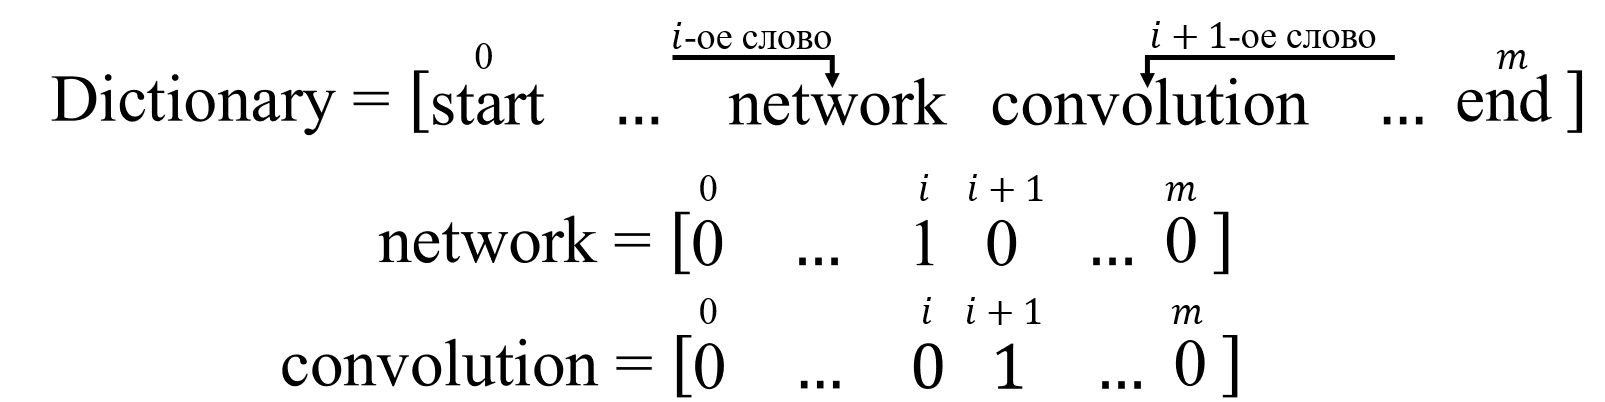
\includegraphics[scale=0.5]{ohe.png}
    \caption{One hot encoding (OHE) представление слов}
    \label{fig:ohe}
\end{figure}
\bigskip\par
Такой подход обладает достаточно закономерными недостатками:
\begin{itemize}
    \item вектора неинформативны: все векторы полученного пространства ортогональны друг другу, что не является полезным, причем большей информации о таком пространстве получить невозможно;
    \item большая размерность полученного пространства: с полученными векторами сложно оперировать функционально валидно из-за <<проклятия размерности>> \cite{curse};
    \item отсутствие возможности задать метрику в пространстве: слабая репрезентативность и отсутствие желаемых свойств пространству (арифметические операции над словами)
\end{itemize}
\bigskip\par
С целью получить количественную характеристику (частотную меру слов) применяется метод <<мешок слов>> \cite{harris54}. В работе метода выдвигается гипотеза о том, что порядок слов не несет в себе никакой информации. Получим векторы текстов путём сложения one-hot векторов токенов, в него непосредственно входящих рис. \ref{fig:bow}. 
\begin{figure}
    \centering
    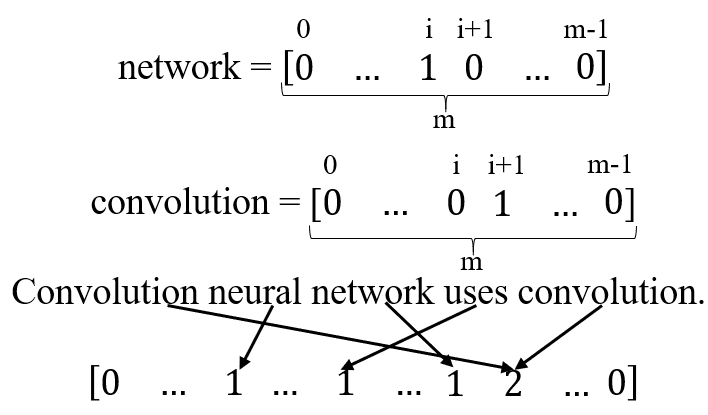
\includegraphics[scale=0.75]{bow.png}
    \caption{Bag of Words текстовое представление}
    \label{fig:bow}
\end{figure}
Такое представление так же содержит в себе немалое количество недостатков, среди которых: отсутствие информации о семантике и порядке слов. Однако эвристики и связанные с ними гипотезы оказываются полезными в дальнейшем. 
\paragraph{TF-IDF}
\par
Один из наиболее популярных способов векторизации в моделях машинного обучения. Все тексты представляются в виде матрицы $T = \left(t\right)_{d,w} = TF-IDF(w,d,D),$ где $d \in D$ -- текст, $w \in W$ -- слово в тексте. TF-IDF -- статистическая мера для оценки важности слова в контексте документа.
\[TF-IDF(w,d,D) = TF(w,d) \times IDF(w, D),\]
где $TF$ -- частота слова, которая оценивает слова в пределах документа (текста) по формуле:
\[TF(w,d) = \dfrac{n_i}{\sum\limits_{k}n_k},\]
где $n_i$ -- количество вхождений i-го слова в тексте. $\sum\limits_{k}n_k$ -- общее число слов в тексте. IDF вычисляется по формуле:
\[IDF(w,D) = \log \dfrac{|D|}{\{d_i \in D | w \in d_i\}},\]
где $|D|$ длина корпуса текстов, $\{d_i \in D | w \in d_i\}$ -- число текстов, в которых есть слово $w_i.$ 
\paragraph{Word2Vec}
\par
Word2Vec представляет собой полносвязную нейронную сеть с двумя различными архитектурами. В обоих случаях по тексту проходят скользящим окном размера $K$. Среди $K$ слов выделяют $K-1$ слов контекста и центральное слово. Первый тип Word2Vec Skip-gram (рис. \ref{fig:skipgram}) заключается в предсказывании контекста для слова:
\begin{figure}[H]
    \centering
    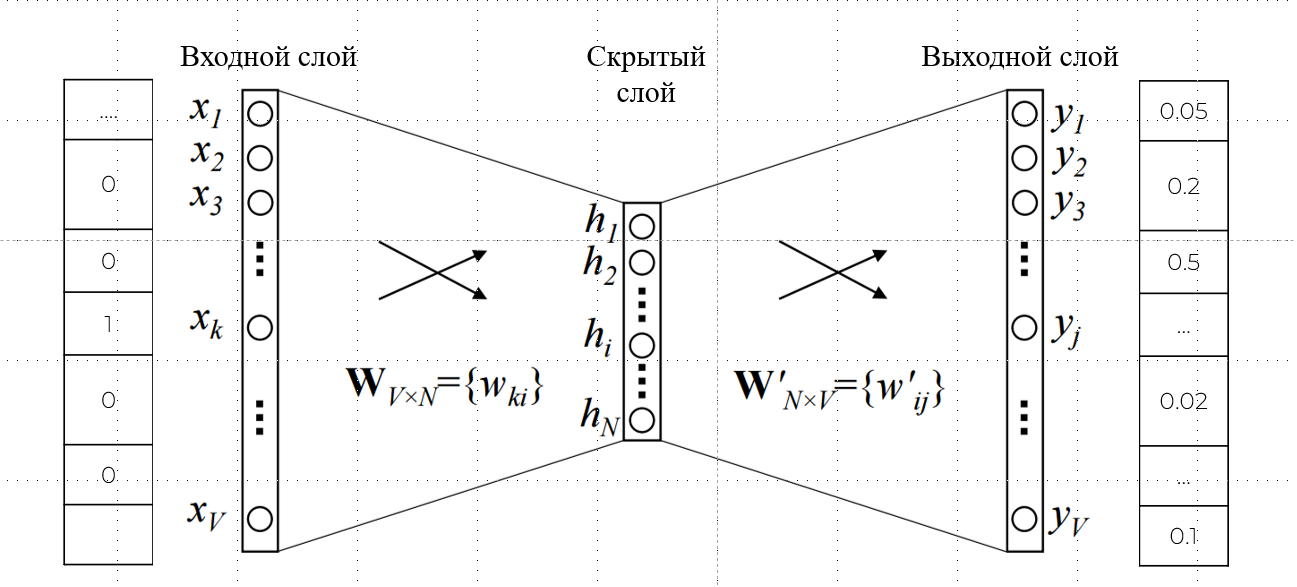
\includegraphics[scale=0.5]{skip-gram.png}
    \caption{Модель Word2Vec SkipGram \cite{mikolov2013distributed}}
    \label{fig:skipgram}
\end{figure}
\par
На выходе имеем $K-1$ мультиномиальных распределений вида:
\[P(c_k|i) = \dfrac{e^{u_{kc_k}}}{\sum\limits_{j'=1}^V e^{u_{j'}}}\]
Функция ошибки (loss Function):
\[L = -\ln P\left(c_1, \ldots, c_n| i\right) = -\sum\limits_{k=1}^{K}u_{kc_{k}} + n\ln\sum\limits_{j'=1}^V e^{u_j'}.\]
Для обучения будем максимизировать функцию правдоподобия:
\[L(\theta) = \prod_{d \in D}\left(\prod_{c \in C(i)} P(c|d; \theta)\right) = \prod_{\left(d,c\right) \in D} P(c|d; \theta),\]
где $C(i)$ -- множество возможных контекстных слов вокруг слова $i$ при обходе скользящим окном всего текста. Вектор вероятности определяется с помощью softmax вида:
\[P(c|d, \theta) = \dfrac{e^{\tilde w_c^Tw_d}}{\sum\limits{c'}e^{\tilde w_{c'}w_d}},\]
где $\tilde{w}_c$ -- вектор слова из контекста $c$, который отличается от $w_d$. Так как слова редко встречаются в контексте самих себя, то была придумана идеология использования двух разных векторов одного и того же слова (вместо одного), в первом случае слово будет выступать в качестве центрального в контексте, в другом контекстуальным. Этот метод описан в \cite{skipgram}. Выразим максимум логарифма функции правдоподобия:
\begin{gather*}
    \argmax\limits_{\theta} \prod_{(d,c)\in D} P(c|d;\theta) = \argmax\limits_{\theta} \sum\limits_{(d, c) \in D} \ln P(c|d; \theta ) =\\
    =  \argmax\limits_{\theta} \sum\limits_{(d,c)\in D} \sum\limits_{(d,c) \in D} \left(e^{\tilde{w}^T_cw_d} - \ln \sum\limits_{c'} e^{\tilde{w}_{c'}^Tw_d}\right)
\end{gather*}
\par
В статье \cite{cbow} приведен стохастический алгоритм оптимизации процедуры матричного умножения: $\sum\limits_{c} \tilde{w}_c^Tw_d$ negative sampling, заключающийся в выборе только нескольких элементов скалярного произведения весов  в качестве <<отрицательных примеров>>. Выведем измененную функцию правдоподобия:
\[\argmax\limits_{\theta} \prod_{(d,c) \in D} P((d,c) \in D; \theta) = \argmax\limits_{\theta} \]
Для простоты выразим вероятности через сигмоидную функцию активации (так как задача бинарной классификации, то softmax может быть заменен на sigmoid). Имеем:
\[P((d,c) \in D; \theta) = \dfrac{1}{1+e^{-\tilde{w}_c^Tw_d}}.\] Добавим набор отрицательных данных:
\[\argmax\limits_{\theta} \prod_{(d,c)\in D} P((d,c) \in D; \theta) \prod_{(d,c) \in D'}P((d',c') \not \in D; \theta)\]
Подставим с выражением для сигмоиды:
\begin{gather*}
    \argmax\limits_{\theta} \prod_{(d,c)\in D} P((d,c) \in D; \theta) \prod_{(d,c) \in D'} 1-P((d',c') \not \in D; \theta) = \\ 
    = \argmax\limits_{\theta} \left[\sum\limits_{(d,c)\in D} \ln P((d,c)\in D; \theta) + \sum\limits_{(d',c')\in D'} \ln(1-P((d',c')\not \in D; \theta))\right] = \\
    = \argmax\limits_{\theta} \sum\limits_{(d,c)\in D} \left[\ln \sigma(\tilde{w}_c^Tw_i) + \sum\limits_{(d,c')\in D'} \ln \sigma (-\tilde{w}_c^Tw_d)\right] 
\end{gather*}
Итоговая функция ошибки, для которой выполняется метод оптимизации:
\[L = \ln \sigma \left(\tilde{w}_c^Tw_i\right) \sum\limits_{(d,c')\in D'} \ln\sigma(-\tilde{w}_{c'}^Tw_i).\]
\bigskip\par
Модель CBOW предсказывает слово для контекста (рис. \ref{fig:cbow}):
\begin{figure}[H]
    \centering
    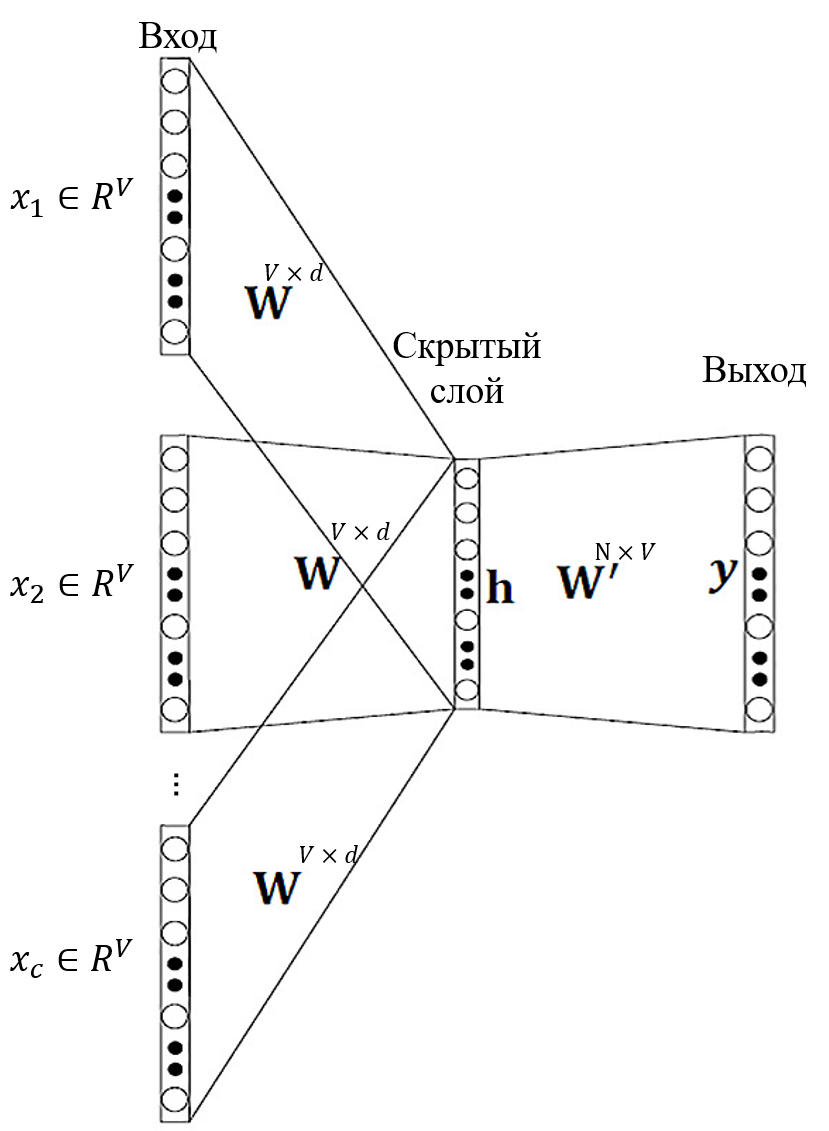
\includegraphics[scale=0.5]{cbow.png}
    \caption{Модель Word2Vec CBOW \cite{cbow}}
    \label{fig:cbow}
\end{figure}
Найдем апостериорное распределение модели с помощью softmax:
\[P(i|c_1,\ldots, c_n) = \dfrac{e^{u_j}}{\sum\limits_{j=1}^Ve^{u_j}}\]
Аппроксимируем с помощью функции потерь вида:
\[L = -\ln P(i|c_1,\ldots, c_n) = -u_j + \ln\sum\limits_{j=1}^V e^{u_j}\]
\paragraph{Embedding}
\par
С другой стороны возможно внедрение слоя Embedding непосредственно в архитектуру нейронной сети рис. \ref{fig:embedding}. Очевидным является вывод о лучшей статистике конечной модели с таким подходом, поскольку в результате обучения будет происходить подбор параметров слоя под конкретную задачу. Однако объектом исследований является значимость релевантной разницы метрики качества модели с использованием предобученных эмбеддингов Word2Vec и обучаемых слоев. Если эта разница будет незначительна, то валидным является использование предобученных моделей векторизации, поскольку они латентно содержат информацию о большем объеме слов в силу обучения на огромном корпусе текстов.
\begin{figure}[H]
    \centering
    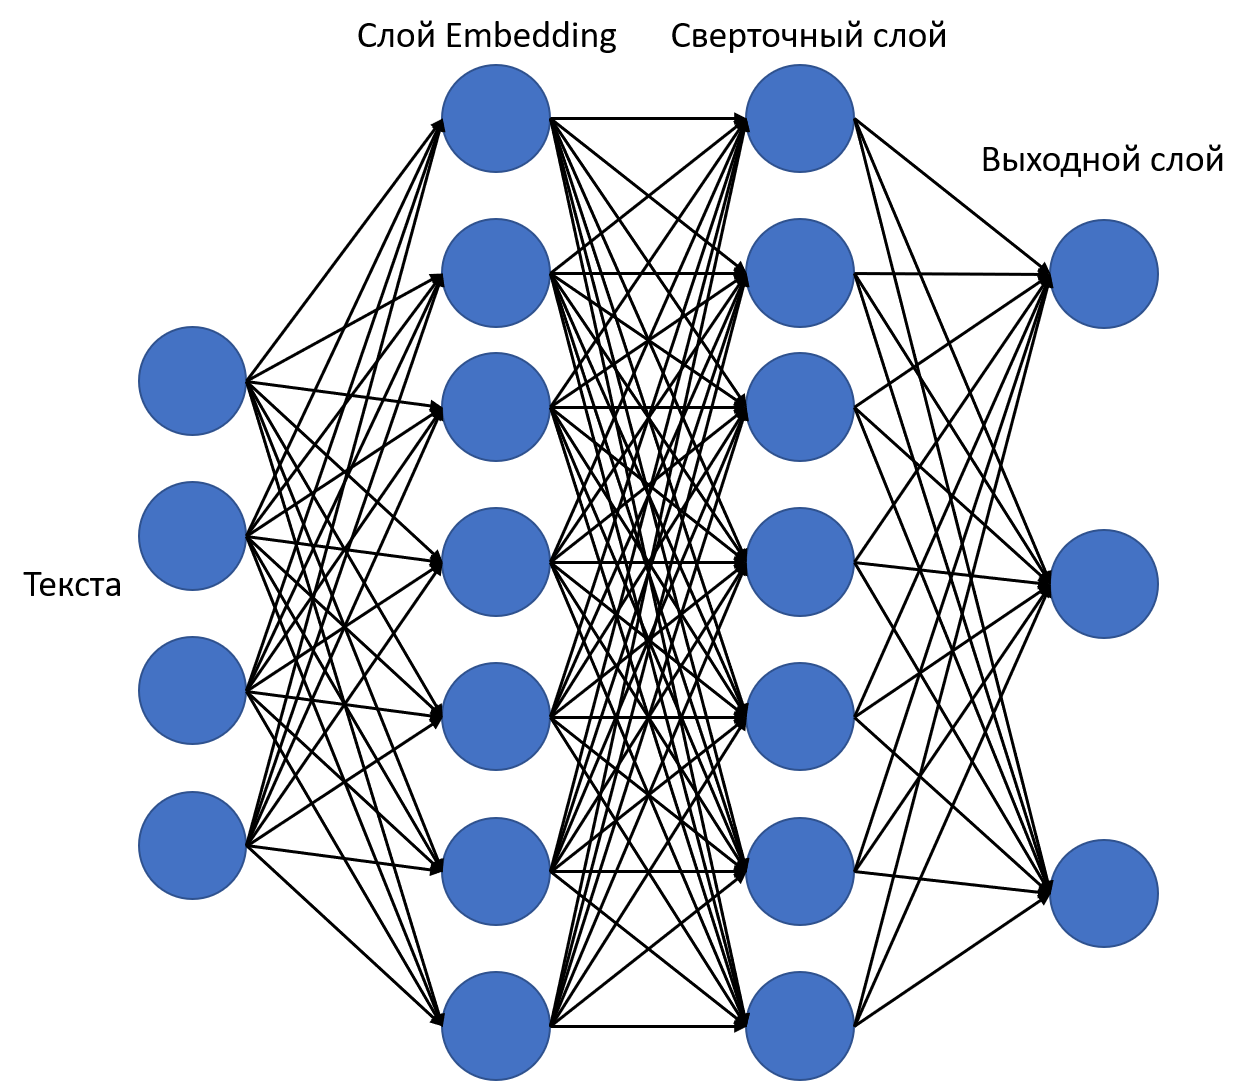
\includegraphics[scale=0.5]{embedding.png}
    \caption{Внедрение эмбеддингов непосредственно в архитектуру сети}
    \label{fig:embedding}
\end{figure}

\subsection{Нейронные сети}
\subsubsection{Сети прямого распространения}
\par
Целью сети прямого распространения является аппроксимация некой неизвестной функции $f$. Сеть состоит из однотипных элементов, называемых нейронами. Искусственный нейрон состоит из двух элементов: взвешенного сумматора и нелинейной функции активации над ним рис. \ref{fig:nn}.
\begin{figure}[H]
    \centering
    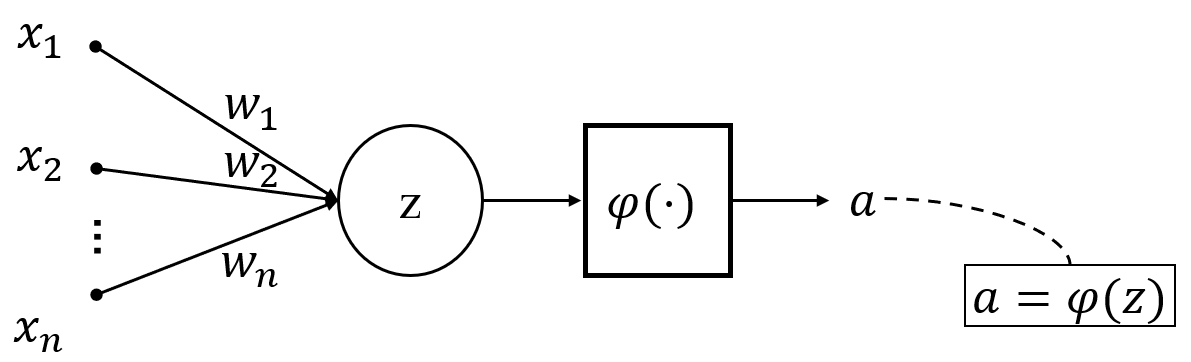
\includegraphics[scale=0.75]{nn.png}
    \caption{Модель искусственного нейрона}
    \label{fig:nn}
\end{figure}
Сумматор представляет собой выражение вида (скалярное произведение при введении $x_0 = 1$):
\[z = b + \sum\limits_{i=1}^n w_i x_i \stackrel{x_0=1}{=} w^Tx,\]
где $\vec x \in \mathbb{R}^n$ -- вектор признаков, $\vec w = \in \mathbb{R}^n$ -- вектор обучаемых параметров, $b \in \mathbb{R}$. Скопления нейронов называются слоями. Слой называется скрытым, если не определяет выход модели. Линейная композиция линейных преобразований способна представлять только линейные функции. Чтобы обобщить модель на представление нелинейных функций, вводится так называемая функция активации над результатом взвешенного сумматора. Вопрос сводится к выбору отображения. В книге \cite{Goodfellow} приведены три совета по выбору функции активации.
\subsubsection{Функции активации}
\begin{itemize}
    \item Бесконечномерная, используемая в ядерных методах (радиально-базисные) функция активации. Мощности такой функции хватит на аппроксимацию тренировочного набора, однако обобщаемость на тестовый датасет от этого страдает;
    \item Спроектировать функцию активацию $\varphi$ самостоятельно;
    \item Обучение функции активации $\varphi$. Модель представляется в несколько ином виде:
    \[y = f(x, \theta, w) = \varphi(x, \theta)^Tw.\]
    Преимуществом является выбор целого класса функций, однако придется подбирать новый гиперпараметр.
\end{itemize}
\bigskip\par 
Композиция линейных и нелинейных преобразований предоставляют универсальную аппроксимацию. Универсальная теорема аппроксимации \cite{hornik} утверждает, что сеть даже прямого распространения с линейным выходным слоем и нелинейным хотя одним слоем может аппроксимировать любую измеримую по Борелю функцию при условии, что в сети достаточно блоков. Однако эта теорема не говорит о том, насколько должна быть большой сеть. В работе \cite{barron} предпринята попытка дать верхние границы размера сети с одним уровнем -- экспоненциальное число блоков. Сети с одним слоем достаточно для универсального применения, однако этот слой может оказаться слишком большим: для решения этой проблемы под отдельные задачи берут конкретные архитектуры.

\bigskip\par 
Для классификации $n$ классов используется softmax -- функция вида:
\[\varphi(x) = \dfrac{e^{x_j}}{\sum\limits_{j=1}^Ve^{x_j}}.\]
\par
Для бинарной классификации может быть использована сигмоидная функция активации:
\[\varphi(x) = \dfrac{1}{1+e^{-x}}\]
\subsubsection{Обучение}
\par
Для обучения нейронной сети прямого распространения необходимо задать функцию ошибок между выходом сети $\tilde y$ и правильным результатом $y$. Алгоритм обратного распространения ошибки \cite{backpropagation} позволяет передавать информацию о функции ошибки обратно по сети для вычисления градиентов. Опишем граф вычисления сети прямого распространения. Пример -- граф для логистической регрессии рис. \ref{fig:logreg}:
\begin{figure}[H]
    \centering  
    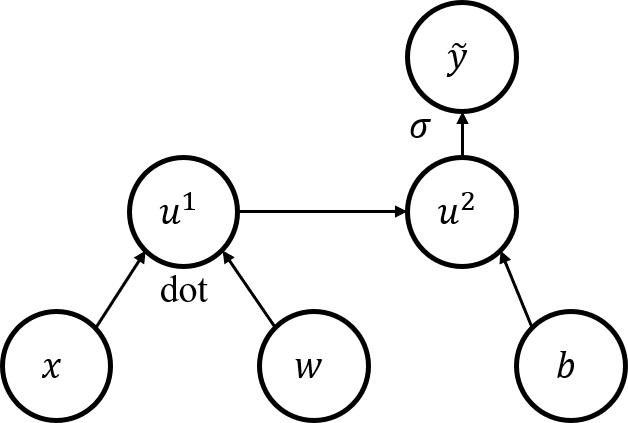
\includegraphics[scale=0.75]{log_reg.png}
    \caption{Граф вычислений для логистической регрессии}
    \label{fig:logreg}  
\end{figure}
Опишем алгоритм прохода по сети прямого распространения и вычисления функции ошибки (в общем случае с регуляризатором $\Omega(\theta)$):
\begin{algorithm}[H]
    \caption{Прямое распространение с регуляризатором $\Omega(\theta)$}\label{alg:cap}
    \begin{algorithmic}
        \State $W^{(i)}, \ i\in \left\{1, \ldots, l\right\}$
        \State $b^{(i)}, i \in \left\{1, \ldots, l\right\}$
        \State $x \gets \mathrm{input}$
        \State $y \gets \mathrm{label}$
        $s^{(0)} = x$
        \For{$k = 1, \ldots, l$}
            \State $a^{(k)} = b^{(k)} + W^{(k)}s^{(k-1)}$
            \State $s^{k} = f(a^{(k)})$
        \EndFor
        \State $\tilde y = s^{i}$
        \State $J = E(\tilde y, y) + \lambda\Omega(\theta)$
    \end{algorithmic}
\end{algorithm}
После вычисления прямого распостранения:
\begin{algorithm}[H]
    \caption{Обратное распространение ошибки}
    \label{alg:backprop}
    \begin{algorithmic}
        \State $g \gets \nabla_{\tilde y}J = \nabla_{\tilde y} E(\tilde y, y)$
        \For{$k = l, \ldots, 1$}
            \State $g\gets \nabla_{a^{(k)}}J = g \odot f'(a^{(k)})$
            \State $\text{Вычислим градиенты для смещений и весов (с регуляризацией)}$
            \State $\nabla_{b^{(k)}}J = g + \lambda\nabla_{b^{(k)}}\Omega(\theta)$
            \State $\nabla_{W^{(k)}}J = g s^{(k-1)} + \lambda\nabla_{W^{(k)}}\Omega(\theta)$

            \State $g \gets \nabla_{s^{(k-1)}}J = W^{(k)} g$
        \EndFor
    \end{algorithmic}
\end{algorithm}
Получив градиенты, можно интерпретировать эту информацию как указания о том, как следует изменить выходы слоев, чтобы уменьшить функцию ошибку. 
\subsection{Сверточные нейронные сети (CNN)}
Созданные для задач компьютерного зрения сверточные нейронные сети
\cite{LeCun:1, LeCun:2, LeCun:3} были
достаточно продуктивно применены и в других сферах глубокого обучения,
в том числе и NLP (natural language processing, 
обработка естественного языка).
Использование их достигло максимума в ответ на
ограниченность применения полносвязных сетей для обработки данных с сеточной топологией \cite{Goodfellow}.
\subsubsection{Операция свертки}
\textit{Определение:} Пусть $u, v: \ \mathbb{R}^{n} \to \mathbb{R}$ -- две функции, интегрируемые относительно меры Лебега
    на пространстве $\mathbb{R}^{n}$. Тогда функция  $u * v: \ \mathbb{R}^n \to \mathbb{R}$ называется сверткой
    и определяется соотношением:
    \[(u * v) (x) := \int\limits_{\mathbb{R}^{n}} u(y)v(x-y)dy,\]
    где $y$ иногда называют давностью, $u$ -- входом, $v$ -- ядром свертки (kernel). Результат
свертки именуется картой признаков (feature map).
В задаче классификации текстов в силу плоского векторного представления слов будем рассматривать
одномерную свертку. Для $n = 1$ формула примет вид:
\[(u * v) (x) := \int\limits_{-\infty}^{\infty} u(y) v(x-y)dy\]
Кроме того, задача представляет собой конечный, дискретный случай, значит, окончательный вид формулы:
\[(u * v) (x) := \sum\limits_{y = 0}^{K} u (y) v(x-y),\]
%! проверить K
где K -- размер ядра.

Для иллюстрации операции свертки рассмотрим функции $u, v$ как сигналы рис. \ref{fig:cnn1}.
\begin{figure}[ht]
    \centering
    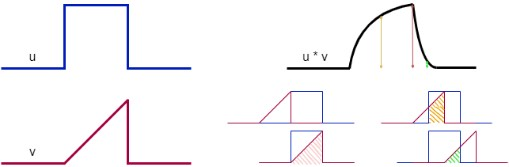
\includegraphics[scale=2]{convolution.jpg}
    \caption{Операция свертки между двумя сигналами $u,v$}
    \label{fig:cnn1}
%! добавить названия рисунков
\end{figure}
Сдвигая ядро $v$ относительно входного сигнала $u$ и, посчитав скалярное произведение векторов, 
получим сходство фрагмента сигнала с ядром, что и является результатом свертки.
\subsubsection{CNN для работы с изображениями}
Для изображений характерно матричное представление, 
каждому элементу которого соответствует значение пикселя. 
На рис. \ref{fig:cnn2}
приведен случай с изображением размерности $5 \times 5 \times 1$.  
\begin{figure}[ht]
    \centering
    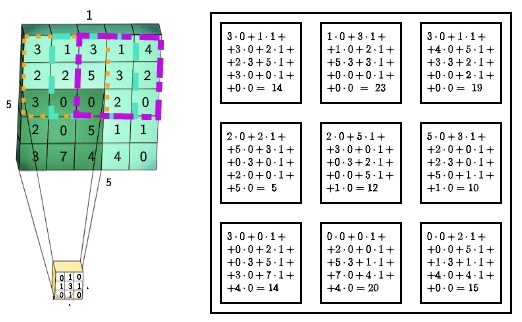
\includegraphics[scale=1]{convolution_images.png}
    \caption{Пример операции свертки для изображения $5\times 5\times 1$ с ядром свертки $3\times 3\times 1$}
    \label{fig:cnn2}
\end{figure}
Ядро свертки (размерности $3 \times 3 \times 1$) прикладывается к каждому фрагменту изображения с задаваемым шагом (stride). 
На Рис. \ref{fig:cnn2} приведен пример со значением шага, равным единице.
Видно, что каждый нейрон связан лишь с частью пикселей, если речь идет о первом сверточном слое или нейронов, 
для последующих слоев (это свойство называют разреженной связностью). Необходимым становится обучение лишь значений ядер свертки, 
что значительно меньше, чем в случае традиционных нейронных сетей (полносвязных).
\subsubsection{Одномерные CNN для работы с текстами}
Как уже было сказано ранее, слова (после векторизации) представляют собой плоские вектора. Поэтому для задач обработки естественного 
языка применяются одномерные сверточные нейронные сети. Токены (в рассматриваемом случае, слова), представленные в векторной форме,
конкатенируются в матрицу текста.
Затем выбирается $k$ строк матрицы, которые вытягиваются в плоский вектор. К нему прикладывается (берется скалярное произведение) 
одномерное ядро размерности $k \cdot s$, где $s$ -- размерность вектора токена. Этот процесс иллюстрирован на рис. \ref{fig:cnn31} 
и рис. \ref{fig:cnn32}. 
\begin{figure}[H]
    \centering
    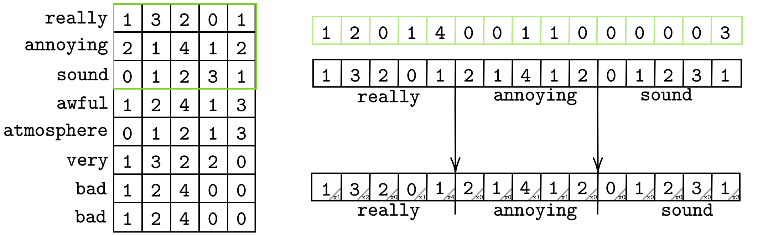
\includegraphics[scale=1.5]{convolution_text_1.png}
    \caption{Применение свертки для извлечения признаков из текста}
    \label{fig:cnn31}
\end{figure}
Двигаясь таким образом по матрице текста, можно получить столбец значений – результатов операции одномерной свертки. 
Для получения большего количества столбцов, которые, в свою очередь, образуют матрицу признаков, используется несколько ядер.
\begin{figure}[H]
    \centering
    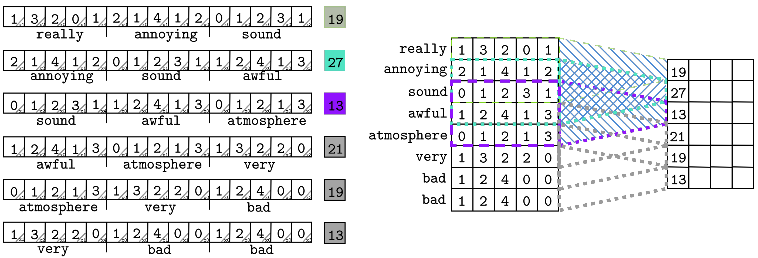
\includegraphics[scale=1.5]{convolution_text_2.png}
    \caption{Применение свертки для извлечения признаков из текста}
    \label{fig:cnn32}
\end{figure}
После применения операции свертки как для изображений, так и для других структур, в том числе и текстов,
 возможно применение слоя субдискритизации (Pooling, подвыборки). Пулинг работает подобно сверточному слою, 
 однако вместо скалярного произведения применяет другие функции на фрагменты, 
 например, возвращает максимальный или средний выходы в прямоугольной окрестности
  (max-пулинг \cite{Zhou:1} и average-пулинг соответственно). \\Max-Pooling:
  \[f_{MP} = \max\limits_{i} x_{i}.\] 
  Average-Pooling:
  \[f_{AP} = \frac{1}{n} \sum\limits_{i=1}^{n}x_{i}.\]
  \bigskip\par
  Логика употребления слоя пулинга заключается в том, что выявленные сверточным слоем закономерности избыточны 
  в своей подробности, значит, возможно уплотнение до менее подробного результата. Однако, если в задаче необходимо 
  сохранять точную пространственную информацию, применение пулинга по всем признакам существенно увеличивает ошибку модели,
  что исследовано экспериментально \cite{Szegedy2014}. Сверточный слой и слой пулинга, следующий за ним, образуют сверточный блок.
   Чем больше количество сверточных блоков, тем более абстрактной или высокоуровневой становится карта признаков.
   \bigskip\par
Заключим, что сверточная нейронная сеть достаточно успешно решает задачу извлечения признаков из данных.
 Экстраполируем этот вывод на одномерную плоскость для работы с текстами: сверточные нейронные сети, извлекая закономерности в текстовых данных, 
 способны различать контекст. Причем ширину контекста можно приблизительно идеализировать шириной рецептивного поля (или пятна восприятия). 
 На рис. \ref{fig:cnn4} ширина рецептивного поля на первом слое равна трем, а ширина рецептивного поля на втором слое равна четырем, 
 таким образом происходит расширение контекста. Однако всё же речь идет о, с точки зрения языка, маленьких паттернах, словосочетаниях 
 и коротких фразах. Для масштабного и более полного моделирования языка необходимо делать очень глубокие сети, что неминуемо приводит к
 увеличению числа обучаемых параметров.
\begin{figure}[H]
    \centering
    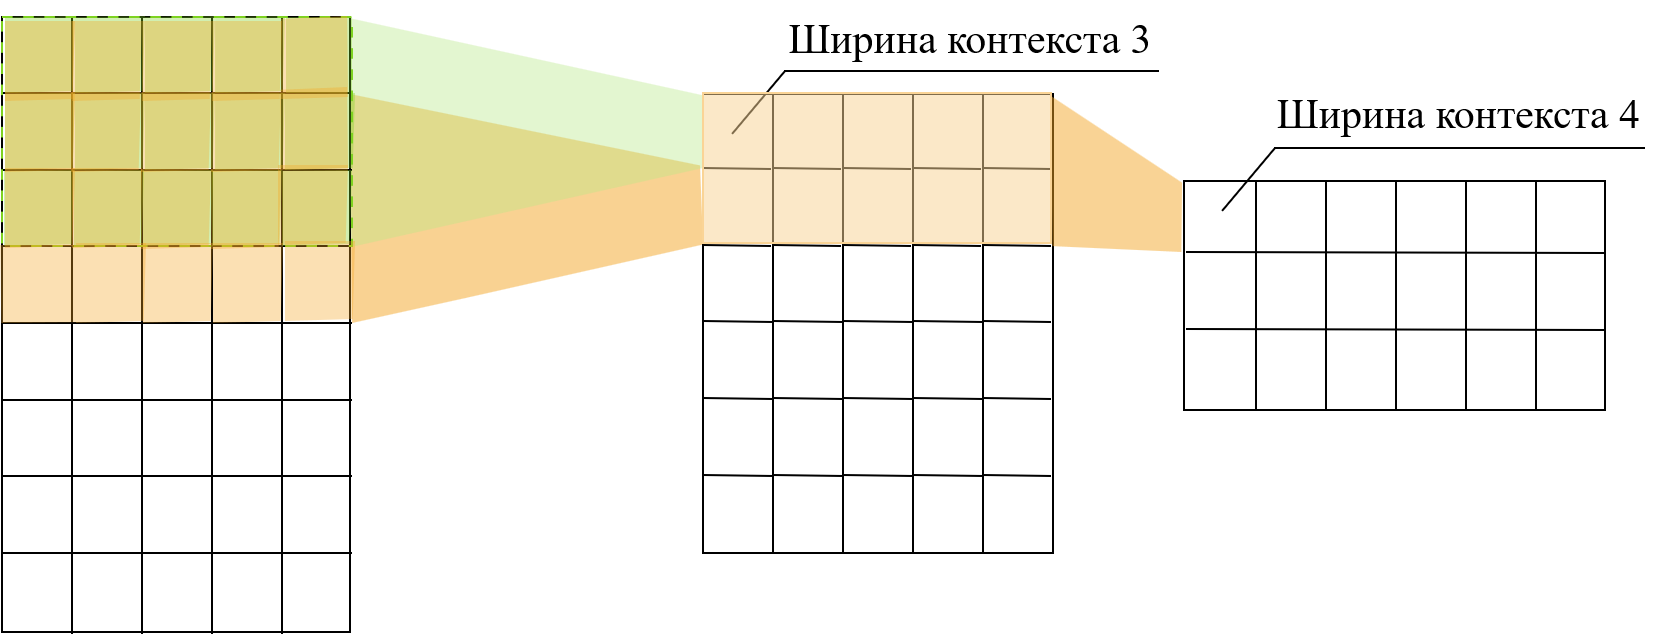
\includegraphics[scale=0.5]{context_width}
    \caption{Ширина рецептивных полей}
    \label{fig:cnn4}
\end{figure}
Существует другой способ увеличения ширины контекста, который, так же как и пулинг, является спорным в употреблении в некоторых условиях задач:
прореживание (dilation) \cite{Srivastava:1}. Заключается он в применении свертки к фрагменту, из которого удалена часть элементов. Например,
возьмем $k$ строк не подряд, а через одну, но значит это то, что мы пропускаем каждое второе слово, что не может однозначно сказаться на решаемой проблеме.
\bigskip\par
Для решения задачи классификации после череды сверточных блоков (сверточный слой + слой пулинг) конечную карту признаков любой размерности, в зависимости от предыдущих слоев,
необходимо растянуть в вектор и подать в полносвязный слой с функцией активации SoftMax (для классификации $n$-классов, $n\in\mathbb{N}$) или Sigmoid (для бинарной классификации),
чтобы получить вероятности классов. 
\bigskip\par
Формула размерности карты признаков, учитывая всевозможные преобразования, после применения сверточного слоя или пулинга:
\[L_{\text{вых}} = \frac{L_{\text{вх}} + 2 \cdot \mathrm{padding} - \mathrm{dilation} \cdot (\mathrm{kernel\textunderscore size} -1) -1}{\mathrm{stride}} + 1,\]
где $\mathrm{padding}$(замощение) -- параметр, используемый в случае, когда есть необходимость в сохранении размерности при выполнении свертки или пулинга: недостающие элементы
для этого заполняются нулями. 
\subsubsection{Преимущества, недостатки и способы борьбы с ними}
% ? редактировать!!!
Сверточные нейронные сети хорошо находят закономерности в пространственных данных. Для текста эти зависимости именуются контекстом, идеализацией которого является ширина рецептивных полей сети. 
Так как вычислительные ресурсы ограничены, то построение очень глубоких сетей такой архитектуры затруднительно.
Ширина рецептивных полей сверточных нейронных сетей позволяет определять частичный контект текстовой информации:
прореживание и пулинг дают возможность увеличить контекст, однако их использование требует достаточной осторожности и может привести к росту ошибки. 
Это не мешает отлично справляться с задачей классификации текстов одномерным сверточным сетям, что доказывают результаты. Но всё становится значительно хуже при попытках моделирования языка. К тому же,
сверточные нейронные сети, как и традиционные, требуют входные данные фиксированной длины, что накладывает ограничение на плоское пространство текстов. В среднем, такие ограничения не оказывают критичного влияния, 
но объемные текста могут нести важные для классификации детали в той своей части, которую не покрывает выбранный масштаб анализа. 
\subsection{Рекуррентные нейронные сети (RNN)}
В случае сверточных нейронных сетей, текст позиционировался как пространственная структура. 
В случае рекуррентных нейронных сетей \cite{Schmidhuber2015, Schmidhuber:1996} следует рассматривать его как последовательность,
информация об элементе которой находится в зависимости от предшествующих ему элементов, 
другими словами, текст имеет направленное повествование. 
Подобная структура присуща не только текстам, но также и аудиосигналам или временным рядам.  
\subsubsection{Традиционные RNN}
Основная идея рекуррентных нейронных сетей зиждется на введении скрытых состояний 
и определении новых состояний через предыдущие. Таким образом, происходит латентное запоминание информации.
 То есть, в отличие от других нейронных сетей (сверточных, полносвязных), рекуррентная определяет своё состояние 
 не только за счет входных данных, но и за счет предыдущих состояний.
 \begin{figure}[ht]
     \centering
     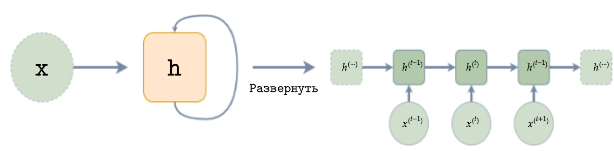
\includegraphics[scale=2]{rnn1}
     \label{rnn1}
     \caption{Развернутая рекуррентная нейронная сеть без выходов}
 \end{figure}
 
 На каждом шаге рекуррентной сети:
 \begin{enumerate}
     \item Прочитать очередной элемент последовательности $x^{t}$,
      применить к нему линейное преобразование:
      \[z^{t} = W_{\text{input}} \cdot x^t;\]
     \item Вычислить новое значение состояния, исходя из старого:
      \[h^{t} = \mathrm{act} \left(W_{\text{hidden}} \cdot h^{t-1} + z^{t}\right);\]
     \item Выйти из рекуррентного шага:
      \[y^{t} = W_{\text{output}} \cdot h^{t}.\]
 \end{enumerate}

 \bigskip\par
 Обучаемыми параметрами являются веса $W_{\text{input}}, W_{\text{hidden}}, W_{\text{output}}$, участвующие в линейных преобразованиях.
Нулевое состояние сети может задаваться различными способами: исходя из экспериментальных показателей, лучше всего использовать малодисперсный шум \cite{Goodfellow}.

\bigskip\par
Основными проблемами рекуррентных нейронных сетей во время обучения являются сходимости: возникают взрыв и затухание градиента. Рассмотрим эти ситуации подробнее.
\subsubsection{Затухание и взрыв градиента}
Рассмотрим прямой проход (forward pass) по классической рекуррентной нейронной сети (Vanilla RNN) на рис. \ref{fig:rnn3} 
\begin{figure}[ht]
    \centering
    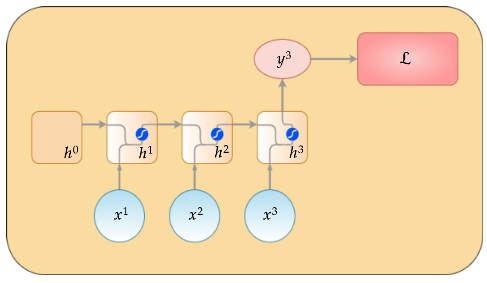
\includegraphics[scale=1.5]{rnn3.png}
    \caption{Vanilla RNN}
    \label{fig:rnn3}
\end{figure}

Введем обозначения. Входная последовательность $x^{t} \in \mathbb{R}$, скрытое состояние $h^{t} = f(w\cdot h^{t-1} + x^{t}),$ где $f$ -- нелинейная, дифференцируемая функция активации, $w \in \mathbb{R}$ -- параметр функции перехода, $y^{t} = g(h^{t})$ -- выход, функция потерь (функция ошибки, функционал качества) $\mathcal{L}(y^{t})$:
\begin{enumerate}
    \item $h^{0} \in \mathbb{R}$;
    \item $h^{1} = f(w\cdot h^{0} + x^1)$;
    \item $h^{2} = f(w\cdot h^{1} + x^{2}) = f\left(w \cdot f \left(w \cdot h^{1} + x^{2}\right) + x^{3}\right) = \\\hspace{0.5cm}=f\left(w \cdot f\left(w \cdot f\left(w \cdot h^{0} + x^{1}\right) + x^{2}\right) + x^{3}\right).$
\end{enumerate}
Выполним обратный проход (back propogation through time \cite{Zipser:1}):
\begin{gather*}
\mathcal{L} (y^{3}) = \mathcal{L} \left(g\left(h^{3}\right)\right) = \mathcal{L}\left(g\left(f\left(w\cdot h^{2} + x^{3}\right)\right)\right) = \\ = \mathcal{L}\left(g\left(f\left(w\cdot f\left(w\cdot h^{1} + x^{2}\right) + x^{3}\right)\right)\right)    
\end{gather*}
Применяя градиентный спуск, нам понадобится производная по параметрам:
\[\frac{\partial \mathcal{L}\left(y^{3}\right)}{\partial w} = \frac{\partial \mathcal{L}\left(y^{3}\right)}{\partial g}\cdot \frac{\partial g}{\partial w} = \frac{\partial \mathcal{}{L}\left(y^{3}\right)}{\partial g} \cdot \frac{\partial g}{\partial f}\cdot \frac{\partial f\left(w\cdot h^{2} + x^{3}\right)}{\partial w}\]
\begin{gather*}
    \frac{\partial f\left(w\cdot h^{2} + x^{3}\right)}{\partial w} = f'\left(w\cdot h^{2}+ x^{3}\right)\cdot \left(w\cdot h^{2} + x^{3}\right)' = f_{3}'\cdot \left(w \cdot h^{2}\right)' = \\ = f_{3}'\left(w'\cdot h^{2} + w \cdot h^{2'}\right) - f_{3}'\cdot \left(h^{2} + w\cdot f\left(w \cdot h^{1} + x^{2}\right)'\right) = \\ = f_{3}'\cdot \left(h^{2}+ w\cdot f_{2}' \cdot \left(h^{1} + w\cdot f\left(w\cdot h^{0}+ x^{1}\right)'\right)\right) = \\ = \sum\limits_{i = 1}^{3} \left(h^{i-1} \cdot w^{3-i}\prod\limits_{j=i}^{3}f_{j}'\right)
\end{gather*}
Именно последнее умножение является причиной затухания или взрыва градиента. Одной из часто употребляемых функций активаций является гиперболический тангенс, производная которого лежит в диапазоне: $0 < \tanh' < 1$.
Умножение большого числа таких значений приведет к затуханию градиента (vanishing gradient) \cite{Zipser:1}. Борьбой с этим является ограничение количества скрытых состояний, что, по сути, ограничивает обрабатываемые последовательности. Основная идея рекуррентных нейронных сетей теряет смысл при подобном решении проблемы.

\bigskip\par
С другой стороны, если модуль произведения больше единицы, то произойдет взрыв градиента, приводящий к переполнению и падению точности. Борьба с такой проблемой является более очевидной -- ограничение на сам градиент (ввод фиксированной величины, превышение которой ограничивает превысивший ее градиент этой величиной). 

\bigskip\par
Затухающий градент так же связан с долгосрочными зависимостями \cite{Schmidhuber2001}. Любые флуктуации в краткосрочных зависимостях буду подавлять долгосрочные. В случае, если модель способна представить долгосрочные зависимости, градиент долгосрочного взаимодействия будет экспоненциально ниже краткосрочного \cite{Goodfellow}.

\bigskip\par
В связи с таким поведением градиента при обучении возникает явная проблема борьбы между мощностью и обучаемостью рекуррентных сетей. Ради ее решения были разработаны специализированные архитектуры рекуррентных нейронных сетей: LSTM \cite{Schmidhuber:1996} и GRU \cite{Sutskever:1}.
\subsubsection{Долгая краткосрочная память (LSTM)}
Сеть LSTM \cite{Schmidhuber:1996} использует концепцию вентильных нейронных сетей (gated Recurrent Neural Networks), основанную на идее контролированного выбора путей между состояниями. Путей, на которых не обнуляются и не устремляются в бесконечность производные. Веса связей скрытых состояний в такой структуре могут изменяться на каждом временном (или пространственном, зависит от структуры анализируемых данных) шаге. На рис. \ref{fig:lstm1} и \ref{fig:lstm2} представлены срез LSTM слоя и LSTM блок, соответственно.
\begin{figure}[H]
    \centering
    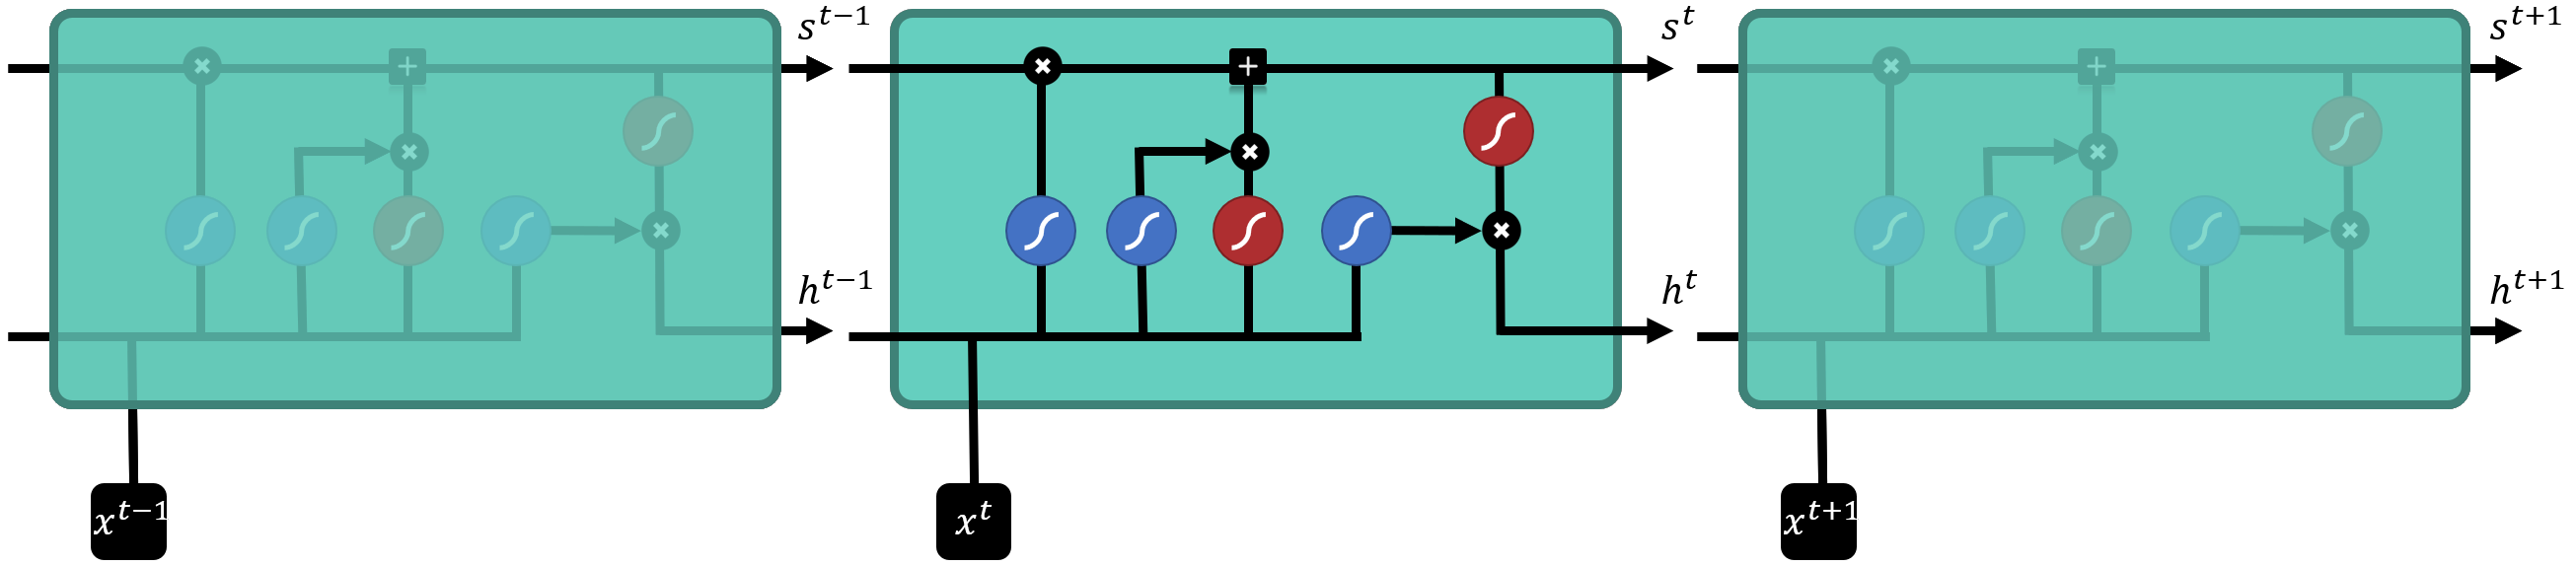
\includegraphics[scale=0.35]{lstm1.png}
    \caption{Срез развернутого LSTM слоя.}
    \label{fig:lstm1}
\end{figure}
Идея вентилей состоит в том, чтобы контролировать вектор значений за счет его умножения на вектор шлюза (вентиля), который управляет потоком ошибки. Целью является сохранение постоянного объема потока ошибки.\\
\begin{figure}[ht]
    \centering
    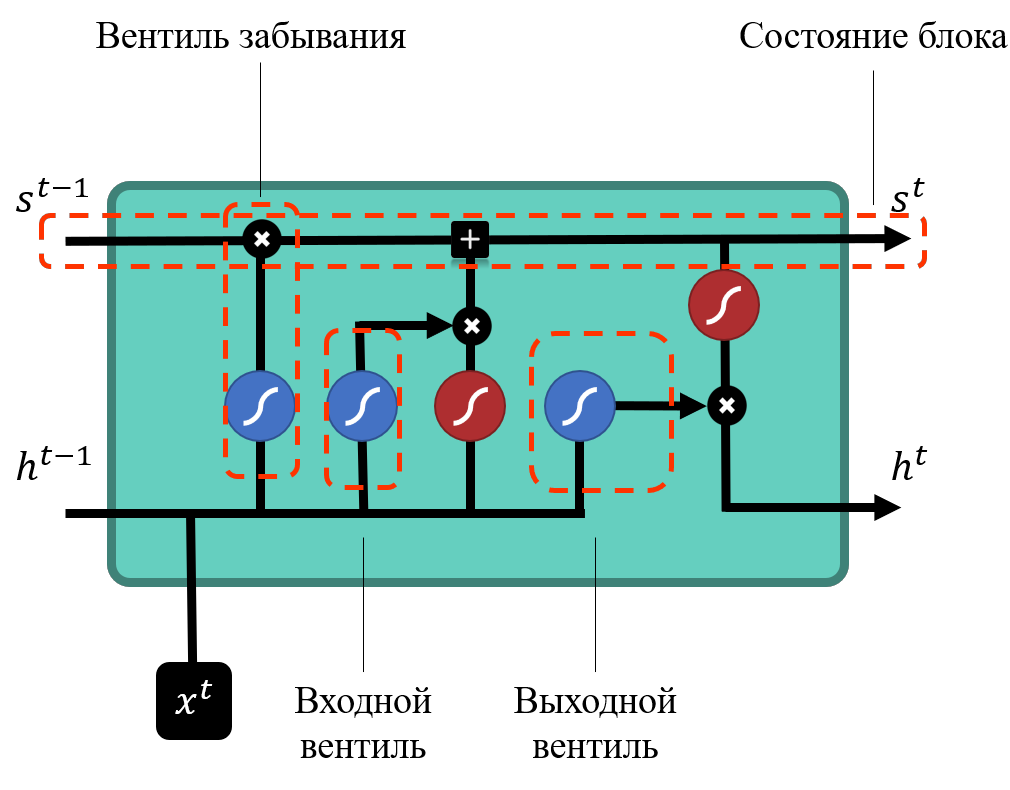
\includegraphics[scale=0.7]{lstm2.png}
    \caption{LSTM блок.}
    \label{fig:lstm2}
\end{figure}

\bigskip\par
Запишем формальный прямой ход LSTM блока в момент времени $t$:
\begin{itemize}
    \item Конкатенируем прошлое скрытое состояние $h^{t-1}$ и входной вектор $x^{t}$. Применяем линейное преобразование и нелинейную функцию активации:
    \begin{gather*}
        f_{t} = \sigma\left(W_{f}\cdot \left[h^{t-1}, x^{t}\right] + b_{f}\right);\\
        i_{t} = \sigma \left(W_{i}\left[h^{t-1}, x^{t}\right] + b_{i}\right);\\
        \tilde{s}^{t} = \mathrm{act}\left(W_{\tilde{s}}\cdot \left[h^{t-1}, x^{t}\right] + b_{\tilde{s}}\right);\\
        o_{t} = \sigma \left(W_{o} \cdot \left[h^{t-1}, x^{t}\right] + b_{o}\right);
    \end{gather*}
    $\mathrm{act}$ -- функция активации (например, $\tanh$);
    \item Получим сигнал как линейную комбинацию:
    \[s^{t} = f_{t} \cdot s^{t-1} + i_{t} \cdot \tilde{s}^{t};\]
    \item Выходим из рекуррентного шага:
    \[h^{t} = o_{t}\cdot \tanh (s^{t}).\]
\end{itemize}
$f_{t}$ -- вентиль забывания (forgetting gate), обучаемый за счет весов $W_{f}$ и сдвига $b_{f}$, определяющий насколько нужно забыть состояние с прошлого блока.\\
$i_{t}$ -- входной вентиль (input gate), обучаемый за счет весов $W_{i}$ и сдвига $b_{i}$, ответственный за чувствительность ко входу: определяет, насколько важно для запоминания полученное новое состояние $\tilde{s}^{t}$. Состояние $\tilde{s}^{t}$ в рекуррентных сетях без вентильной парадигмы было бы выходом блока.\\
$o_{t}$ -- выходной вентиль (output gate), применяемый для увеличения точности аппроксимации нейронной сети за счет нелинейности функции активации.

\bigskip\par
За счет того, что сигмоида принимает значения в диапазоне: $0 < \sigma < 1$, все значения вентилей находятся в этом же диапазоне, что позволяет управлять амплитудой значений состояний, не меняя знак и контролируя объем потока ошибки. \\
Внутренние работы с новыми и старыми состояниями позволяют классифицировать их важность, как следствие настроить запоминание и забывание того, что нужно для решения задачи и бесполезно, соответственно. LSTM достаточно успешно представляет долгосрочные зависимости, моделирует язык, позволяет решать широкий спектр задач, но не лишена проблем. За счет появления новых внутренних обучаемых весов и сдвигов увеличивается количество обучаемых параметров в 4 раза по сравнению с обычной рекуррентной нейронной сетью. Поэтому LSTM часто может переобучаться и показывать плохие результаты на новых данных.
\subsubsection{Управляемый рекуррентный блок (GRU)}
Уменьшить количество обучаемых параметров без сильной потери качества удалось сети GRU (gated recurrent unit, управляемый рекуррентный блок). Основная идея остается той же -- сохранение постоянства объема потока ошибки.
\begin{figure}[H]
    \centering
    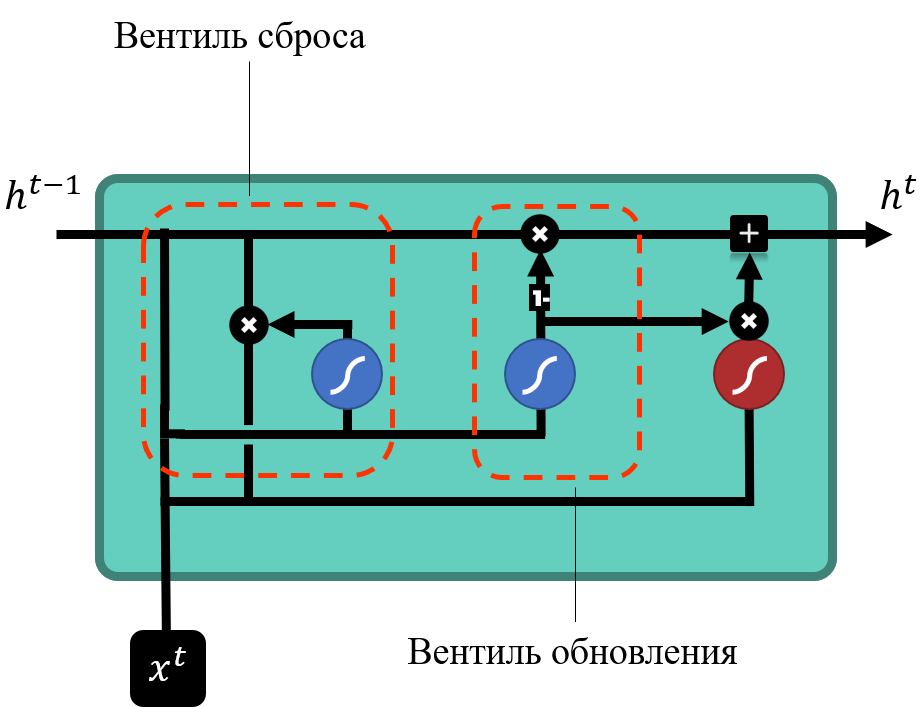
\includegraphics[scale=0.7]{gru1.png}
    \label{gru1}
    \caption{GRU блок}
\end{figure}

\bigskip\par
Запишем формальный прямой ход GRU блока в момент времени $t$:\\
\begin{itemize}
    % \setlength\itemsep{-0.5cm}
    \item Конкатенируем $h^{t-1}$ и $x^{t}$. Применяем линейное преобразование и нелинейную функцию активации:
    \begin{gather*}
        u_{t} = \sigma \left(W_{u} \cdot\left[x^{t}, h^{t-1}\right]\right);\\
        r_{t} = \sigma\left(W_{r} \cdot \left[x^{t}, h^{t-1}\right]\right);\\
        \tilde{h}^{t} = \mathrm{act} \left(W \cdot \left[x^{t}, r_{t} \cdot h^{t-1}\right]\right);
    \end{gather*}
    $\mathrm{act}$ -- нелинейная функция активации (например, $\tanh$);
    \item Получим сигнал как линейную комбинацию:
    \[h^{t} = \left(1 - u_{t}\right)\cdot h^{t-1} + u_{t} \cdot \tilde{h}^{t}\]
    \item Выходим из рекуррентного шага.
\end{itemize}
$u_{t}$ -- вентиль обновления (update gate), решающий на каждом состоянии, оставить предыдущее значение или обновить.\\
$r_{t}$ -- вентиль сброса (reset gate), позволяющий контролировать поведение обновленного состояния. В результате, количество обучаемых параметров сократилось на треть (до порядка $6d^{2}$, где $d$ -- глубина реккурентного слоя). Сеть стала значительно проще в обучении, не потеряв мощности.
\subsubsection{Недостатки и способы борьбы с ними}
Традиционные рекуррентные нейронные сети не подвергаются распараллеливанию вычислений, 
так как происходит последовательная обработка данных. Из-за этого обучение происходит 
ощутимо дольше, чем для других нейронных сетей. Кроме того, из-за умножения большого числа параметров и производных функций активаций при обратном распространении ошибки возникают проблемы взрыва и затухания градиента, подходы для решения которых существуют, однако ухудшающие возможное качество моделей. Целенаправленно для решения этих проблем была разработана архитектура LSTM, которая, следуя парадигме вентильных нейронных сетей, способна контролировать процессы запоминания и забывания последовательной информации, однако, это приводит к значительному увеличению обучаемых параметров. Решению этой проблемы LSTM посвящены архитектуры GRU и Simple-RNN, первая из которых использует концепцию одного вентиля, управляющего обоими процессами, и, на практике показывает схожее с LSTM качество, с ощутимым приростом производительности. Simple-RNN показывает качество хуже, хоть и имеет на треть меньшее количество параметров, чем GRU. Для задачи ВКР Simple-RNN был исключен, однако, не сказать о возможности уменьшения количества обучаемых параметров в рамках повествования о рекуррентных нейронных сетях считаю неправильным.%! описать концепт 

\subsection{Тематическое моделирование}
\subsubsection{Вероятностный латентный семантический анализ (pLSA)}
\par
Запишем плотность распределения выборки $\left(d_i, w_i\right)_{i=1}^{n}$:
\[\prod_{i=1}^{n} P(d_i, w_i) = \prod_{d\in D} \prod_{w\in d} P(d,w)^{n_{dw}},\]
что в сущности является функцией правдоподобия. Тогда максимизация логарифма правдоподобия запишется в виде:
\[\sum\limits_{d\in D}\sum\limits_{w\in d} n_{dw} \ln P(w|d)P(d) \to \max_{\Phi, \Theta},\]
где $P(d)$ -- константа, равная отношению длины документа на длину всей коллекции. В итоге имеем задачу математического программирования:
\[\sum\limits_{d\in D}\sum\limits_{w\in d} n_{dw} \ln\sum\limits_{t\in T} \phi_{wt}\theta_{td}\to \max_{\Phi, \Theta},\]
$\phi$ и $\theta$ -- параметры порождающей вероятностной модели. При ограничениях неотрицательности и нормировки, накладываемыми за счет аксиоматики Колмогорова:
\[\phi_{wt} \geq 0, \hspace*{0.3cm} \sum\limits_{w\in W} \phi_{wt} = 1; \hspace*{0.5cm} \theta_{td} \geq 0, \hspace*{0.3cm} \sum\limits_{t\in T} \theta_{td} = 1.\]
\bigskip\par
Из-за отсутствия корректной по Адамару постановки задачи в силу неединственности решения необходимо применить регуляризацию с целью доопределить решение дополнительными критериями.
%! расписать про неединственность решения
Максимизация логарифма правдоподобия с регуляризацией ARTM:
\[\sum\limits_{d,w} n_{dw} \ln \sum\limits_{t\in T} \phi_{wt}\theta_{td} + R(\Phi, \Theta) \to \max_{\Phi, \Theta}, \hspace*{0.3cm} R(\Phi, \Theta) = \sum\limits_{i} \tau_i R_i(\Phi, \Theta).\]
Для решения многокритериальной задачи математического программирования применяется метод простой итерации EM-алгоритм.
\bigskip\par
E-шаг:
\[p_{tdw} = P(t|d,w) = \underset{t\in T}{\mathrm{norm}}\left(\phi_{wt}\theta_{td}\right)\]
\bigskip\par
M-шаг:
\[\phi_{wt} = \underset{w\in W}{\mathrm{norm}} \left(n_{wt} + \phi_{wt}\dfrac{\partial R}{\partial \phi_{wt}}\right), \hspace*{0.3cm} n_{wt} = \sum\limits_{d\in D}n_{dw}p_{tdw}\]
\[\theta_{td} = \underset{t\in T}{\mathrm{norm}} \left(n_{td} + \theta_{td} \dfrac{\partial R}{\partial \theta_{td}}\right), \hspace*{0.3cm} n_{td} = \sum\limits_{w\in d} n_{dw} p_{tdw},\]
где $\underset{x\in X}{\mathrm{norm}} (y_x) = \dfrac{\max\left\{y_x, 0\right\}}{\sum\limits_{k\in X}\max\left\{x_k,0\right\}}.$
\bigskip\par
EM-алгоритм -- чередование шагов E и M до сходимости. При чем E-шаг есть условные вероятности тем $P(t|d, w)$, которые вычисляются через апостериорные вероятности $\phi_{wt}, \ \theta_{td}$ по формуле Байеса:
\[P(t|d,w) = \dfrac{P(w,t|d)}{P(w|d)} = \dfrac{P(w|t)P(t|d)}{P(w|d)} = \dfrac{\phi_{wt}\theta_{td}}{\sum\limits_{k}\phi_{wk}\theta_{kd}}.\]
M-шаг: при $R = 0$ частотные характеристики вычисляются суммированием $n_{tdw} = n_{dw} P(t|d, w)$:
\[\phi_{wt} = \dfrac{n_{wt}}{n_t}, \hspace*{0.3cm} n_{wt} = \sum\limits_{d\in D} n_{tdw}, \hspace*{0.3cm} n_t = \sum\limits_{w\in W} n_{wt}\]
\[\theta_{td} = \dfrac{n_{td}}{n_d}, \hspace*{0.3cm} n_{td} = \sum\limits_{w\in d} n_{tdw}, \hspace*{0.3cm} n_d = \sum\limits_{t\in T} n_{td}.\]
Для pLSA:
\[R(\Phi, \Theta) = 0.\]
M-шаг -- частотные оценки условных вероятностей:
\[\phi_{wt} = \underset{w\in W}{\mathrm{norm}}(n_{wt}), \hspace*{0.3cm} \theta_{td} = \underset{t\in T}{\mathrm{norm}}(n_{td}).\]
\subsubsection{Латентное размещение Дирихле (LDA)}
Регуляризация:
\[R(\Phi, \Theta) = \sum\limits_{t,w} \left(\beta_w - 1\right)\ln \phi_{wt} + \sum\limits_{d,t} \left(\alpha_t - 1\right) \ln\theta_{td}.\]
М-шаг -- сглаженные частотные характеристики с параметрами $\beta_w, \alpha_t$:
\[\phi_{wt} = \underset{w\in W}{\mathrm{norm}}(n_{wt} + \beta_w - 1), \hspace*{0.3cm} \theta_{td} = \underset{t\in T}{\mathrm{norm}}(n_{td} + \alpha_t - 1).\]
\textbf{Гипотеза}: Векторы $\phi_t = \left(\phi_{wt}\right)$ и $\theta_d = \left(\theta_{td}\right)$ порождаются распределениями Дирихле, причем $\alpha \in \mathbb{R}^{|T|}, \ \beta \in \mathbb{R}^{|W|}:$
\[\mathrm{Dir(\phi_t| \beta)} = \dfrac{\Gamma(\beta_0)}{\prod_{w\in W}\Gamma (\beta_w)} \prod_{w\in W} \phi_{wt}^{\beta_w-1}, \hspace*{0.3cm} \phi_{wt} > 0; \hspace*{0.3cm} \beta_0 = \sum\limits_{w \in W} \beta_w, \ \beta_t > 0;\]
\[\mathrm{Dir(\theta_d| \alpha)} = \dfrac{\Gamma(\alpha_0)}{\prod_{t\in T}\Gamma (\alpha_t)} \prod_{t\in T} \theta_{td}^{\alpha_t-1}, \hspace*{0.3cm} \theta_{td} > 0; \hspace*{0.3cm} \alpha_0 = \sum\limits_{t \in T} \alpha_t, \ \alpha_t > 0;\]
Запишем апостериорную вероятность для LDA:
\[\ln \prod_{d\in D} \prod_{w\in d} P(w,d | \Phi, \Theta)^{n_{dw}} = \prod_{t \in T}\mathrm{Dir}(\phi_t| \beta) \prod_{d\in D} \mathrm{Dir}(\theta_d|\alpha) \to \max_{\Phi, \Theta}\]
\begin{itemize}
    \item при $\beta_w > 1, \ \alpha_t > 1$ -- сглаживание;
    \item при $\beta \in (0,1), \ \alpha\in (0,1)$ -- слабое разреживание,
    \item при $\beta = \alpha = 1$ -- pLSA. 
\end{itemize}

\subsubsection{BERT Topic} 
Другим подходом к решению задачи тематического моделирования является кластеризация в векторном пространстве текстов с нейросетевой векторизацией текстов. Одной из самых актуальных моделей в решении поставленной задачи является BERTopic. Этапы работы алгоритма:
\begin{enumerate}
    \item Векторизация текстов (предобученные модели Bert Embeddings \cite{bert});
    \item Понижение размерности (методом UMAP \cite{leland});
    Во время работы алгоритм производит построение взвешенного графа, соединяя только те вершины, которые являются ближайшими соседями.\\ Пусть $X \in \mathbb{R}^n$ -- вершины графа (вектора слов в $n$-мерном пространстве). $T \in \mathbb{R}^{k}$ -- множество $k$-ближайших к $x_i \ \forall i$. Для каждого объекта рассчитывается расстояние до ближайшего соседа и величина $\sigma_i$ по формулам, соответственно:
    \[\rho_i = \min\limits_{t\in T} d(x_i, t),\]
    \[\sum\limits_{i}e^{-\left(\dfrac{d(x_i,y) - \rho_i}{\sigma_i}\right)} = \log_2 k\]
    Вес ребра, соединяющего $x_i$ и его соседа $t_k$ определяется по формуле:
    \[w_{ij} = e^{-\left(\dfrac{d(x_i, t_j) - \rho_i}{\sigma_i}\right)}.\] 
    Множество ребер построенного графа является нечетким с вероятностью существования ребра между двумя вершинами как функцией принадлежности. Вес ребра между двумя вершинами определяется по формуле:
    \[w_{x_i, x_j} = w(x_j \to x_i) + w(x_i \to x_j) - w(x_i \to x_j) \cdot w(x_j\to x_i).\] 
    Затем происходит построение графа в низкоразмерном пространстве и приближение его с исходным путем минимизации суммы дивергенций Кульбака-Лейблера для каждого из ребер $e$ из исходного и нового нечетких множеств:
    \[\sum\limits_{e \in E} w_h(e) \log \dfrac{w_h(e)}{w_l(e)} + (1-w_h(e))\log\left(\dfrac{1-w_h(e)}{1-w_l(e)}\right) \to \min\limits_{w_l},\]
    $w_h(e)$ -- функция принажлежности нечеткого множества из ребер в высокоразмерном пространстве, $w_l(e)$ -- функция принадлежности нечеткого множества из ребер в низкоразмерном пространстве. Задача оптимизации решается с помощью стохастического градиентного спуска.
    \item Кластеризация (метод HDBSCAN) \cite{clustering}:
    \begin{figure}[H]
        \centering
        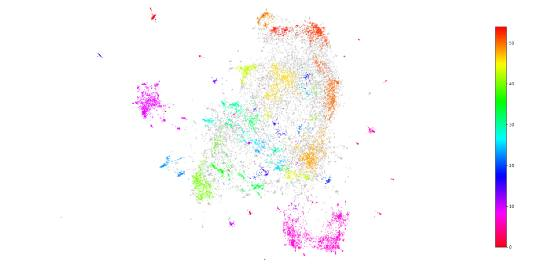
\includegraphics[scale=0.75]{hdbscan.jpg}
        \caption{Результат работы HDBSCAN}
        \label{fig:hdbscan}
    \end{figure}
\end{enumerate}
Формализуем HDBSCAN.
\begin{enumerate}
    \item Пусть $U_\epsilon(x)$ -- $\epsilon$-окрестность точки $x$, которая до этого не просматривалась. 
    \item Если точка $x$ содержит $minPts$ соседей (где $minPts$ и метрика, по которой находится расстояние между точками -- задаваемые гиперпараметры) или более, то образуется кластер
    \item Иначе точка помечается шумом. Возвращаемся к п.1.
    \item Повторяем, п.2-3 до момента, пока не получится связный кластер (между любыми соседями есть путь, как минимум, один);
    \item Повторяем п.1-4 для новой не просмотренной точки.
\end{enumerate}




\section{ПРАКТИЧЕСКАЯ ЧАСТЬ}
\vspace{-1.3cm}

\subsection{Используемые инструменты}

\begin{multicols}{3}
\begin{itemize}
 \item Python 3


 \item NumPy


 \item Pandas


 \item Matplotlib


 \item NLTK


 \item Spacy


 \item Scikit-learn


 \item TensorFlow


 \item JavaScript


 \item HTML и CSS


\item PyTorch


\item Bootstrap5


\item Flask


\item torchtext
\end{itemize}
\end{multicols}


\subsection{Экспериментальные результаты}
\subsubsection{Используемые данные}
\par
В задаче сентимент-анализа рассматривались датасеты для бинарной классификации (рецензии на кино с ресурса IMDB -- 50 тысяч строк и отзывы YELP -- 560 тысяч строк), для задачи классификации на три класса -- датасет комментариев социальной сети Twitter (74681 комментарий). В задаче тематического моделирования рассматривался предобработанный для обучения моделей классификации датасет IMDB. Для ансамблирования нейросетевых моделей сентимент-анализа были сконкатенированы датасеты Amazon и IMDB -- общее количество строк 3.625 миллиона.
% \newpage
\subsubsection{Одномерные сверточные нейронные сети}
В Таблице \ref{tab:cnn_result1} приведены метрики качества accuracy исследуемых архитектур на этапах обучения, валидации и тестирования моделей. 
%accuracy
\begin{center}
    \begin{table}[H]
        \centering
    \caption{Метрика accuracy на разных этапах обучения}

    \resizebox{\textwidth}{!}{\begin{tabular}{|c|ccccccccc|}
    \hline
    \multirow{3}{*}{Данные}                               & \multicolumn{9}{c|}{Модели}                                                                                                                                                                                                                                                                                         \\ \cline{2-10} 
                                                          & \multicolumn{3}{c|}{\begin{tabular}[c]{@{}c@{}}CNN \\ (1 слой)\end{tabular}}                     & \multicolumn{3}{c|}{\begin{tabular}[c]{@{}c@{}}CNN\\ (3 + 3 пулинг)\end{tabular}}                                & \multicolumn{3}{c|}{\begin{tabular}[c]{@{}c@{}}CNN\\ (5+5)\end{tabular}}                      \\ \cline{2-10} 
                                                          & \multicolumn{1}{c|}{Train}           & \multicolumn{1}{c|}{Val}    & \multicolumn{1}{c|}{Test}   & \multicolumn{1}{c|}{Train}          & \multicolumn{1}{c|}{Val}             & \multicolumn{1}{c|}{Test}           & \multicolumn{1}{c|}{Train}           & \multicolumn{1}{c|}{Val}             & Test            \\ \hline
    \begin{tabular}[c]{@{}c@{}}IMDB\\ (2)\end{tabular}    & \multicolumn{1}{c|}{\textbf{0.9996}} & \multicolumn{1}{c|}{0.8757} & \multicolumn{1}{c|}{0.889}  & \multicolumn{1}{c|}{0.997}          & \multicolumn{1}{c|}{\textbf{0.8994}} & \multicolumn{1}{c|}{0.8765}         & \multicolumn{1}{c|}{0.9963}          & \multicolumn{1}{c|}{0.8991}          & \textbf{0.8996} \\ \hline
    \begin{tabular}[c]{@{}c@{}}Twitter\\ (3)\end{tabular} & \multicolumn{1}{c|}{0.913}           & \multicolumn{1}{c|}{0,8338} & \multicolumn{1}{c|}{0.8447} & \multicolumn{1}{c|}{\textbf{0.945}} & \multicolumn{1}{c|}{0.8491}          & \multicolumn{1}{c|}{0.8312}         & \multicolumn{1}{c|}{0.93}            & \multicolumn{1}{c|}{\textbf{0.8542}} & \textbf{0.8771} \\ \hline
    \begin{tabular}[c]{@{}c@{}}Yelp\\ (2)\end{tabular}    & \multicolumn{1}{c|}{0.5312}          & \multicolumn{1}{c|}{0.5671} & \multicolumn{1}{c|}{0.5431} & \multicolumn{1}{c|}{0.5538}         & \multicolumn{1}{c|}{0.534}           & \multicolumn{1}{c|}{\textbf{0.613}} & \multicolumn{1}{c|}{\textbf{0.5652}} & \multicolumn{1}{c|}{\textbf{0.5843}} & 0.548           \\ \hline
    \multicolumn{1}{|l|}{Epochs}                          & \multicolumn{3}{c|}{5}                                                                           & \multicolumn{3}{c|}{5}                                                                                           & \multicolumn{3}{c|}{5}                                                                        \\ \hline
    \end{tabular}}
    \label{tab:cnn_result1}
\end{table}
\end{center}
%accuracy
Таблица \ref{tab:cnn_result2} содержит сравнение современных фреймворков для обучения нейронных сетей PyTorch и Tensorflow. 
В ней приведены длительности обучения моделей. 
%time
\begin{center}
\begin{table}[H]
    \centering
    \caption{Затраченное время на разных фреймворках}
    \resizebox{\textwidth}{!}{\begin{tabular}{|c|cccccc|c|}
    \hline
                                                          & \multicolumn{6}{c|}{Модели}                                                                                                                                                                         &                        \\ \hline
    \multirow{2}{*}{Данные}                               & \multicolumn{2}{c|}{\begin{tabular}[c]{@{}c@{}}CNN\\ (1 слой)\end{tabular}} & \multicolumn{2}{c|}{\begin{tabular}[c]{@{}c@{}}CNN \\ (3+3 пулинг)\end{tabular}} & \multicolumn{2}{c|}{CNN (5+5)}        & \multirow{2}{*}{Объем} \\ \cline{2-7}
                                                          & \multicolumn{1}{c|}{TF}              & \multicolumn{1}{c|}{PyTorch}         & \multicolumn{1}{c|}{TF}               & \multicolumn{1}{c|}{PyTorch}          & \multicolumn{1}{c|}{TF}     & PyTorch &                        \\ \hline
    \begin{tabular}[c]{@{}c@{}}IMDB\\ (2)\end{tabular}    & \multicolumn{1}{c|}{221}             & \multicolumn{1}{c|}{81}              & \multicolumn{1}{c|}{307}              & \multicolumn{1}{c|}{100}              & \multicolumn{1}{c|}{383}    & 132     & 50000                  \\ \hline
    \begin{tabular}[c]{@{}c@{}}Twitter\\ (3)\end{tabular} & \multicolumn{1}{c|}{385}             & \multicolumn{1}{c|}{313}             & \multicolumn{1}{c|}{497}              & \multicolumn{1}{c|}{433}              & \multicolumn{1}{c|}{754}    & 532     & 75000                  \\ \hline
    \begin{tabular}[c]{@{}c@{}}Yelp\\ (2)\end{tabular}    & \multicolumn{1}{c|}{100421}          & \multicolumn{1}{c|}{120212}          & \multicolumn{1}{c|}{220053}           & \multicolumn{1}{c|}{189429}           & \multicolumn{1}{c|}{315371} & 435341  & 560000                 \\ \hline
    \end{tabular}}
    \label{tab:cnn_result2}
    \end{table}
\end{center}
%time
На рис. \ref{fig:cnn_batch} и рис. \ref{fig:cnn_optimizer} изображены поведения ошибки и метрики качества в зависимости от выбора размера пакета и оптимизатора, соответственно.
\begin{figure}[H]
    \centering
    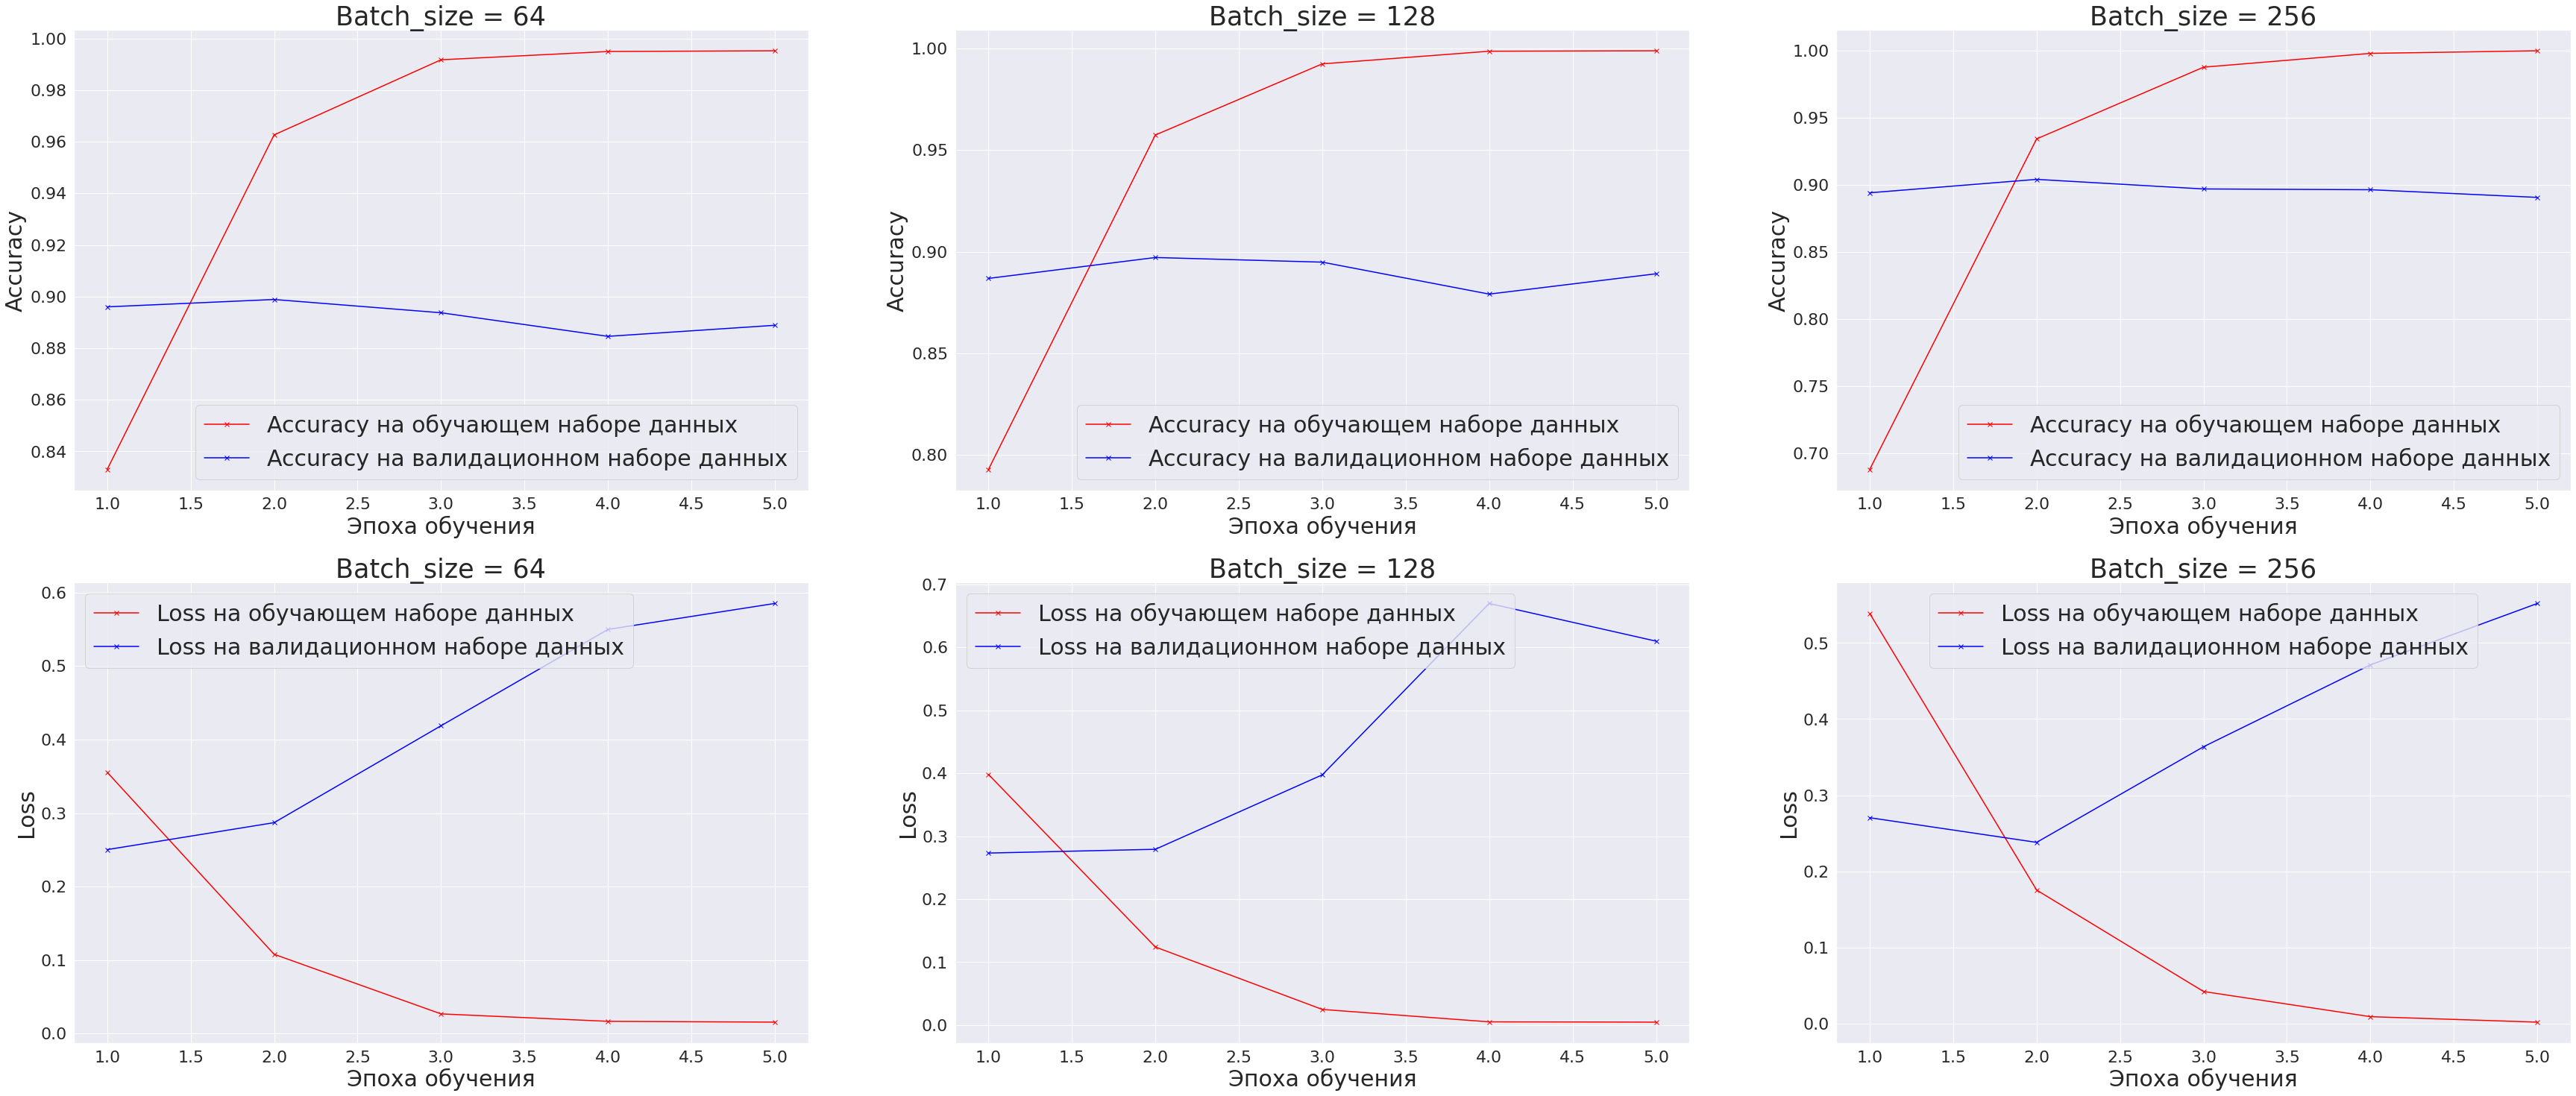
\includegraphics[scale=0.14]{cnn_batch.png}
    \caption{Поведение accuracy и loss в зависимости от batch size}
    \label{fig:cnn_batch}
\end{figure}
\begin{figure}[H]
    \centering
    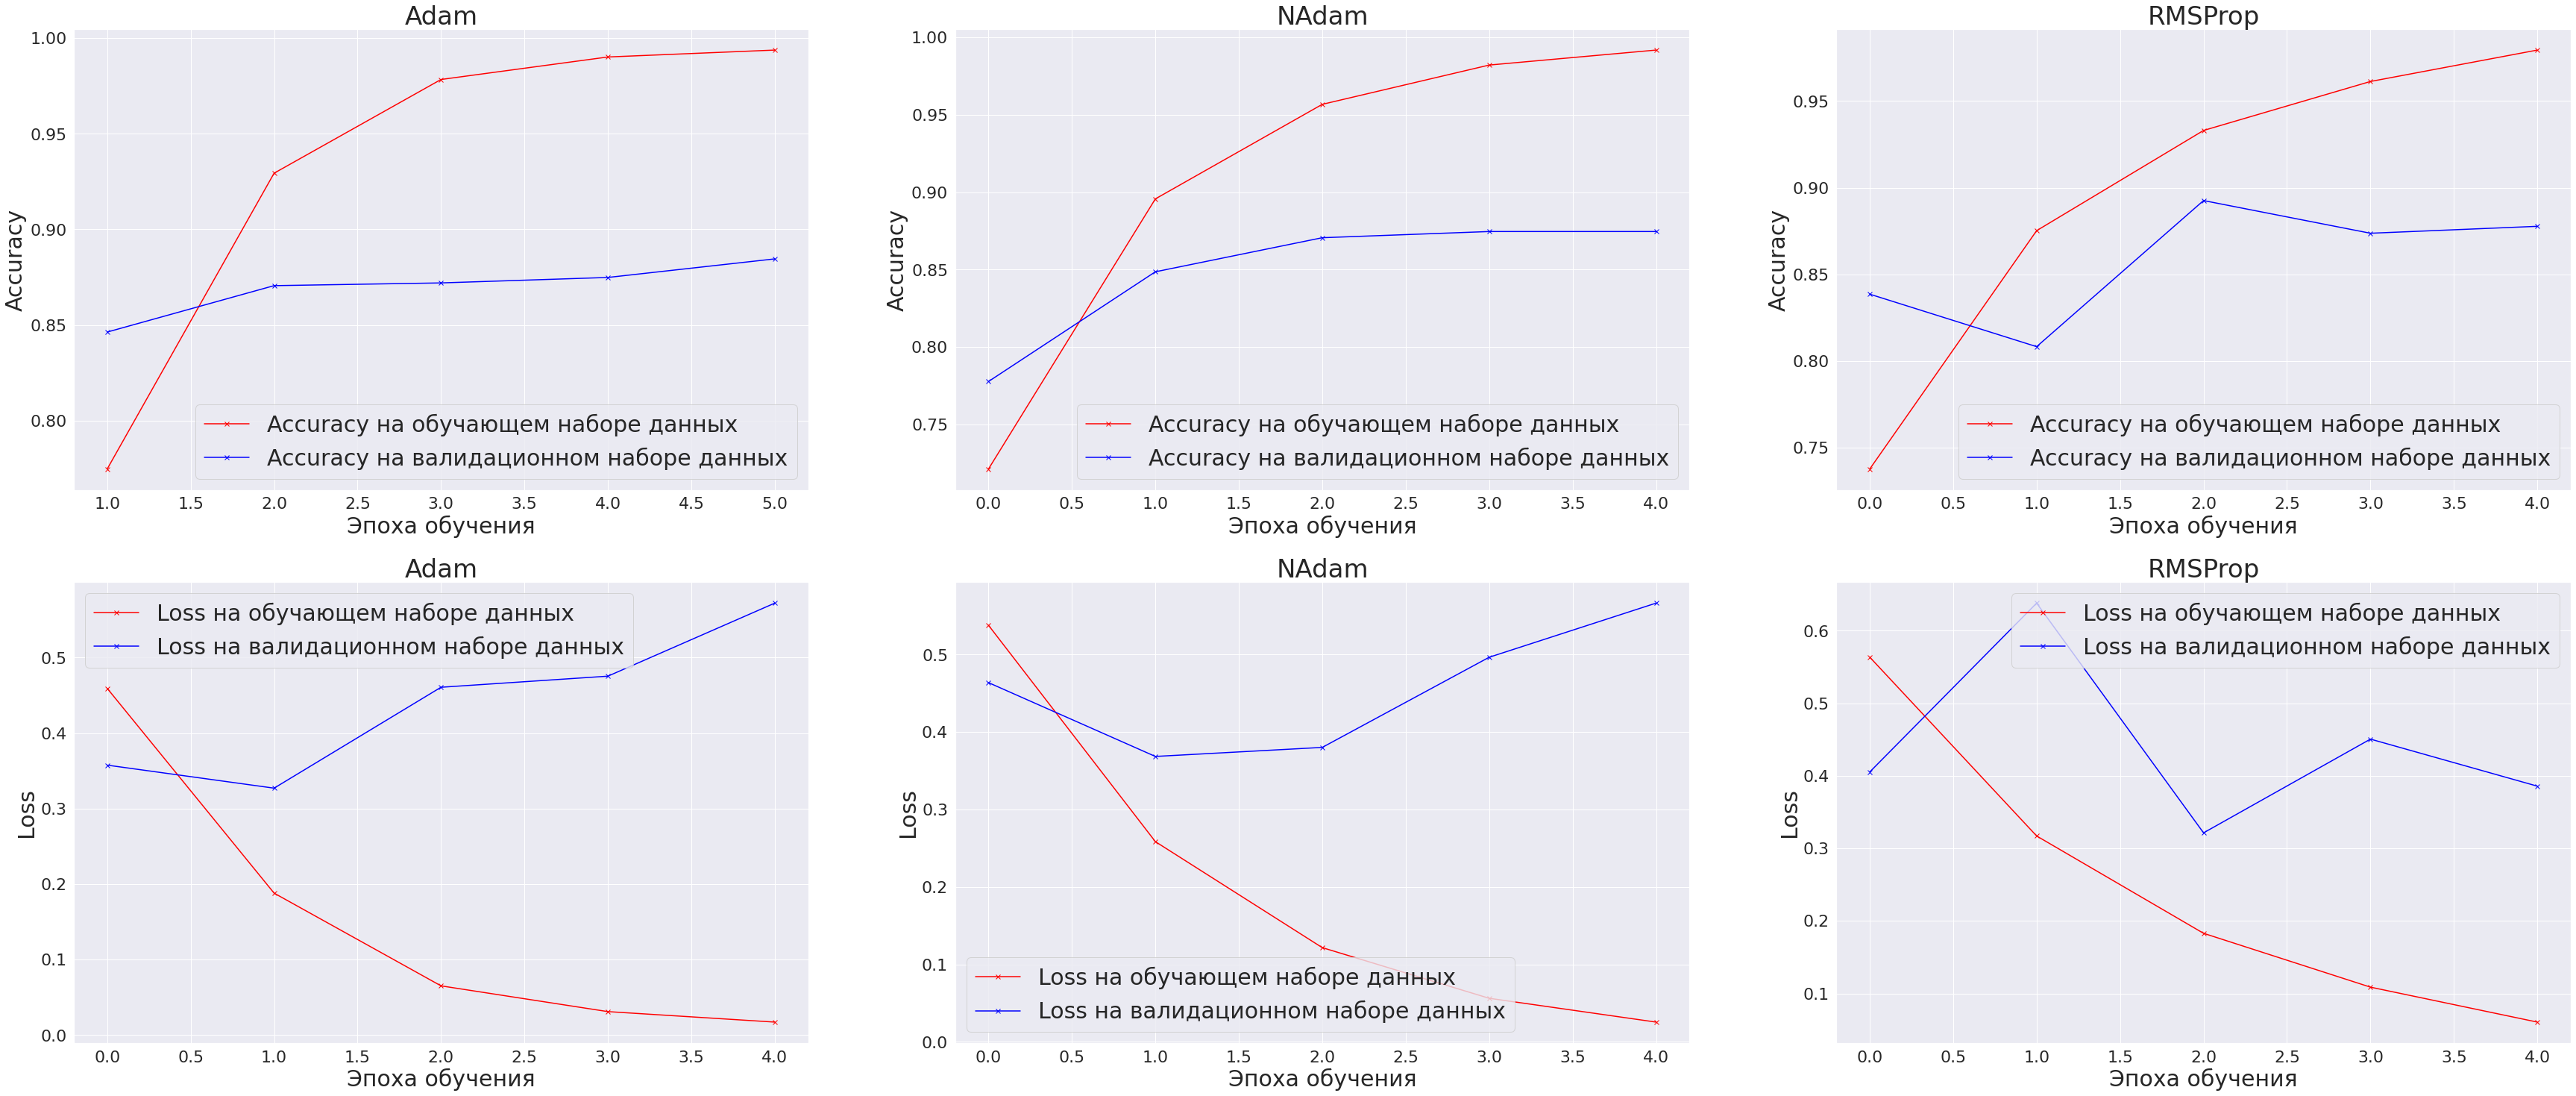
\includegraphics[scale=0.14]{cnn_optim.png}
    \caption{Поведение accuracy и loss в зависимости от выбора оптимизатора}
    \label{fig:cnn_optimizer}
\end{figure}
\subsubsection{Рекуррентные нейронные сети}
В Таблице \ref{tab:lstm_result1} приведены метрики качества accuracy исследуемых архитектур на этапах обучения, валидации и тестирования моделей. 
%accuracy lstm
\begin{center}
\begin{table}[H]
    \centering
    \caption{Метрика accuracy на разных этапах обучения}
    \resizebox{\textwidth}{!}{\begin{tabular}{|c|ccccccccc|}
    \hline
    \multirow{3}{*}{Данные}                               & \multicolumn{9}{c|}{Модели}                                                                                                                                                                                                                                                                                                           \\ \cline{2-10} 
                                                          & \multicolumn{3}{c|}{\begin{tabular}[c]{@{}c@{}}LSTM\\ (1 блок)\end{tabular}}                                      & \multicolumn{3}{c|}{\begin{tabular}[c]{@{}c@{}}LSTM\\ (2 блока)\end{tabular}}                            & \multicolumn{3}{c|}{\begin{tabular}[c]{@{}c@{}}CNN + LSTM\\ (1 слой + 1 пулинг + 1 блок)\end{tabular}} \\ \cline{2-10} 
                                                          & \multicolumn{1}{c|}{Train}           & \multicolumn{1}{c|}{Val}             & \multicolumn{1}{c|}{Test}           & \multicolumn{1}{c|}{Train}  & \multicolumn{1}{c|}{Val}             & \multicolumn{1}{c|}{Test}           & \multicolumn{1}{c|}{Train}              & \multicolumn{1}{c|}{Val}                & Test               \\ \hline
    \begin{tabular}[c]{@{}c@{}}IMDB\\ (2)\end{tabular}    & \multicolumn{1}{c|}{0.9968}          & \multicolumn{1}{c|}{0.8809}          & \multicolumn{1}{c|}{0.8573}         & \multicolumn{1}{c|}{0.9533} & \multicolumn{1}{c|}{\textbf{0.8834}} & \multicolumn{1}{c|}{0.8673}         & \multicolumn{1}{c|}{\textbf{0.9982}}    & \multicolumn{1}{c|}{0.88}               & \textbf{0.8765}    \\ \hline
    \begin{tabular}[c]{@{}c@{}}Twitter\\ (3)\end{tabular} & \multicolumn{1}{c|}{\textbf{0.855}}  & \multicolumn{1}{c|}{0.84}            & \multicolumn{1}{c|}{0.778}          & \multicolumn{1}{c|}{0.8431} & \multicolumn{1}{c|}{0.8393}          & \multicolumn{1}{c|}{\textbf{0.841}} & \multicolumn{1}{c|}{0.815}              & \multicolumn{1}{c|}{\textbf{0.8542}}    & 0.8175             \\ \hline
    \begin{tabular}[c]{@{}c@{}}Yelp\\ (2)\end{tabular}    & \multicolumn{1}{c|}{\textbf{0.9172}} & \multicolumn{1}{c|}{\textbf{0.9472}} & \multicolumn{1}{c|}{\textbf{0.945}} & \multicolumn{1}{c|}{0.91}   & \multicolumn{1}{c|}{0.864}           & \multicolumn{1}{c|}{0.8621}         & \multicolumn{1}{c|}{-}                  & \multicolumn{1}{c|}{\textbf{-}}         & -                  \\ \hline
    \multicolumn{1}{|l|}{Epochs}                          & \multicolumn{3}{c|}{13}                                                                                           & \multicolumn{3}{c|}{10}                                                                                  & \multicolumn{3}{c|}{10}                                                                                \\ \hline
    \end{tabular}}
    \label{tab:lstm_result1}
    \end{table}
\end{center}
%accuracy lstm
Таблица \ref{tab:lstm_result2} содержит сравнение современных фреймворков для обучения нейронных сетей PyTorch и Tensorflow. 
%time lstm
\begin{center}
\begin{table}[H]
    \centering
    \caption{Затраченное время на разных фреймворках}
    \resizebox{\textwidth}{!}{\begin{tabular}{|c|cccccc|c|}
    \hline
                                                          & \multicolumn{6}{c|}{Модели}                                                                                                                                                                        &                        \\ \hline
    \multirow{2}{*}{Данные}                               & \multicolumn{2}{c|}{\begin{tabular}[c]{@{}c@{}}LSTM\\ (1 блок)\end{tabular}} & \multicolumn{2}{c|}{\begin{tabular}[c]{@{}c@{}}LSTM\\ (2 блока)\end{tabular}} & \multicolumn{2}{c|}{LSTM + CNN}     & \multirow{2}{*}{Объем} \\ \cline{2-7}
                                                          & \multicolumn{1}{c|}{TF}              & \multicolumn{1}{c|}{PyTorch}          & \multicolumn{1}{c|}{TF}               & \multicolumn{1}{c|}{PyTorch}          & \multicolumn{1}{c|}{TF}   & PyTorch &                        \\ \hline
    \begin{tabular}[c]{@{}c@{}}IMDB\\ (2)\end{tabular}    & \multicolumn{1}{c|}{225}             & \multicolumn{1}{c|}{201}              & \multicolumn{1}{c|}{8400}             & \multicolumn{1}{c|}{8513}             & \multicolumn{1}{c|}{1800} & 1680    & 50000                  \\ \hline
    \begin{tabular}[c]{@{}c@{}}Twitter\\ (3)\end{tabular} & \multicolumn{1}{c|}{541}             & \multicolumn{1}{c|}{650}              & \multicolumn{1}{c|}{28326}            & \multicolumn{1}{c|}{31652}            & \multicolumn{1}{c|}{3366} & 3254    & 75000                  \\ \hline
    \begin{tabular}[c]{@{}c@{}}Yelp\\ (2)\end{tabular}    & \multicolumn{1}{c|}{432002}          & \multicolumn{1}{c|}{542331}           & \multicolumn{1}{c|}{479032}           & \multicolumn{1}{c|}{482151}           & \multicolumn{1}{c|}{-}    & -       & 560000                 \\ \hline
    \end{tabular}}
    \label{tab:lstm_result2}
    \end{table}
\end{center}
%time lstm
На рис. \ref{fig:lstm_batch} и рис. \ref{fig:cnn_optimizer} изображены поведения ошибки и метрики качества в зависимости от выбора размера пакета и оптимизатора, соответственно.
\begin{figure}[H]
    \centering
    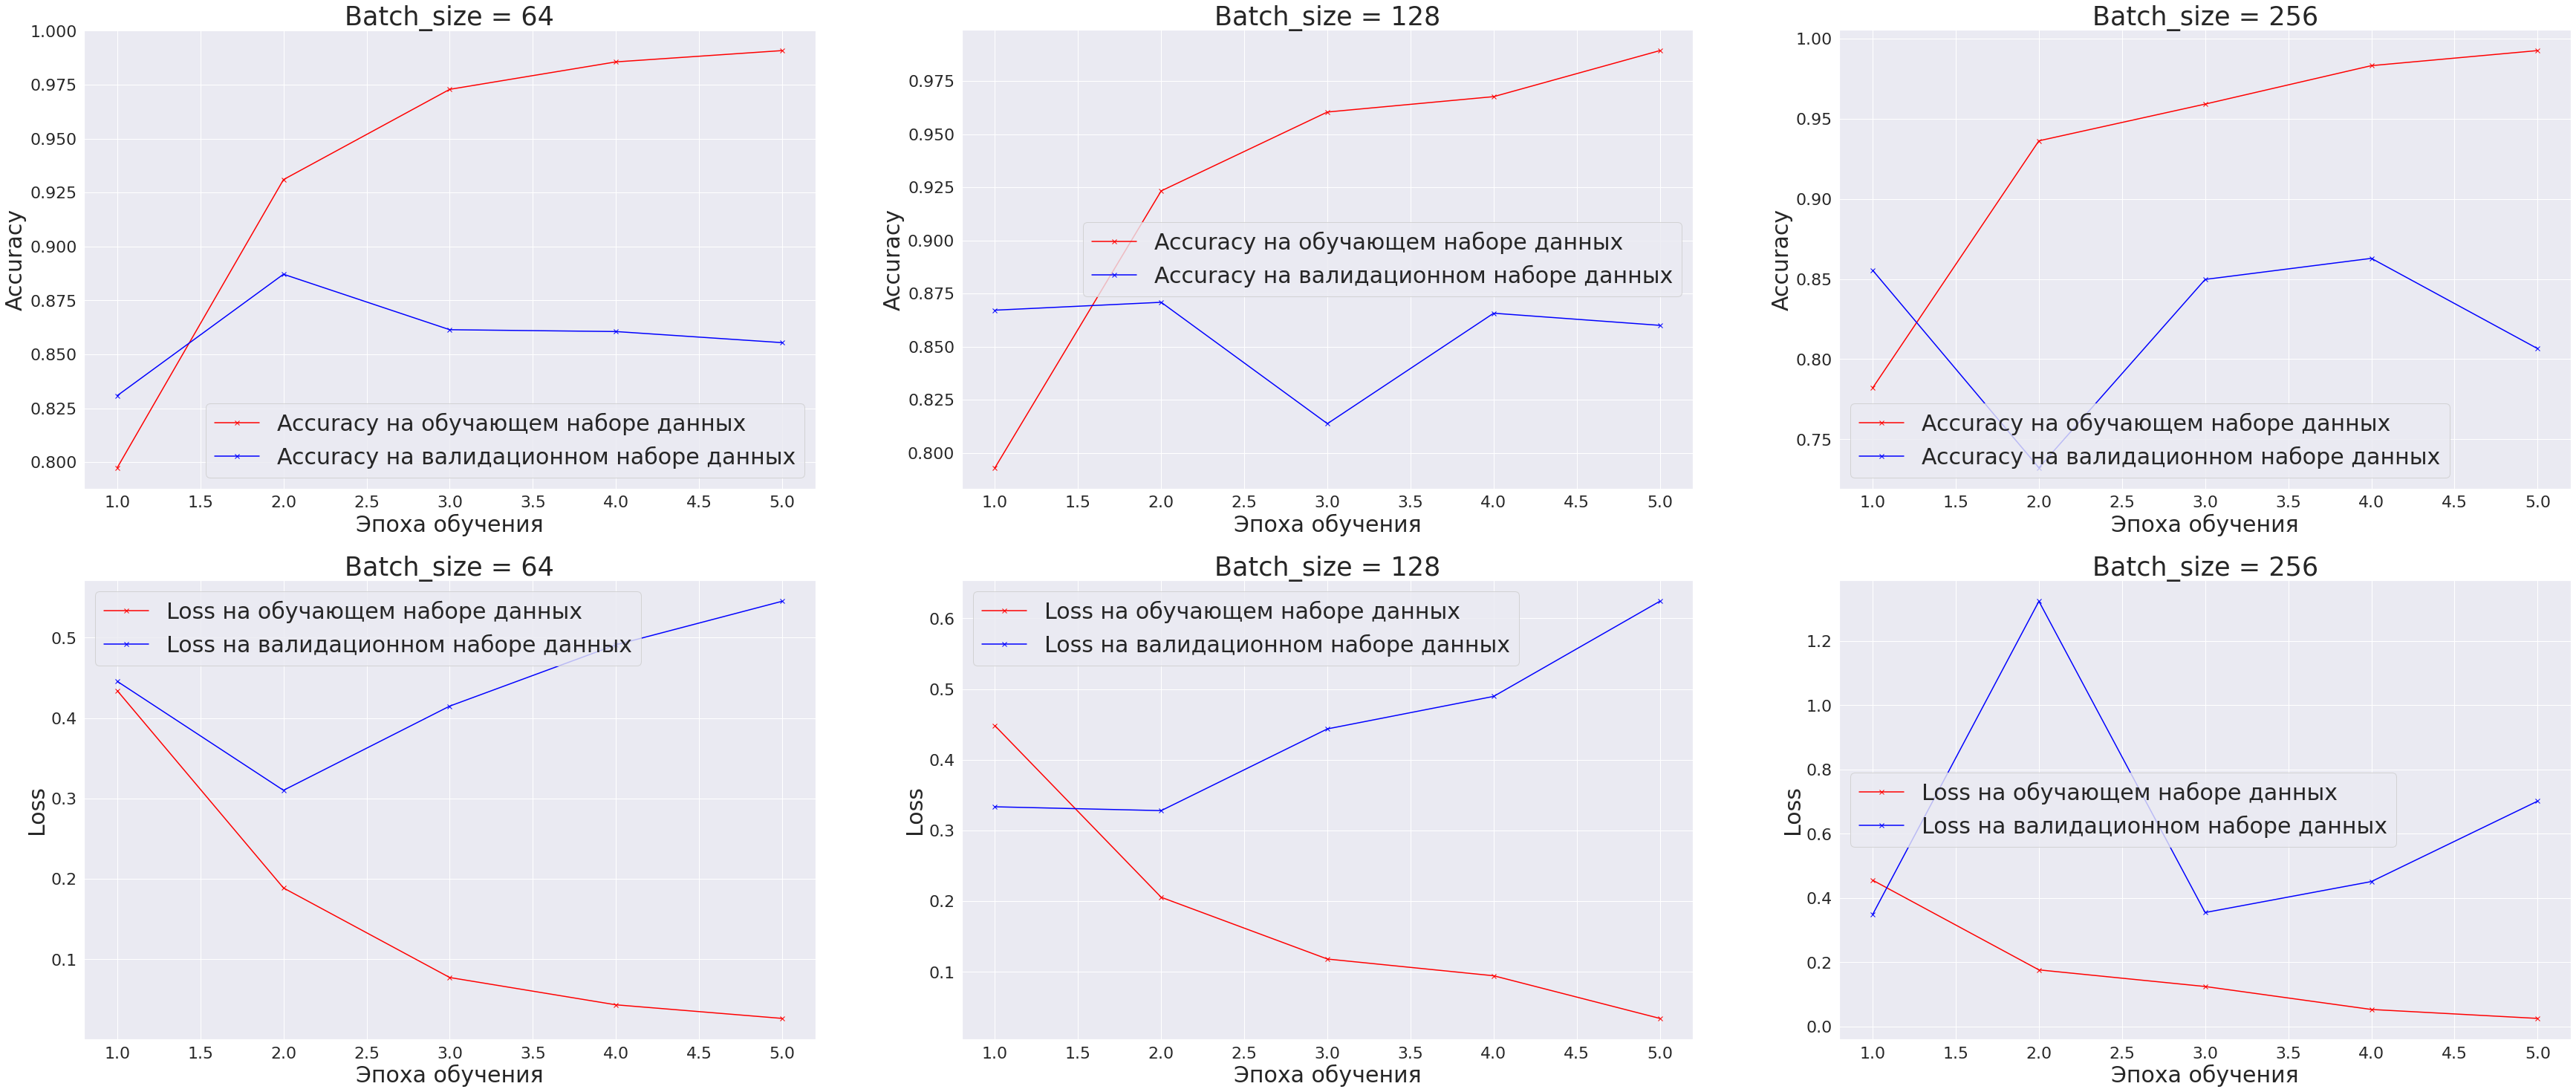
\includegraphics[scale=0.14]{lstm_batch.png}
    \caption{Поведение accuracy и loss в зависимости от batch size}
    \label{fig:lstm_batch}
\end{figure}
\begin{figure}[H]
    \centering
    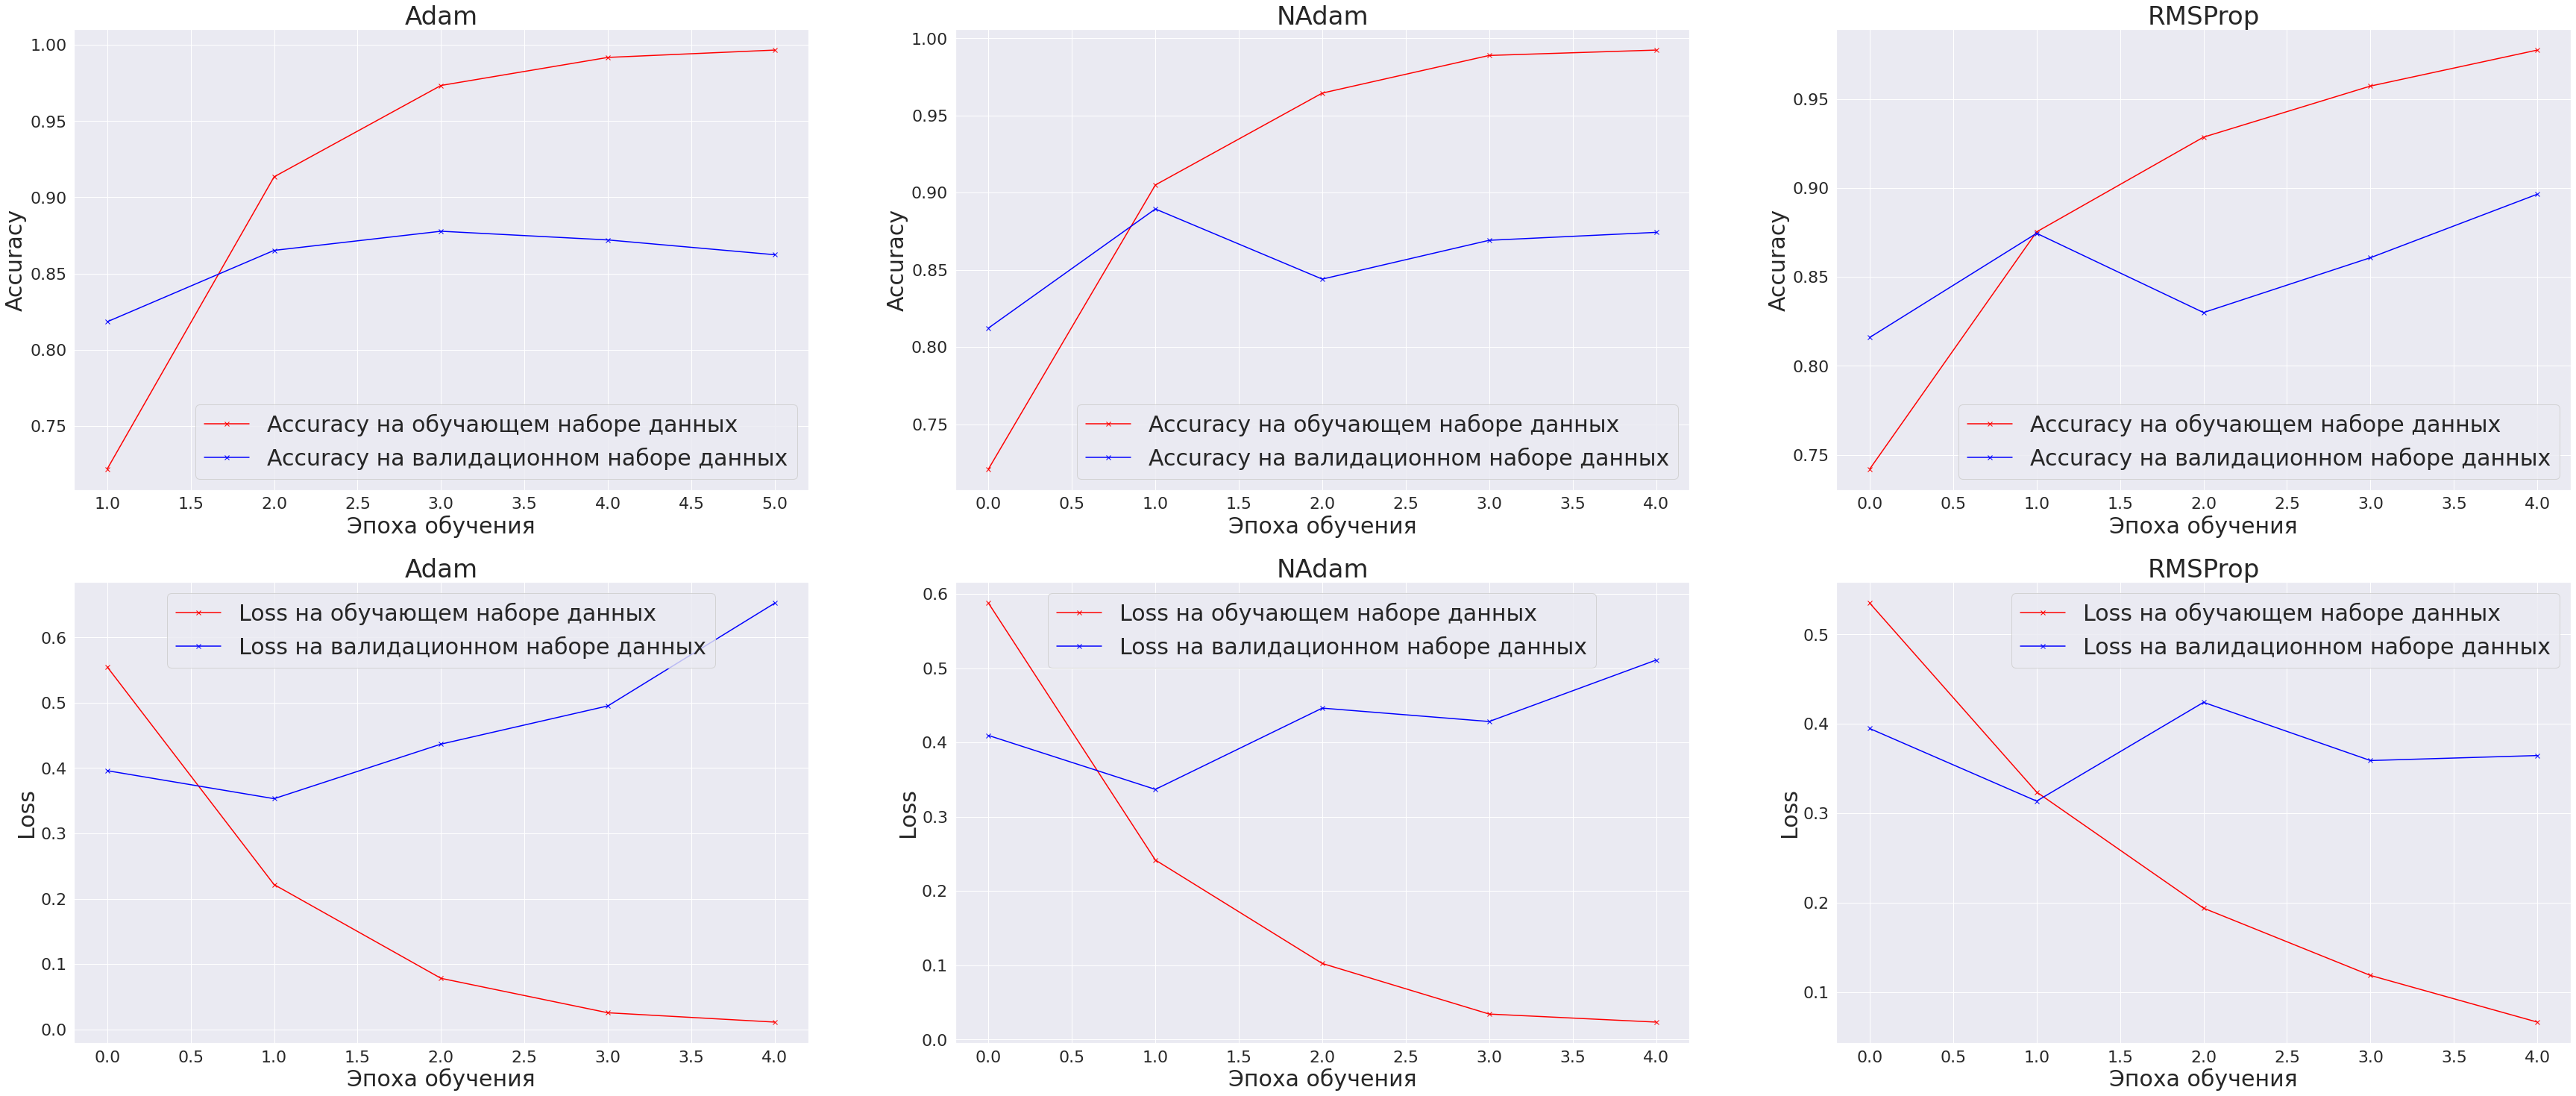
\includegraphics[scale=0.14]{lstm_optim.png}
    \caption{Поведение accuracy и loss в зависимости от выбора оптимизатора}
    \label{fig:lstm_optimizer}
\end{figure}
В Таблице \ref{tab:gru_result1} приведены метрики качества accuracy исследуемых архитектур на этапах обучения, валидации и тестирования моделей. 
%accuracy gru
\begin{center}
    % Please add the following required packages to your document preamble:
% \usepackage{multirow}
\begin{table}[H]
    \centering
    \caption{Метрика accuracy на разных этапах обучения}
    \resizebox{\textwidth}{!}{\begin{tabular}{|c|ccccccccc|}
    \hline
    \multirow{3}{*}{Данные}                               & \multicolumn{9}{c|}{Модели}                                                                                                                                                                                                                                                                                          \\ \cline{2-10} 
                                                          & \multicolumn{3}{c|}{\begin{tabular}[c]{@{}c@{}}GRU\\ (1 блок)\end{tabular}}                                        & \multicolumn{3}{c|}{\begin{tabular}[c]{@{}c@{}}GRU\\ (2 блока)\end{tabular}}            & \multicolumn{3}{c|}{\begin{tabular}[c]{@{}c@{}}CNN + GRU\\ (5 слой + 5 пулинг + 1 блок)\end{tabular}} \\ \cline{2-10} 
                                                          & \multicolumn{1}{c|}{Train}           & \multicolumn{1}{c|}{Val}             & \multicolumn{1}{c|}{Test}            & \multicolumn{1}{c|}{Train}  & \multicolumn{1}{c|}{Val}    & \multicolumn{1}{c|}{Test}   & \multicolumn{1}{c|}{Train}              & \multicolumn{1}{c|}{Val}               & Test               \\ \hline
    \begin{tabular}[c]{@{}c@{}}IMDB\\ (2)\end{tabular}    & \multicolumn{1}{c|}{0.9751}          & \multicolumn{1}{c|}{\textbf{0.9612}} & \multicolumn{1}{c|}{\textbf{0.9353}} & \multicolumn{1}{c|}{0.9903} & \multicolumn{1}{c|}{0.8764} & \multicolumn{1}{c|}{0.8931} & \multicolumn{1}{c|}{\textbf{0.9969}}    & \multicolumn{1}{c|}{0.8851}            & 0.9185             \\ \hline
    \begin{tabular}[c]{@{}c@{}}Twitter\\ (3)\end{tabular} & \multicolumn{1}{c|}{0.8788}          & \multicolumn{1}{c|}{0.8338}          & \multicolumn{1}{c|}{0.8447}          & \multicolumn{1}{c|}{0.9937} & \multicolumn{1}{c|}{0.9605} & \multicolumn{1}{c|}{0.9574} & \multicolumn{1}{c|}{0.93}               & \multicolumn{1}{c|}{\textbf{0.872}}    & \textbf{0.8771}    \\ \hline
    \begin{tabular}[c]{@{}c@{}}Yelp\\ (2)\end{tabular}    & \multicolumn{1}{c|}{\textbf{0.9670}} & \multicolumn{1}{c|}{\textbf{0.9562}} & \multicolumn{1}{c|}{\textbf{0.9459}} & \multicolumn{1}{c|}{0.954}  & \multicolumn{1}{c|}{0.943}  & \multicolumn{1}{c|}{0.9126} & \multicolumn{1}{c|}{-}                  & \multicolumn{1}{c|}{\textbf{-}}        & -                  \\ \hline
    \multicolumn{1}{|l|}{Epochs}                          & \multicolumn{3}{c|}{5}                                                                                             & \multicolumn{3}{c|}{5}                                                                  & \multicolumn{3}{c|}{5}                                                                                \\ \hline
    \end{tabular}}
    \label{tab:gru_result1}
    \end{table}
\end{center}
%accuracy gru
Таблица \ref{tab:gru_result2} содержит сравнение современных фреймворков для обучения нейронных сетей PyTorch и Tensorflow. 
В ней приведены длительности обучения моделей. 
%time gru
\begin{center}
    \begin{table}[H]
        \caption{Затраченное время на разных фреймворках}
        \resizebox{\textwidth}{!}{\begin{tabular}{|c|cccccc|c|}
        \hline
                                                              & \multicolumn{6}{c|}{Модели}                                                                                                                                                                      &                        \\ \hline
        \multirow{2}{*}{Данные}                               & \multicolumn{2}{c|}{\begin{tabular}[c]{@{}c@{}}GRU\\ (1 блок)\end{tabular}} & \multicolumn{2}{c|}{\begin{tabular}[c]{@{}c@{}}GRU \\ (2 блока)\end{tabular}} & \multicolumn{2}{c|}{GRU + CNN}     & \multirow{2}{*}{Объем} \\ \cline{2-7}
                                                              & \multicolumn{1}{c|}{TF}              & \multicolumn{1}{c|}{PyTorch}         & \multicolumn{1}{c|}{TF}               & \multicolumn{1}{c|}{PyTorch}          & \multicolumn{1}{c|}{TF}  & PyTorch &                        \\ \hline
        \begin{tabular}[c]{@{}c@{}}IMDB\\ (2)\end{tabular}    & \multicolumn{1}{c|}{189}             & \multicolumn{1}{c|}{204}             & \multicolumn{1}{c|}{569}              & \multicolumn{1}{c|}{642}              & \multicolumn{1}{c|}{244} & 183     & 50000                  \\ \hline
        \begin{tabular}[c]{@{}c@{}}Twitter\\ (3)\end{tabular} & \multicolumn{1}{c|}{546}             & \multicolumn{1}{c|}{498}             & \multicolumn{1}{c|}{759}              & \multicolumn{1}{c|}{802}              & \multicolumn{1}{c|}{650} & 663     & 75000                  \\ \hline
        \begin{tabular}[c]{@{}c@{}}Yelp\\ (2)\end{tabular}    & \multicolumn{1}{c|}{433200}          & \multicolumn{1}{c|}{454233}          & \multicolumn{1}{c|}{679036}           & \multicolumn{1}{c|}{592431}           & \multicolumn{1}{c|}{-}   & -       & 560000                 \\ \hline
        \end{tabular}}
        \label{tab:gru_result2}
        \end{table}
\end{center}
%time gru
На рис. \ref{fig:gru_batch} и рис. \ref{fig:gru_optimizer} изображены поведения ошибки и метрики качества в зависимости от выбора размера пакета и оптимизатора, соответственно.
\begin{figure}[H]
    \centering
    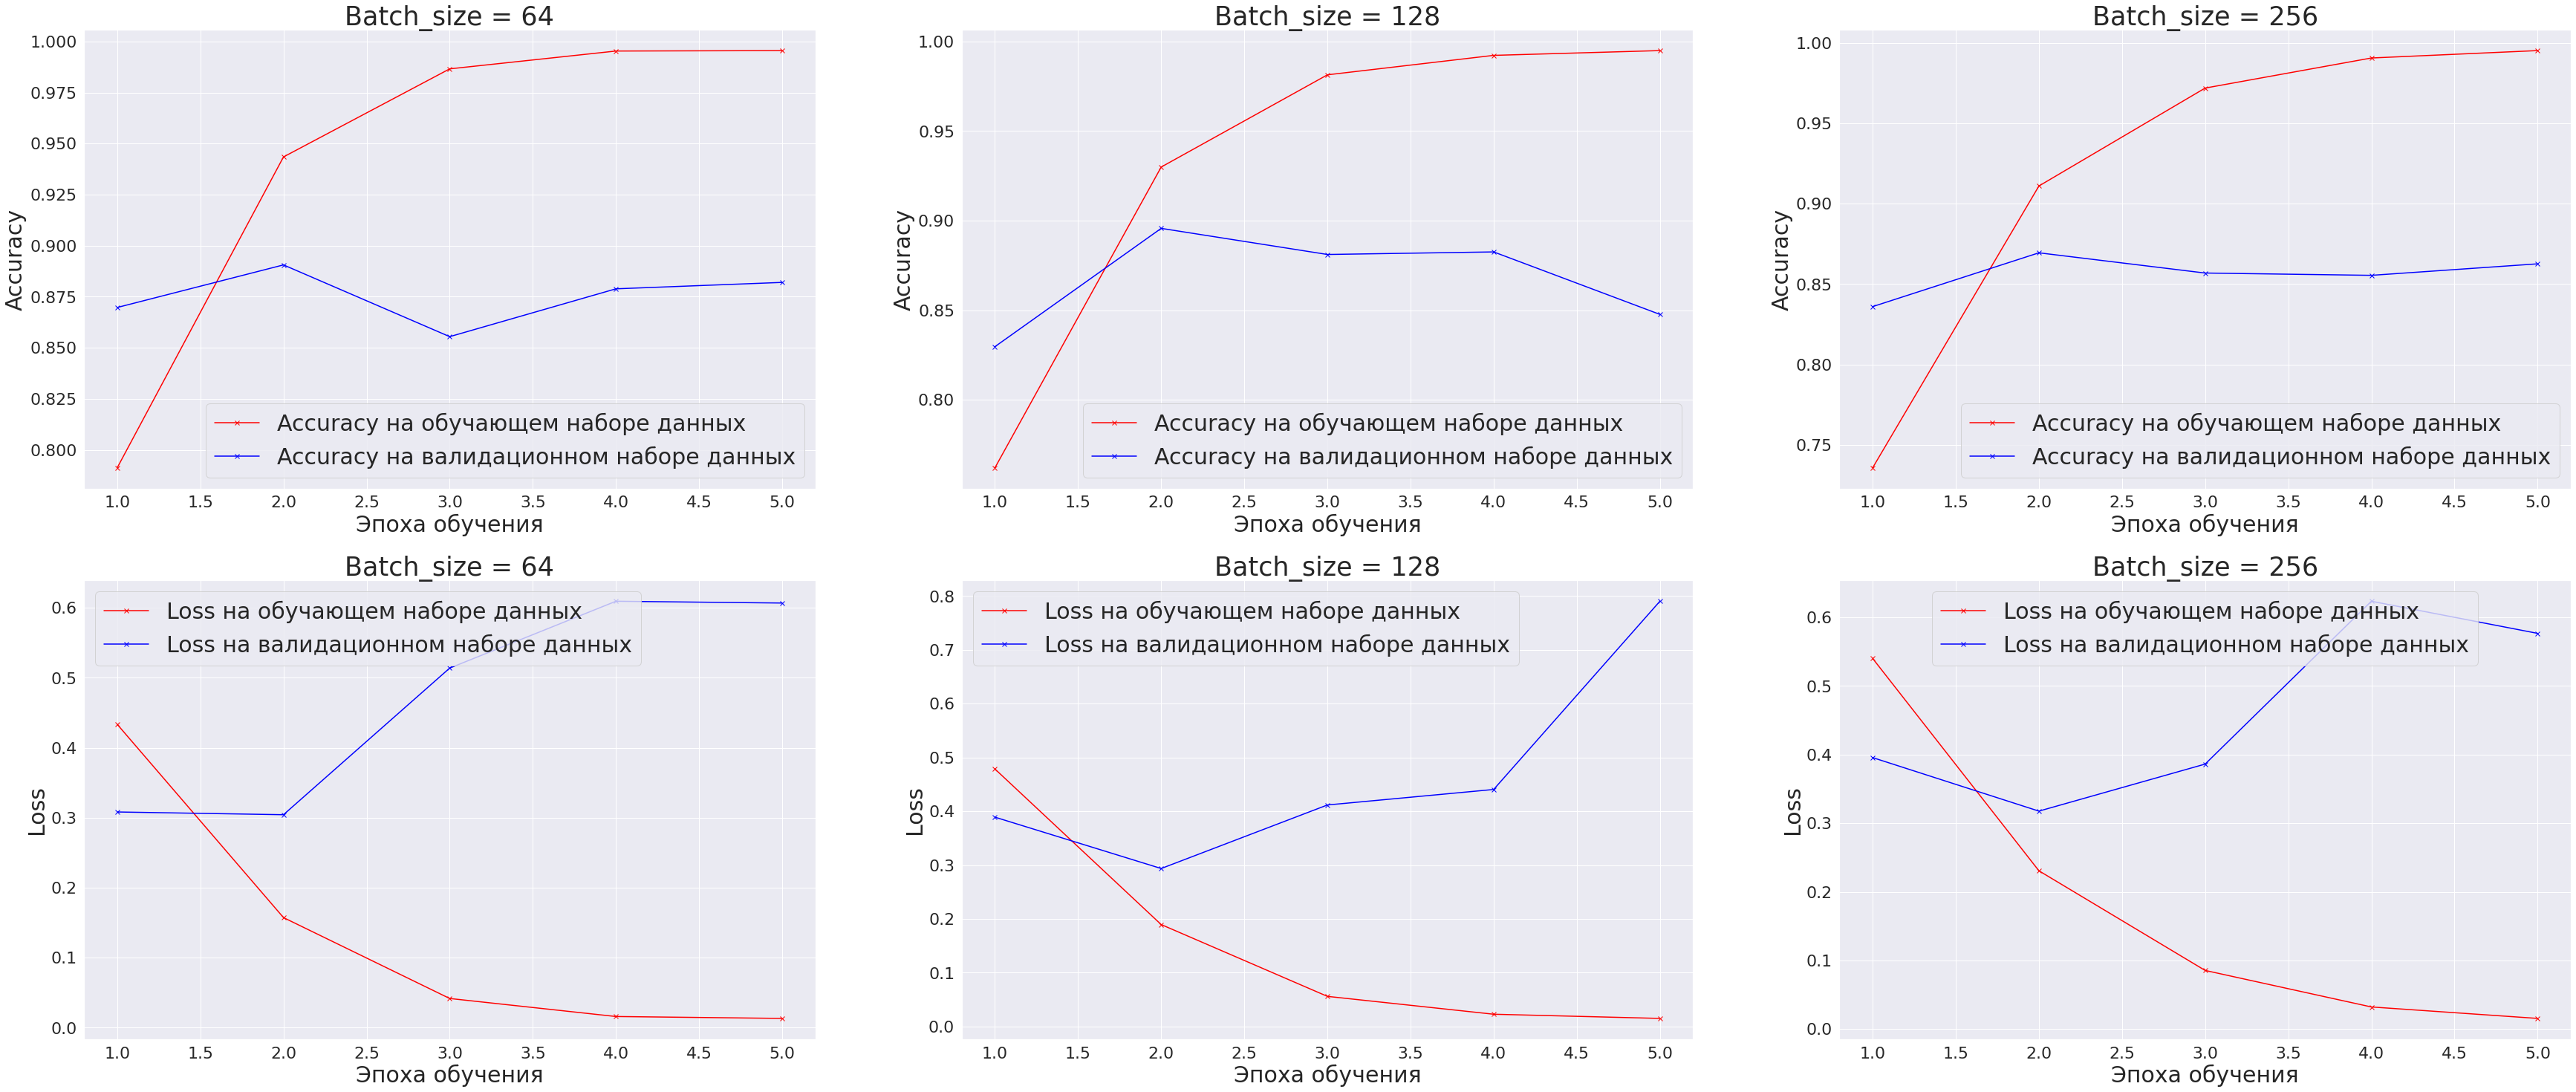
\includegraphics[scale=0.14]{gru_batch.png}
    \caption{Поведение accuracy и loss в зависимости от batch size}
    \label{fig:gru_batch}
\end{figure}
\begin{figure}[H]
    \centering
    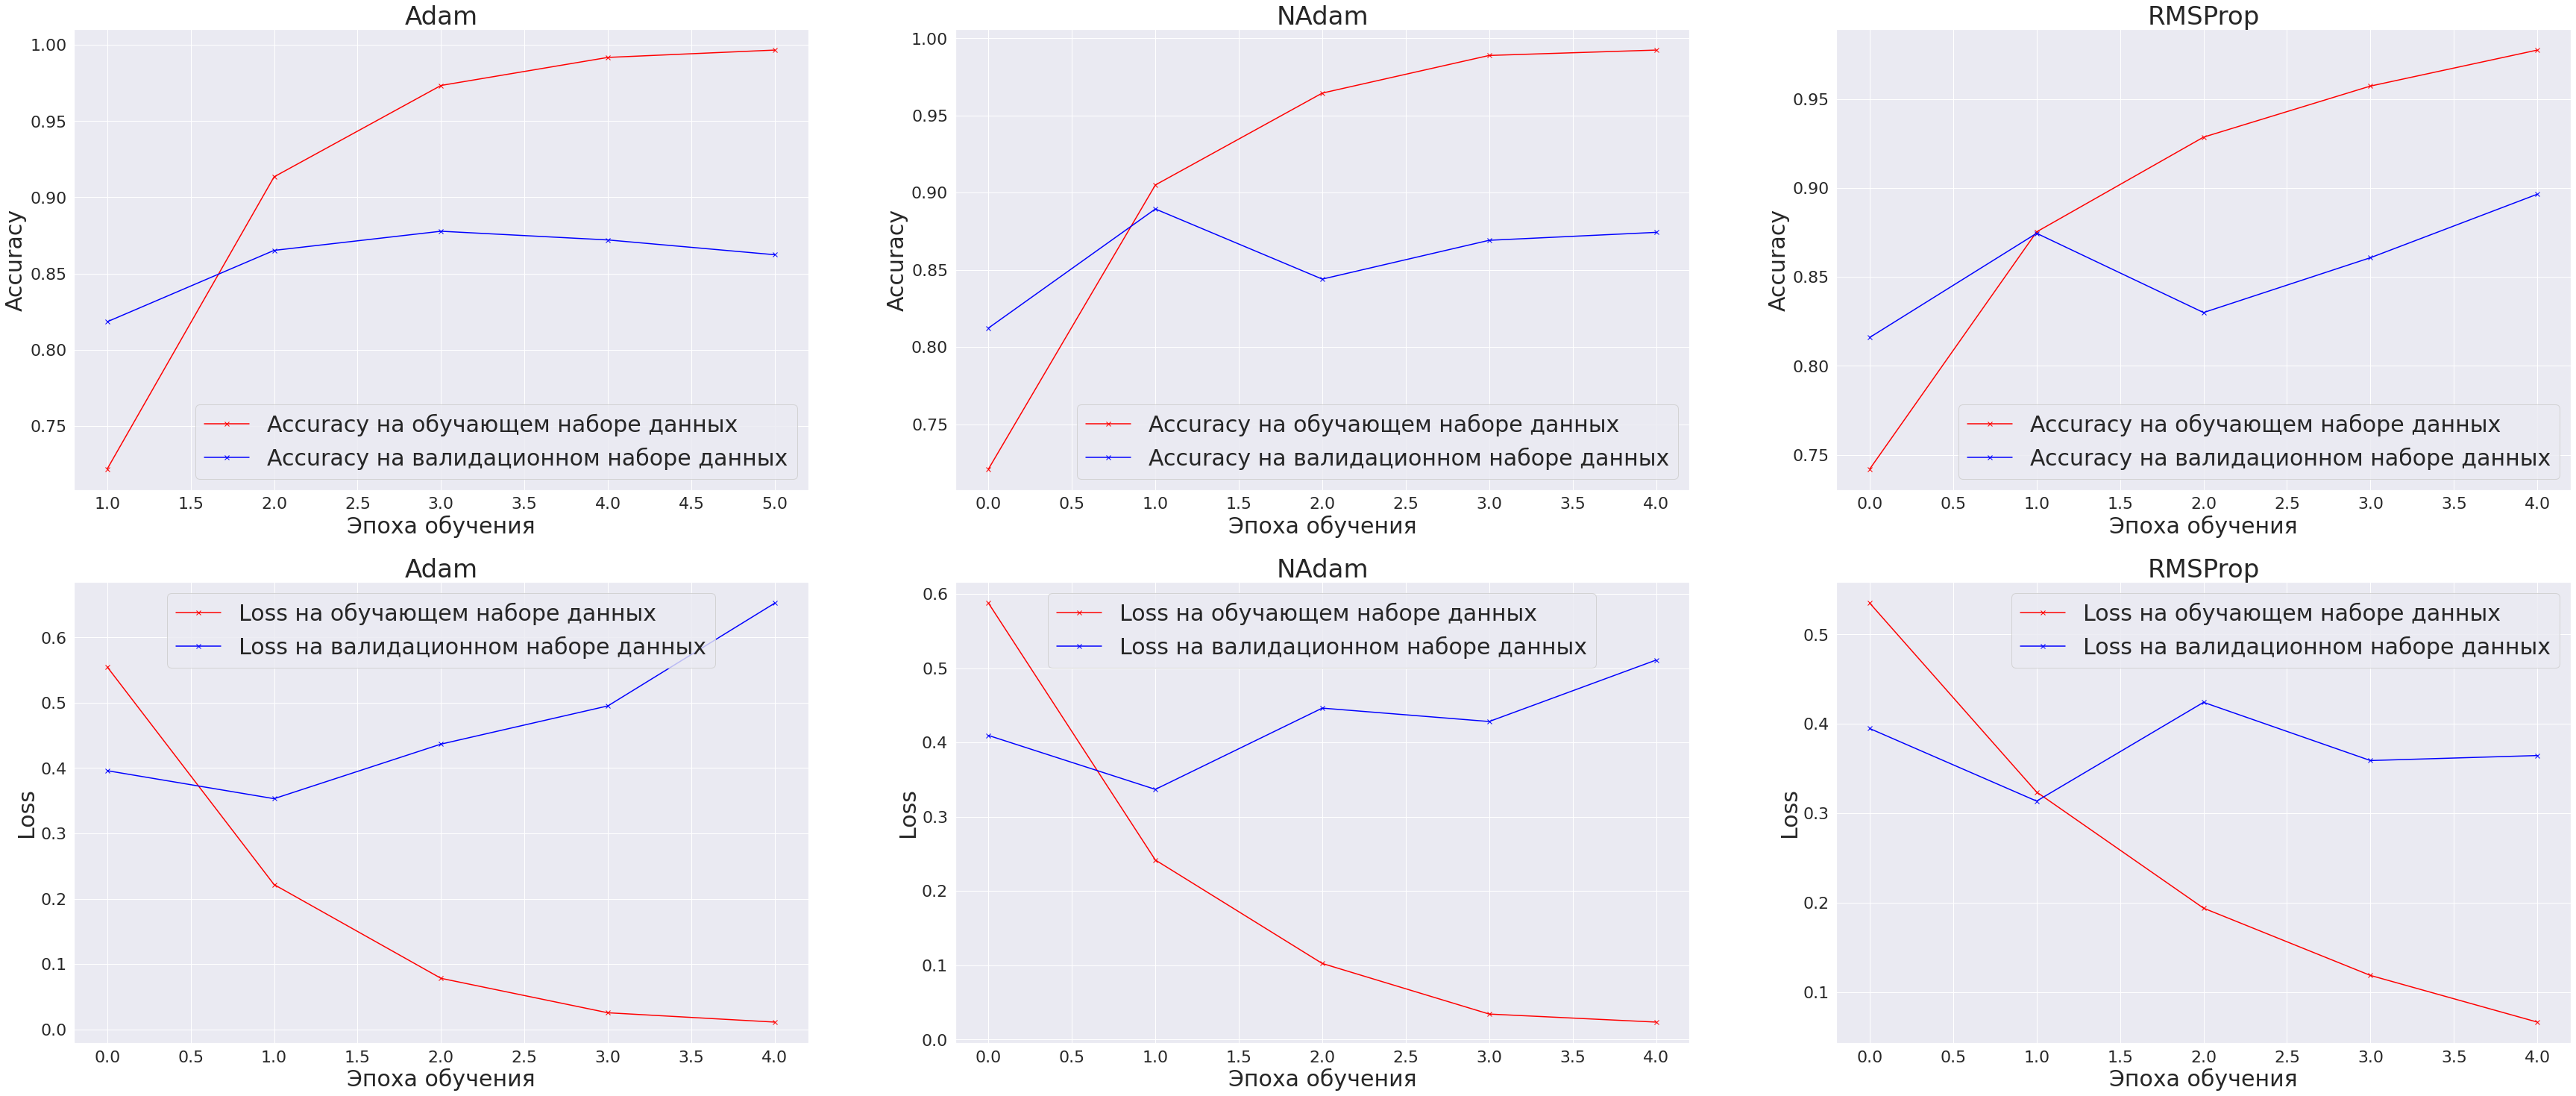
\includegraphics[scale=0.14]{gru_optim.png}
    \caption{Поведение accuracy и loss в зависимости от выбора оптимизатора}
    \label{fig:gru_optimizer}
\end{figure}
Embedding-слой, как и предполагалось, показал лучший результат по сравнению с предобученными моделями Word2Vec (Таблица \ref{tab:embeddings}), однако, разница невелика, поэтому можно сделать вывод, что в промышленной разработке следует использовать последний в силу большего по объемам латентного словаря (если нет ограничений по памяти).
    \begin{table}[H]
    \begin{center}
\caption{Сравнение различных векторных представлений слов}
\scalebox{0.87}[0.87]{\begin{tabular}{|l|ccc|}
\hline
                                                               & \multicolumn{3}{c|}{Модели}                                                                                                               \\ \cline{2-4} 
\multirow{-2}{*}{Эмбеддинги}                                   & \multicolumn{1}{c|}{CNN}                            & \multicolumn{1}{c|}{LSTM}                          & GRU                            \\ \hline
W2V CBOW                                                       & \multicolumn{1}{c|}{0.8991}                         & \multicolumn{1}{c|}{0.88}                          & 0.9353                         \\ \hline
W2V Skip-gram                                                  & \multicolumn{1}{c|}{\textbf{0.8771}} & \multicolumn{1}{c|}{\textbf{0.841}} & \textbf{0.9574} \\ \hline
\begin{tabular}[c]{@{}l@{}}Trainable \\ embedding\end{tabular} & \multicolumn{1}{c|}{0.9012}                         & \multicolumn{1}{c|}{0.9172}                        & 0.9562                         \\ \hline
\end{tabular}}
\label{tab:embeddings}
\end{center}
\end{table}
\subsubsection{Приемы мета-моделирования}
Полученные обученные модели показывают хорошие результаты, однако их можно дополнительно улучшить с помощью технологий стэкинга. Идея заключается в создании метамодели, которая будет по результатам мета-признаков моделей давать конечное предсказание. Обучение моделей для создания мета-модели проходило по принципу Stratified K-Foldation с сохранением балансировки классов (рис. \ref{fig:kfold}).  
\begin{figure}[H]
    \centering
    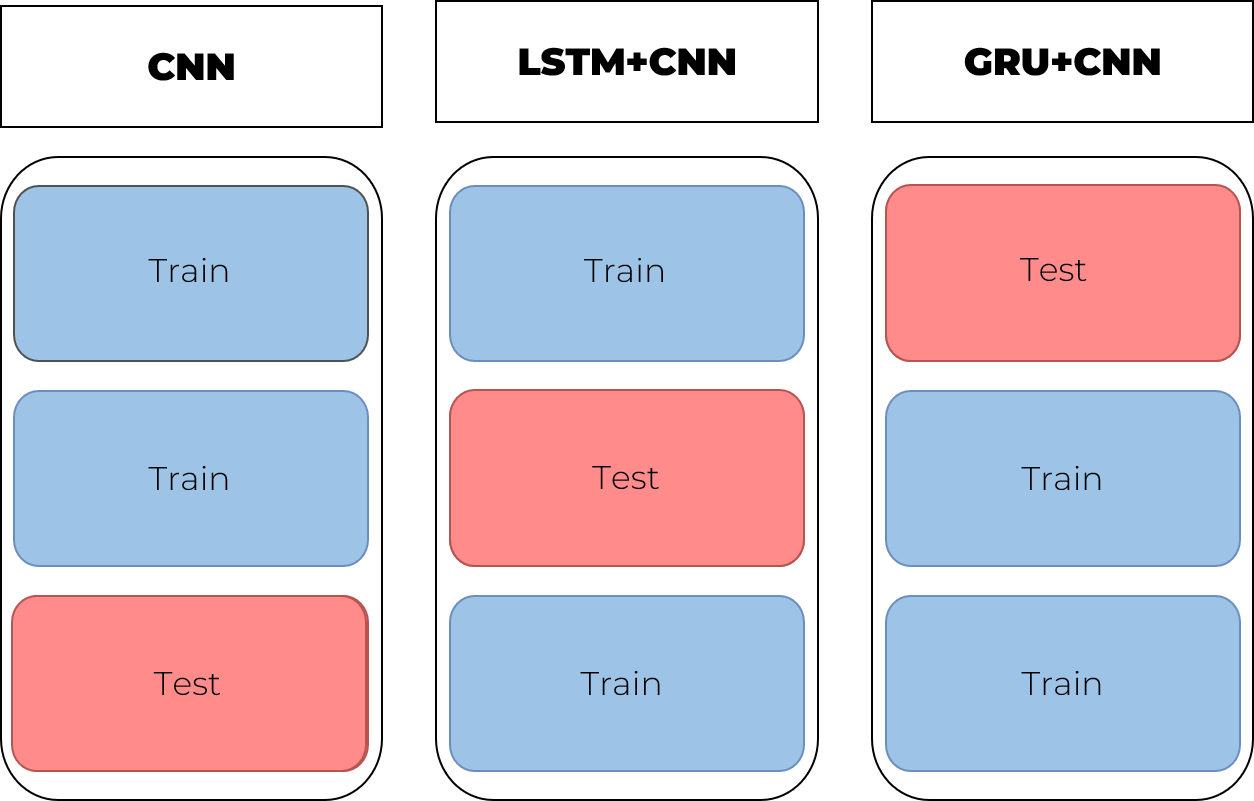
\includegraphics[scale=0.5]{Kfold.png}
    \caption{Stratified K-Foldation для мета моделирования}
    \label{fig:kfold}
\end{figure}
Тренировочный датасет объемом 3.625 миллионов отзывов (результат присоединения датасетов Amazon и IMDB), был разбит на три части, на двух из которых каждая модель обучалась, затем у нее убирался полносвязный слой с sigmoid функцией активации, чтобы получить признаковое описание начальных данных сложной структуры в виде табличной структуры, а на третьей части каждая модель давала предсказания без пересечения между собой. Мета-предсказания, будучи табличными данными, были 
адресованы в классификаторы Random Forest, GBM, SVM, обученные по принципу кросс-валидации (рис. \ref{fig:crossval})
\begin{figure}[H]
    \centering
    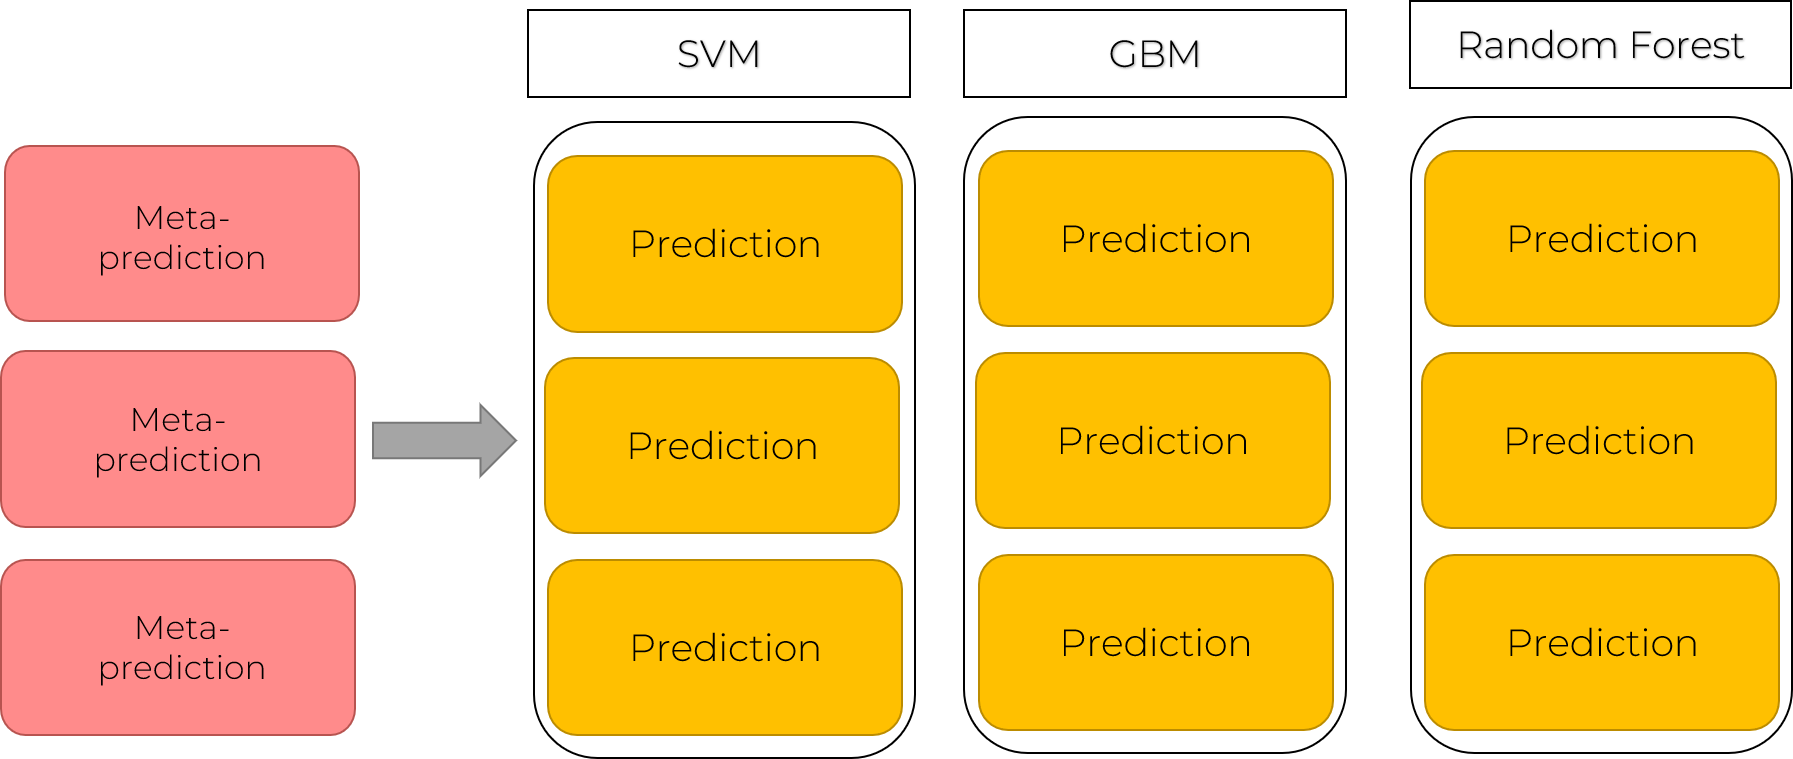
\includegraphics[scale=0.5]{meta.png}
    \caption{Кроссвалидация ансамблированных моделей}
    \label{fig:crossval}
\end{figure}
Усредненный результат трех предсказательных моделей является конечным результатом (рис. \ref{fig:postmeta}):
\begin{figure}[H]
    \centering
    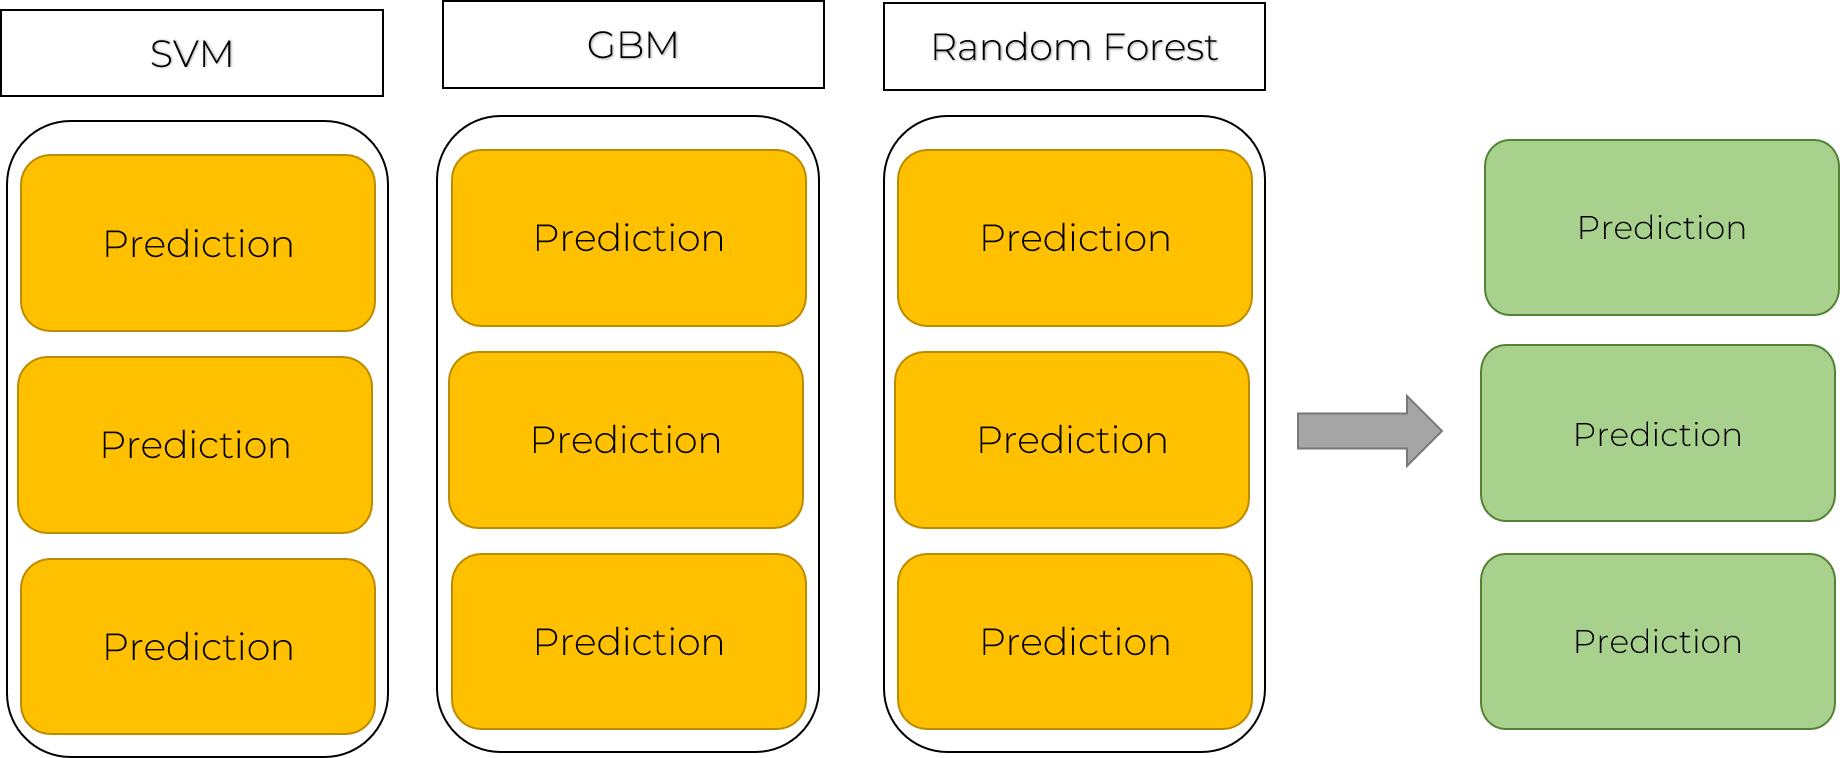
\includegraphics[scale=0.5]{postmeta.png}
    \caption{Ансамблирование и голосование}
    \label{fig:postmeta}
\end{figure}
\subsubsection{Реализация веб-сервиса}
\paragraph{Скраппинг}
\par
Для реализации веб-сервиса по анализу общественного мнения в видеохостинге YouTube были написаны скрапперы с помощью Selenium и Youtube API (так как время работы прототипа с использованием системы автоматизации Selenium было излишне долгим). В рамках Selenium собирается информация о видео (так как это не требует скроллинга) и асинхронно с этим происходит запрос в YouTube API с целью собрать комментарии, количество лайков и ответов на эти комментарии. Затем наскраппленные данные направляются в обученные модели, логиты с последнего слоя которых подаются в классификаторы машинного обучение, затем результат усредняется. Такой же подход был реализован в статье, представляемой в \cite{gagar} с реализацией телеграм-бота. 
\paragraph{Frontend разработка}
В качестве шаблона был использован Bootstrap5 и Jinja2 в качестве шаблонизатора. Верстка шаблонов страниц проделана с помощью HTML и CSS. В рамках работы были произведены масштабирование и адаптация под разные экраны пользователей. Можно говорить о кросс-платформенном использовании web-приложения.
\paragraph{Backend разработка}
В качестве серверной части web-приложения использован фреймворк Flask и локальное хранение данных.
\paragraph{Визуализация}
Главная страница сервиса с навигацией рис. \ref{fig:web1}, \ref{fig:web2}:
\begin{figure}[H]
    \centering
    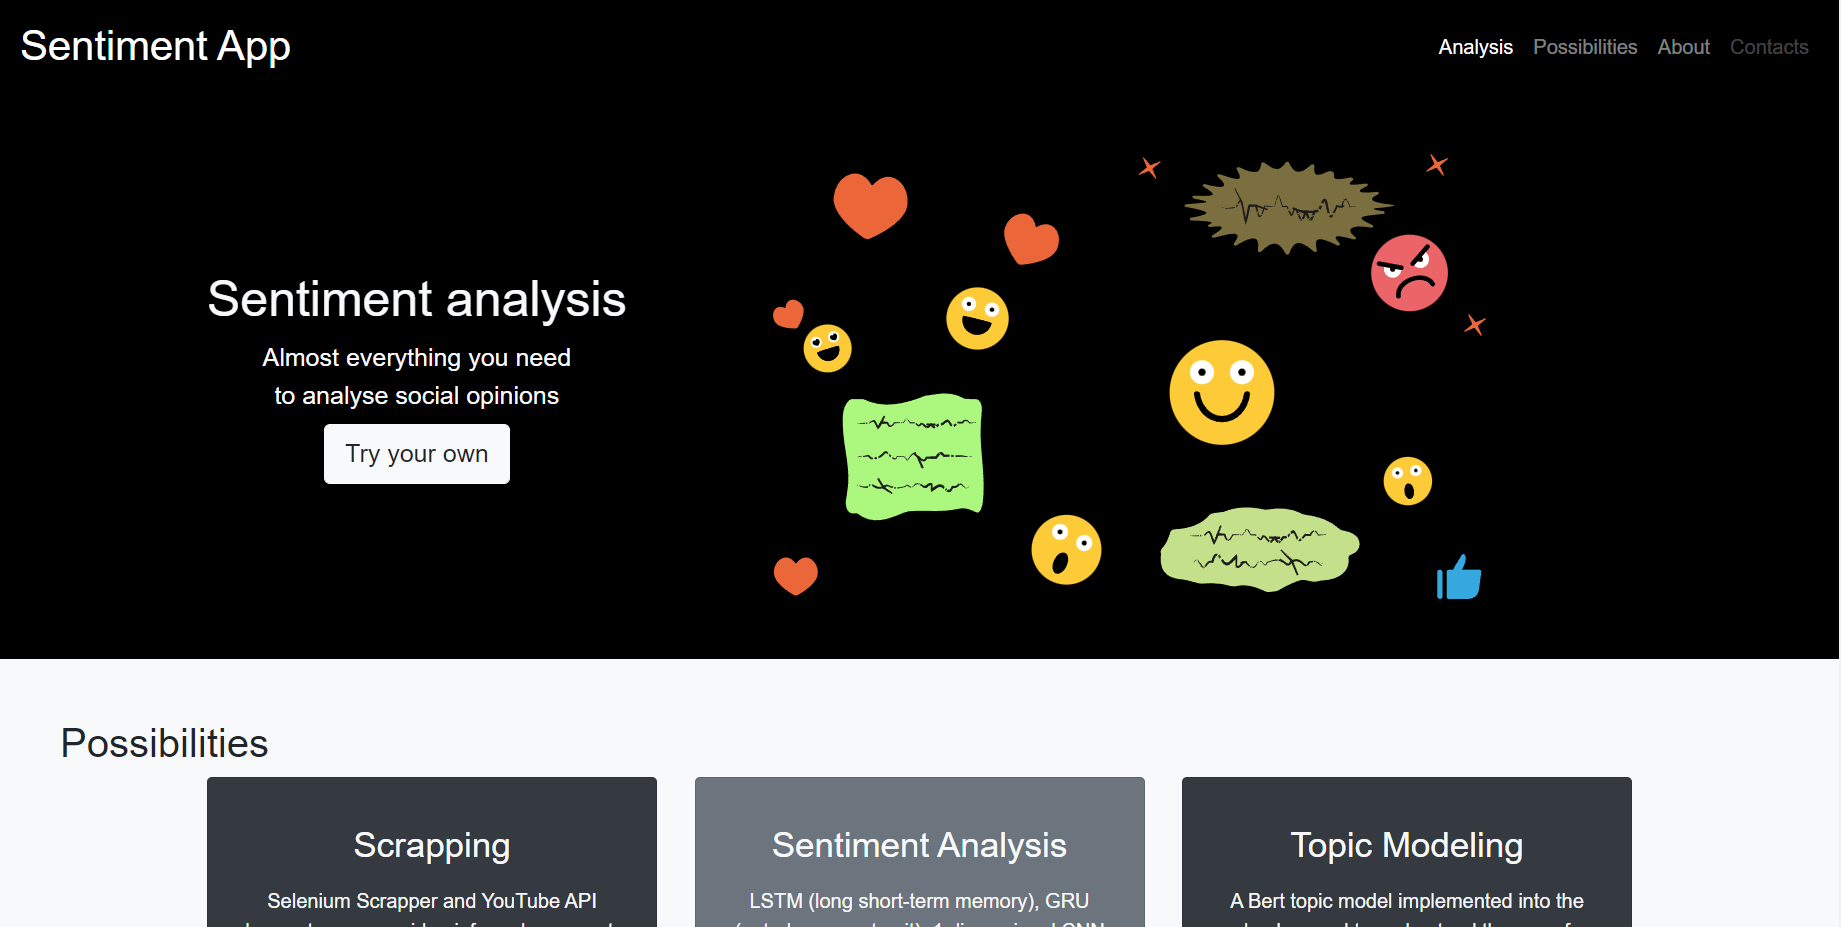
\includegraphics[scale=0.4]{web1.png}
    \caption{Главная страница сервиса}
    \label{fig:web1}
\end{figure}
В поле Link можно вставить ссылку на видео YouTube и запустить таким образом процесс анализа: 
\begin{figure}[H]
    \centering
    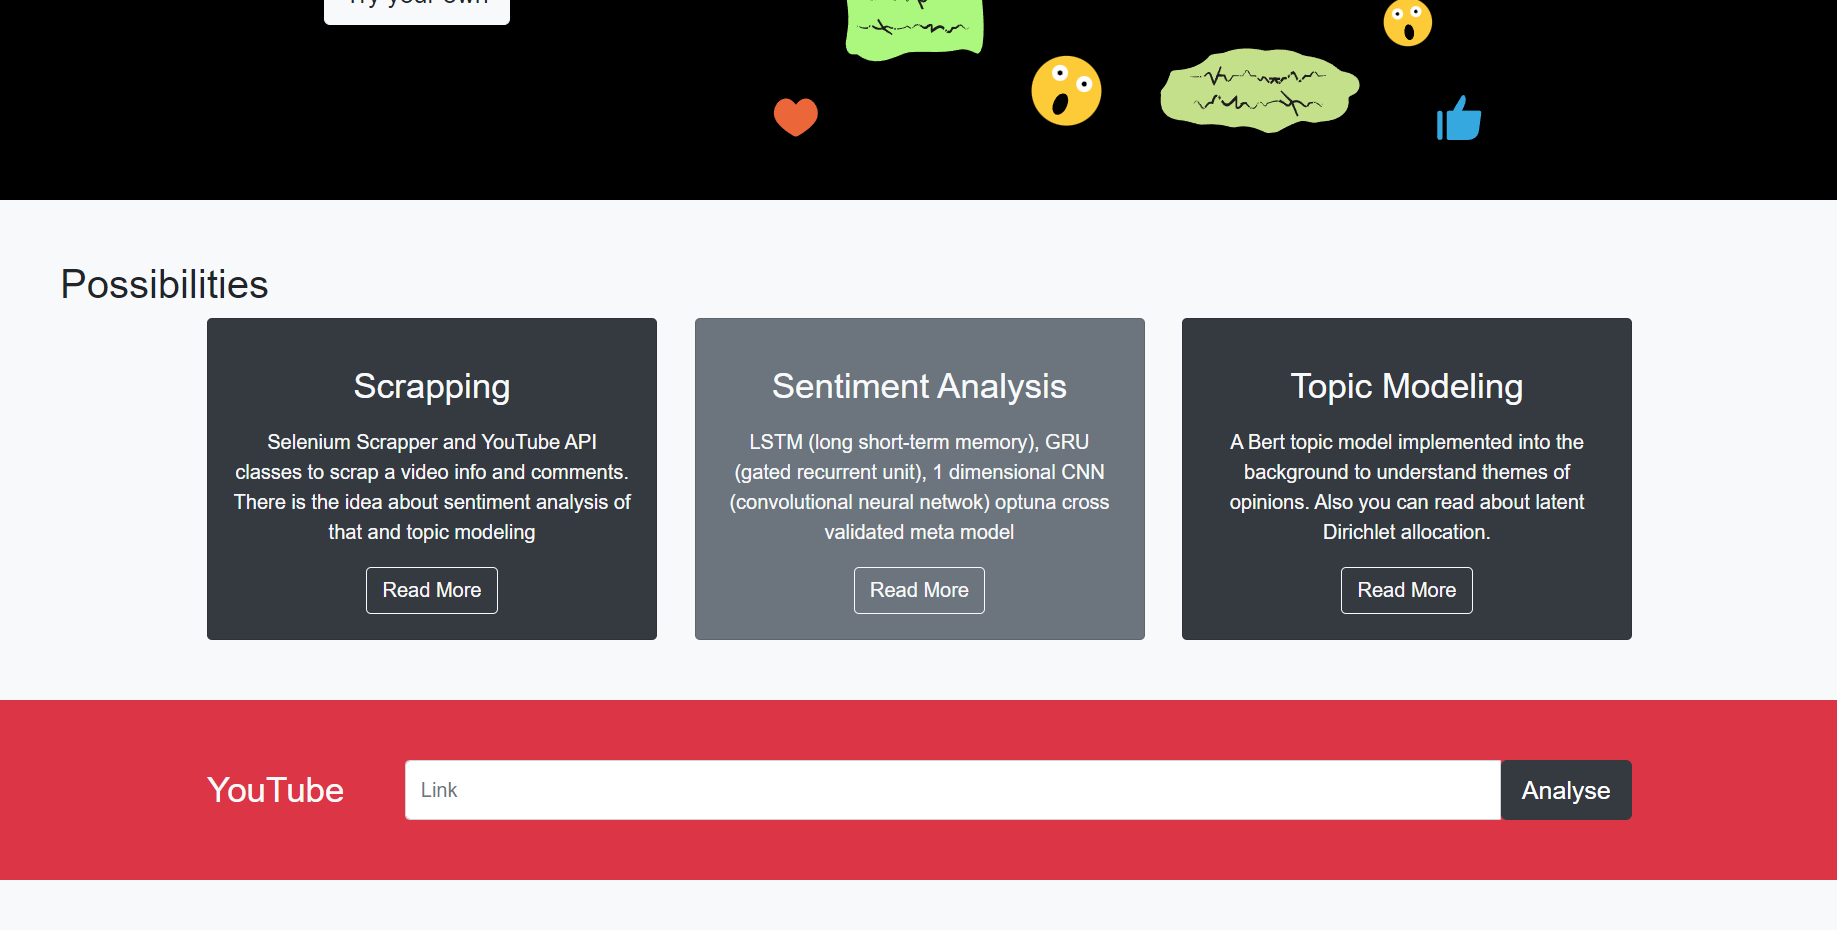
\includegraphics[scale=0.4]{web_mainpage-2.png}
    \caption{Главная страница сервиса}
    \label{fig:web2}
\end{figure}
\begin{figure}[H]
    \centering
    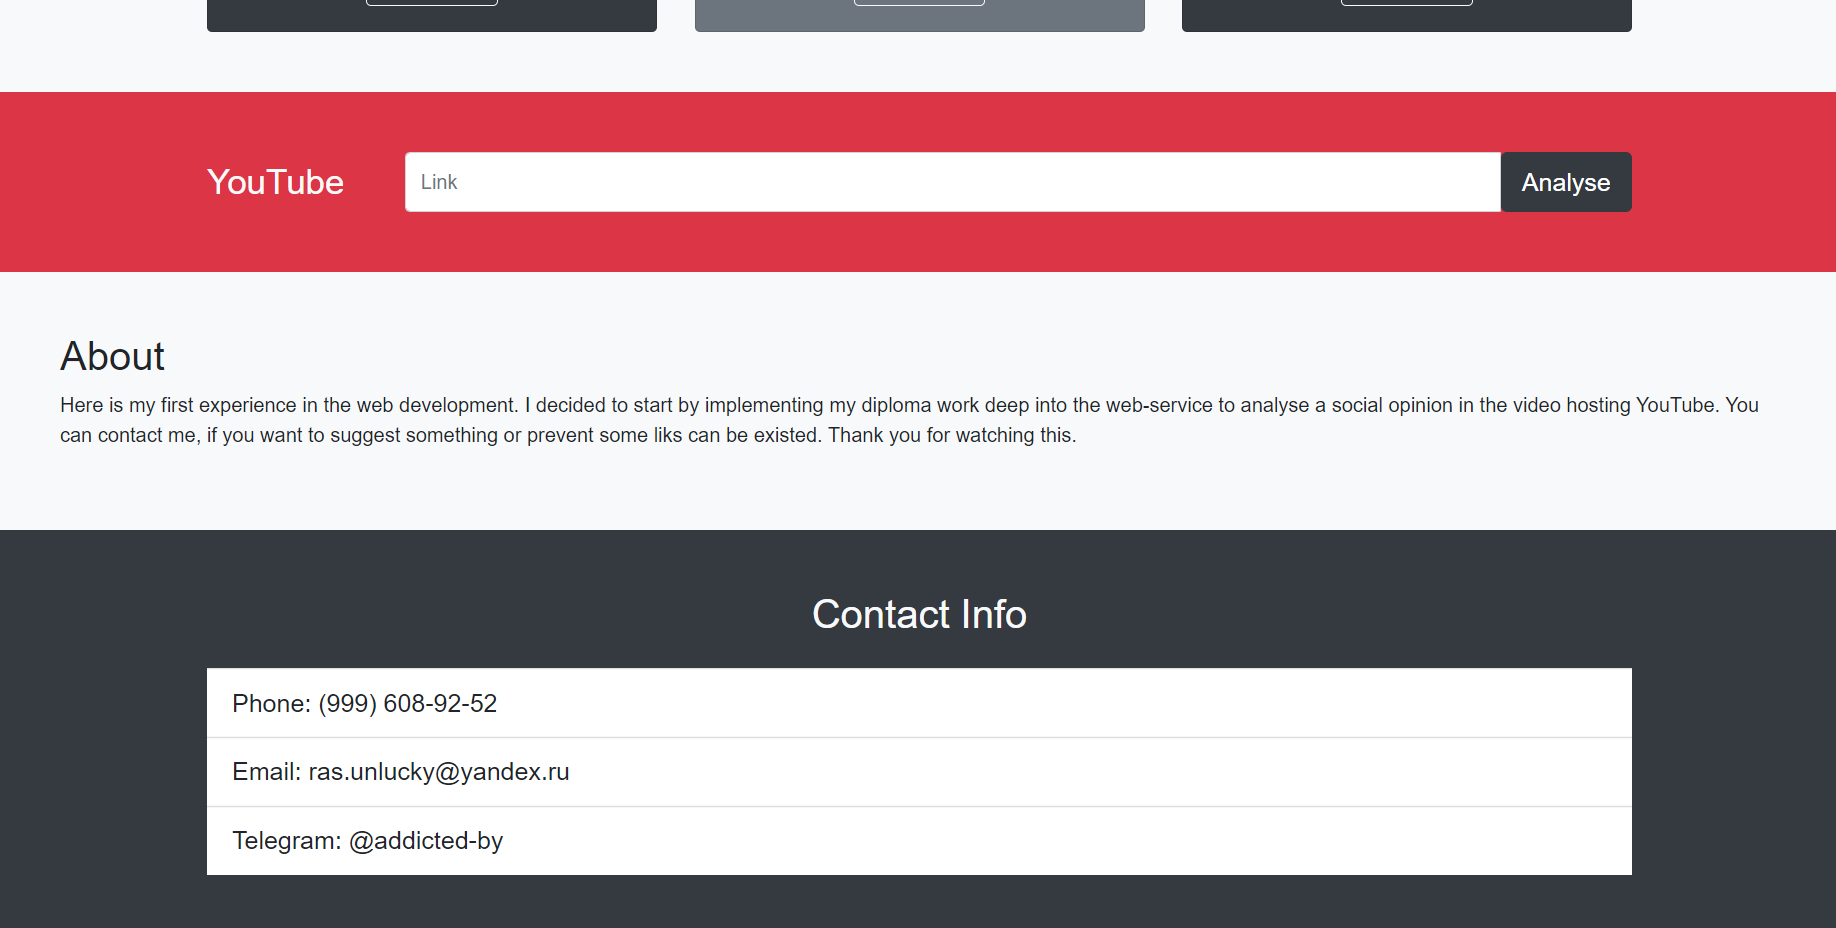
\includegraphics[scale=0.4]{web_mainpage_3.png}
    \caption{Главная страница. Поле ввода}
    \label{fig:web3}
\end{figure}
Как уже было сказано, реализованный сервис является кросплатформенным рис. \ref{fig:mobile}:
\begin{figure}[H]
    \centering
    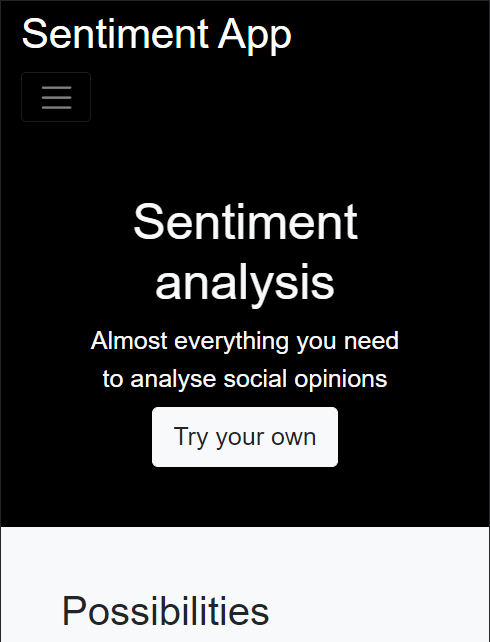
\includegraphics[scale=1.0]{mobile.png}
    \caption{Мобильная версия главной страницы}
    \label{fig:mobile}
\end{figure}
\begin{figure}[H]
    \centering
    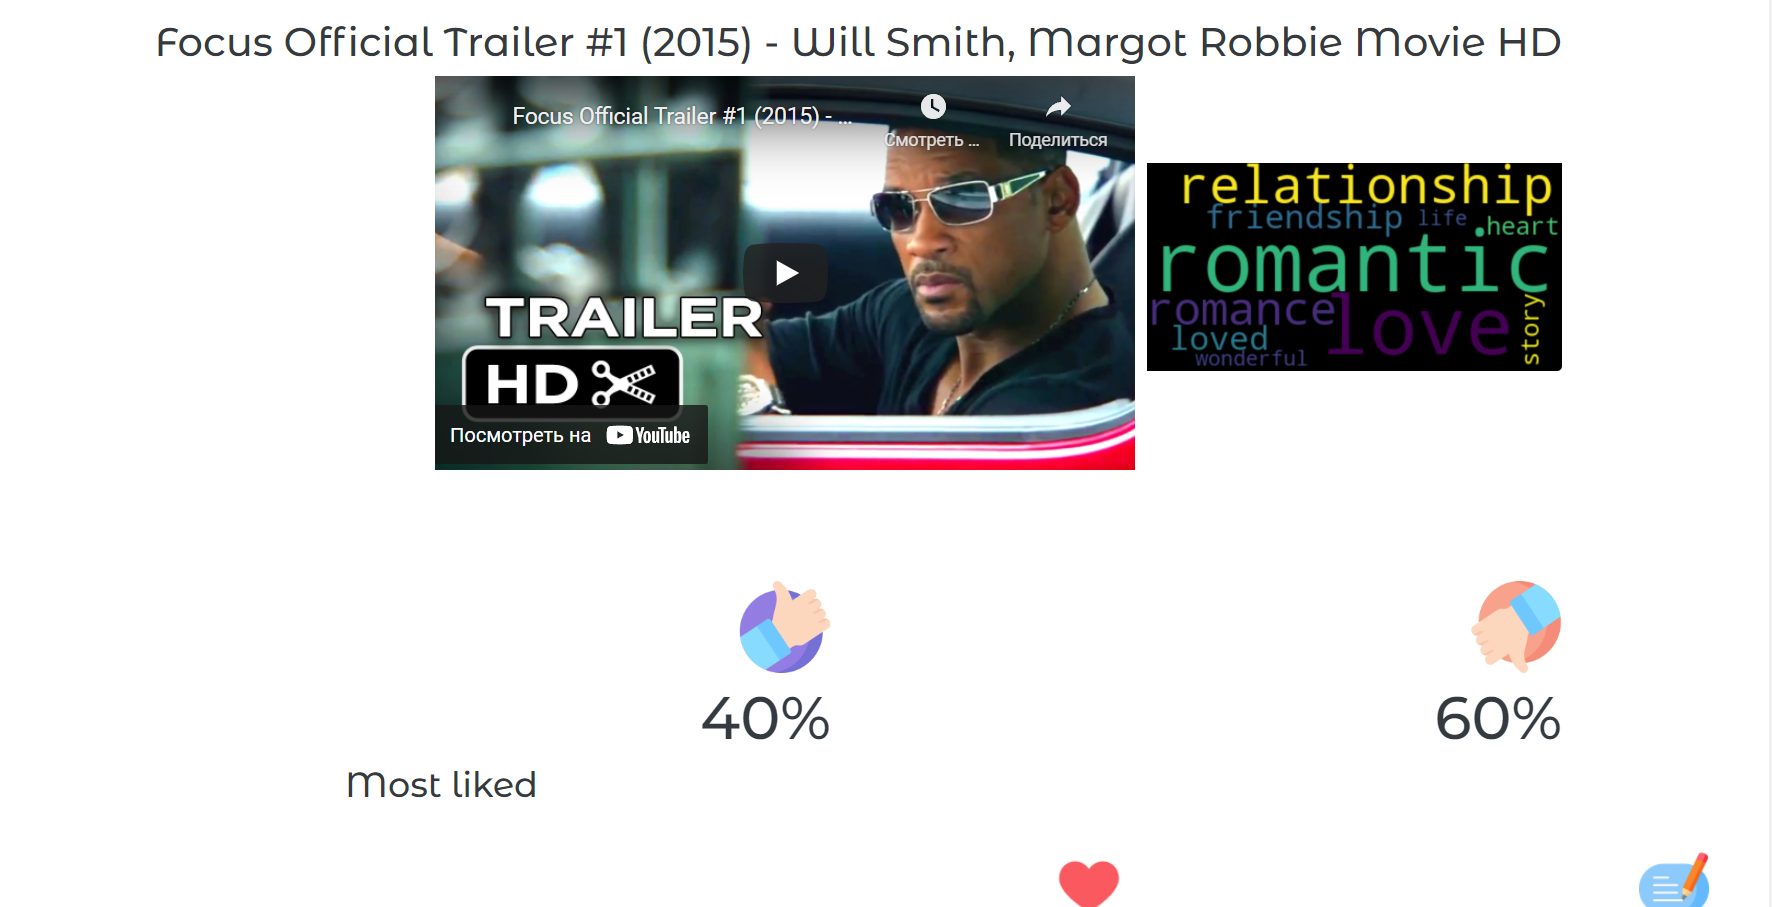
\includegraphics[scale=0.4]{web2.png}
    \caption{Страница анализа}
    \label{fig:web_analysis}
\end{figure}
Кроме того в процессе анализа можно посмотреть на самые интересующие публику (с наибольшим количеством лайков и ответов) комментарии (рис. \ref{fig:web_analysis2}).
\begin{figure}[H]
    \centering
    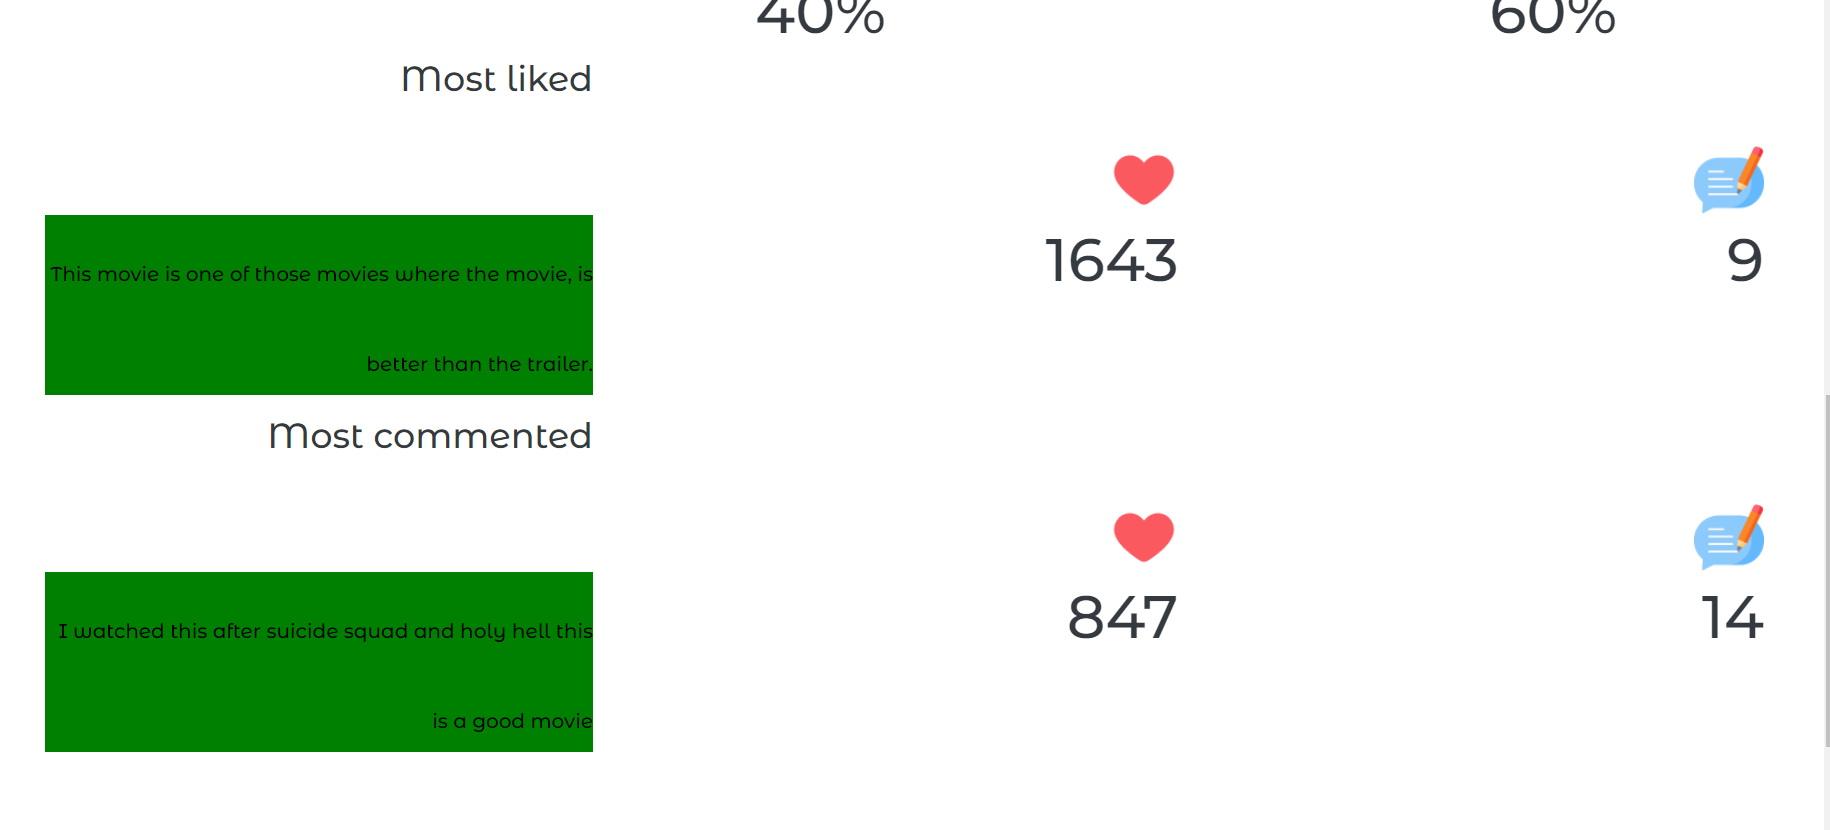
\includegraphics[scale=0.4]{web3.png}
    \caption{Страница анализа -- наиболее популярные комментарии}
    \label{fig:web_analysis2}
\end{figure}

{\CenterChapterHeading\chapter*{ЗАКЛЮЧЕНИЕ}
\newpage
}
\chapter{ЗАКЛЮЧЕНИЕ}

В данной работе были реализованы ансамбль моделей нейросетевого проектирования задачи сентимент-анализа, рассмотрены и использованы модели тематического моделирования (вероятностные и пространственные), а так же показана возможная реализация веб-сервиса, не имеющего аналогов и служащего в качестве завершения дипломной работы. Работа актуальна в силу постоянно растущего объема данных, генерируемых в виде общественных мнений в сети интернет. Задача может быть применена не только к анализу общественных мнений, такой подход применим для рубрикации научных статей, для проведения латентных социальных опросов и как Feature Engineering, например, для задачи предсказания поведения акций на бирже, поскольку общественное мнение и поведение рынка это сильно связанные вещи.

\addtocategory{SourcesGOST}{gagar}
\chapter{СПИСОК ИСПОЛЬЗОВАННЫХ ИСТОЧНИКОВ}
\vspace{-1.0cm}
\begingroup
\let\clearpage\relax
\printbibliography[category=SourcesGOST, title=""]
\vspace{-1.5cm}
\printbibliography[notcategory=SourcesGOST, title=""]
\endgroup
%%%%%%%%%%%%%%%%%%%%%%%%%%%%%%%%%%%%%%%%%%%%%%%%%%%
{\CenterChapterHeading\chapter*{ПРИЛОЖЕНИЯ}
\addcontentsline{toc}{chapter}{ПРИЛОЖЕНИЯ}
\newpage
}
\phantomsection
{\NonNumberedSection\section*{ПРИЛОЖЕНИЕ 1}}
\addcontentsline{toc}{section}{ПРИЛОЖЕНИЕ 1}
\pagestyle{supplement1}

\lstinputlisting[language=python]{./code/models.py}
% \lstinputlisting[language=python]{./code/topic_models.py}
\lstinputlisting[language=python]{./code/scrapping.py}
\lstinputlisting[language=python]{./code/flask.py}


\newpage
\phantomsection
{\NonNumberedSection\section*{ПРИЛОЖЕНИЕ 2}}
\addcontentsline{toc}{section}{ПРИЛОЖЕНИЕ 2}
\pagestyle{supplement2}


\lstinputlisting{./code/source.txt}

%%%%%%%%%%%%%%%%%%%%%%%%%%%%%%%%%%%%%%%%%%%%%%%%%%%
\end{document}
